\documentclass[11pt]{article}
\usepackage[T1]{fontenc}
\usepackage[utf8]{inputenc}
\usepackage{lmodern}
\usepackage[margin=1in]{geometry}
\usepackage{amsmath,amssymb,amsthm,mathtools}
\usepackage{booktabs,longtable,array,enumitem}
\usepackage{microtype}
\usepackage{needspace,etoolbox}
\usepackage{xcolor}
\usepackage{tikz}
\usetikzlibrary{arrows.meta,positioning}
\usepackage{hyperref}
\hypersetup{colorlinks=true,linkcolor=blue!45!black,citecolor=blue!45!black,urlcolor=blue!45!black,pdftitle={A negative solution to the finite lattice representation problem},pdfsubject={A group-theoretic obstruction to finite congruence-lattice representation},pdfauthor={OpenAI}}
\usepackage[nameinlink,capitalize,noabbrev]{cleveref}
\usepackage{url}
\urlstyle{same}
\setlength{\emergencystretch}{2em}
\numberwithin{equation}{section}
\newtheorem{theorem}{Theorem}[section]
\newtheorem{lemma}[theorem]{Lemma}
\newtheorem{proposition}[theorem]{Proposition}
\newtheorem{corollary}[theorem]{Corollary}
\theoremstyle{definition}
\newtheorem{definition}[theorem]{Definition}
\newtheorem{convention}[theorem]{Convention}
\theoremstyle{remark}
\newtheorem{remark}[theorem]{Remark}
\newtheorem{example}[theorem]{Example}
\BeforeBeginEnvironment{theorem}{\Needspace{5\baselineskip}}
\BeforeBeginEnvironment{lemma}{\Needspace{5\baselineskip}}
\BeforeBeginEnvironment{proposition}{\Needspace{5\baselineskip}}
\BeforeBeginEnvironment{corollary}{\Needspace{5\baselineskip}}
\BeforeBeginEnvironment{definition}{\Needspace{5\baselineskip}}
\BeforeBeginEnvironment{convention}{\Needspace{5\baselineskip}}
\BeforeBeginEnvironment{remark}{\Needspace{5\baselineskip}}
\BeforeBeginEnvironment{example}{\Needspace{5\baselineskip}}
\pretocmd{\subsection}{\Needspace{8\baselineskip}}{}{\PackageError{article-layout}{Failed to patch subsection spacing}{}}
\DeclareMathOperator{\Aut}{Aut}
\DeclareMathOperator{\Inn}{Inn}
\DeclareMathOperator{\Out}{Out}
\DeclareMathOperator{\Soc}{soc}
\DeclareMathOperator{\Core}{core}
\DeclareMathOperator{\Rad}{rad}
\DeclareMathOperator{\Con}{Con}
\DeclareMathOperator{\rank}{rank}
\DeclareMathOperator{\GL}{GL}
\DeclareMathOperator{\SL}{SL}
\DeclareMathOperator{\Sp}{Sp}
\DeclareMathOperator{\SO}{SO}
\DeclareMathOperator{\GU}{GU}
\DeclareMathOperator{\SU}{SU}
\DeclareMathOperator{\Hom}{Hom}
\DeclareMathOperator{\End}{End}
\newcommand{\F}{\mathbb F}
\newcommand{\N}{\mathbb N}
\newcommand{\Z}{\mathbb Z}
\newcommand{\Q}{\mathbb Q}
\newcommand{\C}{\mathbb C}
\newcommand{\id}{\operatorname{id}}

\title{A negative solution to the\\finite lattice representation problem}
\author{OpenAI}
\date{September 24, 2026}
\begin{document}
\maketitle
\begin{abstract}
We give a negative solution to the finite lattice representation problem.
We prove that there is a finite nonempty lattice that is not the full
congruence lattice of any finite nonempty algebra of any finite signature.
\end{abstract}
\tableofcontents

\section{Introduction}\label{sec:introduction}

The congruence lattice of an algebra records all of its quotients at once.
The representation theorem of Gr\"atzer and Schmidt says that every
algebraic lattice occurs in this way \cite[Theorem~I, p.~34]{GratzerSchmidt1963}.
The finite version asks for a finite representing algebra whenever the
given lattice is finite. The difference is substantial: a finite
congruence lattice may be represented by an infinite algebra without
providing any finite representation.

Here a finite algebra is a finite nonempty set equipped with finitely many
total operations, each of finite arity. The signature is allowed to
depend on the lattice. Nullary operations and the empty signature are
allowed. We write $\Con(A)$ for the \emph{entire} lattice of congruence
relations on $A$, ordered by inclusion.
Allowing infinitely many finitary operations would give no additional
finite representations. Indeed, a finite carrier has only finitely many
equivalence relations. For each relation that is not a congruence, retain
one operation witnessing its failure of compatibility. The resulting
finite signature has exactly the same congruence lattice.

\begin{theorem}\label{main:congruences}
There exists a finite nonempty lattice $L$ such that
\[
 L\not\cong\Con(A)
\]
for every finite nonempty algebra $A$ of every finite signature.
\end{theorem}

Thus the finite lattice representation problem has a negative answer.
The theorem concerns unrestricted finite universal algebras; it is not
a restriction to a variety, a bound on the carrier size, or an obstruction
to a particular representation method.

P\'alfy and Pudl\'ak proved that the following two universal assertions
are equivalent \cite[Theorem~2]{PalfyPudlak1980}:
every finite lattice is the congruence lattice of a finite algebra, and
every finite lattice is an interval in the subgroup lattice of a finite
group. We establish the failure of the second assertion.

\begin{theorem}\label{main:group}
There exists a finite lattice that is not isomorphic to $[D,G]$ for any
subgroup $D$ of any finite group $G$.
\end{theorem}

Here $[D,G]=\{X:D\le X\le G\}$ carries subgroup inclusion. The equivalence
is global: Theorem~\ref{main:group} implies
Theorem~\ref{main:congruences}, without asserting that a prescribed
individual lattice has the two representation properties simultaneously.
The one-element lattice causes no exception; it is represented by a
one-element algebra and by a trivial subgroup interval.

The constructed subgroup-interval obstruction is self-dual.  It also
cannot be the entire lattice of intermediate fields of a finite separable
extension $E/F$.  Indeed, a
finite normal closure $N/F$ gives an order anti-isomorphism with
\[
 [\operatorname{Gal}(N/E),\operatorname{Gal}(N/F)],
\]
by the Galois correspondence; self-duality would turn such a field
representation into a forbidden subgroup-interval representation.
This is the group--field correspondence discussed in
\cite[Section~3]{PalfyTwisted}.

\subsection{History and the subgroup-interval approach}

The finite problem has several distinct formulations: existence of a
representation, finding a representing algebra, and deciding from a finite
order table whether a representation exists.  McNulty's account separates
these questions and places them in their universal-algebraic setting
\cite[pp.~29--30]{McNulty2015}.  We address the existence question by
ruling out a finite subgroup interval.  The global transfer just stated
is essential: the decorated lattice constructed below is a subgroup-interval
obstruction, and we do not identify it pointwise with the lattice asserted
by Theorem~\ref{main:congruences}.

Two positive representation results clarify the finite requirement.
Pudl\'ak and T\r{u}ma proved that every finite lattice embeds, preserving
meets and joins, into the partition lattice of a finite set
\cite{PudlakTuma1980}.  Such an embedding need not realize the given
lattice as the entire congruence lattice of operations on that set.
On the group side, Repnitski{\u{\i}} and T\r{u}ma represented every finite
lattice as an interval in the subgroup lattice of a countable locally
finite group \cite{RepnitskiiTuma2008}.  Local finiteness still permits
the ambient group to be infinite.

The subgroup-interval approach exposes normal subgroups and primitive
sections to lattice constraints.  Baddeley and Lucchini developed the
reduction of height-two interval questions to finite simple-group problems
\cite{BaddeleyLucchini1997}; Baddeley extended the class of lattice
configurations under consideration \cite{Baddeley1998}.
Further interval reductions were developed by B\"orner and Aschbacher
\cite{Borner1999,Aschbacher2008}.  These results have different hypotheses;
P\'alfy's comparison explains their relationship and the role of almost
simple groups and twisted wreath products \cite[Section~4]{PalfyTwisted}.
In particular, the invariant-subdirect and homomorphism-extension viewpoint
in \cite{PalfyTwisted} is the starting structure for our final reduction.
Aschbacher's minimum-order and signalizer-lattice viewpoint is a related
predecessor of the complementary-socle and extension-kernel arguments.

Lattice shapes can enforce group-theoretic conditions; DeMeo develops
this general perspective and the combination of such requirements
\cite{DeMeoInterval2014}.  Here the particular shapes must do two jobs
simultaneously.  They force uniform restrictions on every possible
simple-group-labelled chain, and they retain the Boolean joins on which
the final extensions must agree.  Uniformity is the obstacle: every
lattice in the construction is finite, but a hypothetical representing
group has no prescribed bound on its order, Lie rank, or field size.

\subsection{The proof in two stages}

Our construction has two stages. The first is a uniform rigidity result
for finite configurations of subgroups. We attach a nonabelian simple
type $T_X$ to selected vertices $X$.  If $D$ is the common bottom,
the unique minimal normal subgroup of $X/\operatorname{core}_X(D)$
is a direct power of $T_X$; here $\operatorname{core}_X(D)$ is the
largest normal subgroup of $X$ contained in $D$.
Special intervals, called fences, test normal subgroups.  Equal labels
give subdirect powers, in which selected simple coordinates are linked
diagonally.  At the comparisons used below, different labels give
coordinate products that can be projected to subgroup intervals of
almost simple groups.
Long chains are supplied with two-edge shortcuts and further interval
tests that make these projections available.  The crucial conclusion
is an \emph{absolute} upper bound
on the length of such a chain when its endpoint labels differ.
The bound must be independent of the finite group in which the
configuration is represented.

The classification of finite simple groups enters this stage through
maximal-subgroup structure and representation theory. A subgroup maximal
in a maximal subgroup of an almost simple group has at most five nonabelian chief
factors \cite[Proposition~8.1]{BurnessLiebeckShalev2017}.
We combine that bound with the fact that coordinate stabilizers in the
common bottom already induce the full local permutation actions on the
simple factors carrying the lower labels.
An elementary bounded-depth action argument then
controls the union of nonabelian simple types in the relevant projected
coordinate stabilizers, rather than just their number at one vertex. Decreasing
bottom cores account for the nonabelian layers lost between socles. These are the
uniformity statements needed before applying finite Ramsey theory.

The remaining classical-group comparisons are controlled by field
parameters, dimension growth, and irreducible restrictions.
The structural starting points are Aschbacher's maximal-subgroup
classification and its classical-group formulations
\cite{Aschbacher1984,KleidmanLiebeck1990}, together with Larsen--Pink's
fixed-type envelope theory \cite{LarsenPink2011}.
Landazuri--Seitz degree bounds separate cross-characteristic growth
\cite{LandazuriSeitz1974,Hasa2014}; Steinberg's representation theory and
L\"ubeck's restricted small-degree classification handle the defining
characteristic \cite{Steinberg1963,SteinbergNotes,Luebeck2001}.
The paper derives the required bounds on whole chains from these inputs;
none of these results alone bounds the lengths of the tested chains.
For defining-characteristic representations, the relevant action on
absolute constituent types is the difference between a source field
shift and an ambient semilinear shift. Their synchronization bounds
composition length independently of the field degree.
After another Ramsey argument, natural modules at later endpoints
restrict irreducibly to earlier ones.  The irreducible-triple input
comes from Seitz's classification and the corrections of Cavallin and
Testerman, in the formulation of Burness and Testerman
\cite{Seitz1987,CavallinTesterman2019,BurnessTesterman2018}.
We use it twice: first with a bound on the composition length of the
ambient natural module on the smallest subgroup
(Lemma~\ref{irr:rank-length}), and then with an intervening simple
subgroup of strictly larger rank whose natural module is irreducible
on that smallest subgroup (Lemma~\ref{irr:intervening}).
These hypotheses control the twisted-diagonal spin families.
The resulting rank bounds are incompatible with a sufficiently long
chain and its two-edge shortcuts.

In the second stage, we build one finite lattice from a Boolean lattice
of rank four and a small additional configuration, called the detector.
The chain tests are inserted in both required orders while preserving
the original Boolean meets and joins.  Their length is chosen from the
absolute bound, before any representing group is considered.

Suppose the resulting lattice is represented by $[D,G]$, with $|G|$
minimal among representations in either orientation.  The global fence
gives a socle $S\cong T^I$ and $G=DS$; minimality gives $D\cap S=1$.
Equality of the forward labels forces every proper nonzero original
Boolean vertex $Y$ to meet $S$ in a subdirect subgroup, meaning one
which projects onto every simple coordinate.  Fixing a coordinate
gives its stabilizer $A\le D$ and an action
\[
                   \alpha:A\longrightarrow\Aut(T).
\]
A $D$-invariant subdirect subgroup corresponds to a subgroup $U$ with
$A\le U\le D$ and a homomorphism $\beta:U\to\Aut(T)$ extending
$\alpha$.  This correspondence reverses inclusion.  It realizes the
reversed upper filter above $Y$ as the actual group interval $[A,U_Y]$.

The reverse chain tests make the socles of
$U_Y/\operatorname{core}_{U_Y}(A)$ powers of one simple group $R$,
which need not equal $T$.
The detector ensures $\alpha(A)\ge\Inn(T)$.  Read the original
Boolean copy in reverse order.  Proper Boolean unions give extensions
on generated domains that agree on their overlaps.  For a full union,
the corresponding forward vertices meet at $D$, so their intersections
with $S$ have trivial intersection.  A common extension would produce
a nontrivial subdirect subgroup in this intersection and is therefore
forbidden.

The final argument forces that forbidden extension.  If the core of
$A$ in an atom domain had trivial image, compatible lifts of socle
factors on the three rank-two faces through that atom would already
produce a common extension.  Hence every atom core has image containing
$\Inn(T)$.  Intersections give the same
property for larger proper faces.  A least normal subgroup of $A$
with this inner image is then normal in all the relevant domains;
conjugation on its quotient isomorphic to $T$ supplies their common
extension.  This is the contradiction.

\subsection{Structure and scope of the proof}

Section~\ref{sec:framework} develops the lattice tests and factor
transport. The central group-theoretic result is
Theorem~\ref{cls:chain-rigidity}, stated in
Section~\ref{sec:classification} and proved in
Sections~\ref{sec:classification}--\ref{sec:rigidity}.
These sections control, successively, factor actions and simple types,
field and dimension growth, algebraic lifts along paths,
natural-module composition length, and irreducible restrictions.
Section~\ref{sec:lattices} constructs a finite lattice realizing all
the tests. Sections~\ref{ext:section} and~\ref{glue:section} reduce a
hypothetical representation to an extension configuration and rule
it out by Boolean gluing, proving Theorem~\ref{main:group}.

The finite lattice is specified by finitely many private-branch
insertions with a sufficiently large finite chain parameter.
An explicit numerical value of that parameter is unnecessary for the
existence conclusion. Its existence follows from bounds that are
uniform over all possible finite-group representations.

All groups are finite unless called algebraic groups. Algebraic
groups occur only in the representation-theoretic part of the proof
and are taken over algebraically closed fields of positive
characteristic, with central covers and the stated special isogenies
when needed. We use the classification of finite simple groups and
identify each additional classification or representation input at
its point of application. The new uniformity, lifting, lattice
bookkeeping and gluing deductions are proved explicitly.

\section{Fences, socles, and coordinate transport}
\label{sec:framework}

All groups in this section are finite. A vertex of a subgroup interval is
written as a capital letter and identified with the corresponding subgroup.
The common bottom is denoted by $D$. We first record the normal-subgroup
test that will give the vertices their simple-group labels. We then explain
the two different kinds of factor transport: diagonal merging when the
simple type is unchanged, and coordinate products when it changes.

\subsection{The normal-subgroup test}

\begin{definition}
A bounded lattice interval $[a,b]$ is \emph{fenced} if it has an interior
element and, for each $a<c<b$, there are $a<u<v<b$ such that
\[
 c\wedge u=c\wedge v=a,
 \qquad c\vee u=c\vee v=b.
\]
Thus the two comparable elements $u,v$ are both complements of $c$ in
the interval. The requirement of an interior element excludes vacuous
fences on covering intervals. Length always counts edges.
\end{definition}

\begin{lemma}[Normal-subgroup test]
\label{frm:normal-test}
Suppose that $[D,X]$ is fenced. If $R\trianglelefteq X$, then either
$R\le D$ or $DR=X$. In particular, $[D,X]$ is not modular.
The same assertion applies to a normal subgroup of $X/F$ whenever
$F\trianglelefteq X$ and $F\le D$, with bottom $D/F$.
\end{lemma}

\begin{proof}
For $D\le U\le V\le X$, the normality of $R$ and the subgroup
modular identity give
\begin{equation}
 \label{frm:normal-modular-identity}
 (DR\vee U)\wedge V
   =(RU)\cap V
   =U(R\cap V)
   =U\vee(DR\wedge V).
\end{equation}
If $D<DR<X$, apply the fence to $DR$ and its comparable complements
$U<V$. Equation~\eqref{frm:normal-modular-identity} would give $V=U$.
Thus $DR$ is an endpoint. In a modular lattice the same identity holds
with any element in place of $DR$, so the existence of a fence also
excludes modularity. Finally, taking inverse images identifies
$[D/F,X/F]$ with $[D,X]$.
\end{proof}

We will repeatedly use the following explicit form of the subgroup
correspondence. If $R\trianglelefteq X$ and $X=DR$, then
\begin{equation}
 \label{frm:supplement-correspondence}
 [D,X]\longrightarrow
 \{E\le R:D\cap R\le E,\ E\text{ is normalized by }D\},
 \qquad U\longmapsto U\cap R
\end{equation}
is an order isomorphism, with inverse $E\mapsto DE$. Indeed
$U=D(U\cap R)$ for $D\le U\le DR$, and $(DE)\cap R=E$ when
$D\cap R\le E$. This correspondence includes every overgroup of $D$.

\begin{lemma}[Labels]
\label{frm:labels}
Suppose that $[D,X]$ is fenced, and put
\[
 F_X=\operatorname{core}_X(D)
     =\bigcap_{g\in X}D^g.
\]
Then $X/F_X$ has a unique minimal normal subgroup
\begin{equation}
 \label{frm:socle-label}
 S_X=N_X/F_X\cong T_X^{m_X},
\end{equation}
where $T_X$ is nonabelian simple and $N_X$ is its full inverse image in
$X$. Moreover,
\[
 X=DN_X.
\]
Every nontrivial normal subgroup of $X/F_X$ contains $S_X$, and
\[
 C_{X/F_X}(S_X)=1.
\]
In particular, $X/F_X$ has no nontrivial soluble normal subgroup.
If $I_X$ is the set of simple direct factors of $S_X$, then $D$ and $X$
induce the same transitive permutation group on $I_X$.
\end{lemma}

\begin{proof}
Factor out $F_X$, so that the action of $X$ on the cosets of $D$ is
faithful. Lemma~\ref{frm:normal-test} says that every nontrivial normal
subgroup supplements $D$, or equivalently is transitive in this action.
Let $M$ be a minimal normal subgroup. If $M$ were abelian,
\eqref{frm:supplement-correspondence} would identify $[D,X]$ with an
interval of $D$-invariant subgroups of an abelian group. The latter lattice
is modular: intersection is its meet and subgroup product is its join.
This contradicts Lemma~\ref{frm:normal-test}.

If $M'$ were another minimal normal subgroup, then
$[M,M']\le M\cap M'=1$. Every $D$-invariant subgroup of $M$ would
therefore be normalized by $DM'=X$, and so would be either $1$ or $M$.
The correspondence~\eqref{frm:supplement-correspondence} would leave
at most two elements in $[D,X]$, again a contradiction.

A finite minimal normal subgroup is characteristically simple, hence
a direct product of isomorphic simple groups. Since $M$ is nonabelian,
these simple groups are nonabelian. Conjugation by $X$ is transitive on
the direct factors: otherwise the product of one orbit of factors would
be a proper nontrivial normal subgroup of $X$ contained in $M$. This
proves~\eqref{frm:socle-label}. Every nontrivial normal subgroup contains
a minimal normal subgroup and therefore contains $M$. Its centralizer
is normal and intersects $M$ in $Z(M)=1$, so that centralizer is trivial.
The assertion about soluble normal subgroups follows as well.

Finally $X=DM$. Inner automorphisms of $M$ fix each of its simple direct
factors. Thus $D$ and $X$ have the same image on their factor set.
Restoring $F_X$ proves the statements as written.
\end{proof}

We call an $X$ satisfying Lemma~\ref{frm:labels} a \emph{labelled
vertex}, and call the isomorphism type of $T_X$ its \emph{simple type}.
The preceding argument is also the strongly nonmodular normal-subgroup
argument in \cite[Lemma~3.6]{PalfyTwisted}.

\begin{corollary}[Bottlenecks]
\label{frm:bottleneck}
Let $D<B\le Z$, suppose that $[D,B]$ is fenced, and suppose that $B$
is comparable with every member of $[D,Z]$. If $R\trianglelefteq Z$
and $R\nleq D$, then
\[
 B=D(R\cap B).
\]
Consequently a soluble normal subgroup of $Z$ is contained in $D$.
If $R,Q\trianglelefteq Z$ and
\[
 [R,Q]\le F\trianglelefteq Z,\qquad F\le D,
\]
then at least one of $R,Q$ is contained in $D$.
These conclusions also hold with $B=Z$.
\end{corollary}

\begin{proof}
The subgroup $R\cap B$ is normal in $B$. Suppose first that
$R\cap B\le D$. If $B\le DR$, then
\[
 B=B\cap DR=D(B\cap R)=D,
\]
a contradiction. Comparability therefore gives $DR\le B$, whence
$R=R\cap B\le D$. Its contrapositive, followed by
Lemma~\ref{frm:normal-test} in $B$, gives the asserted supplementation.
The image of $R\cap B$ modulo $F_B$ then contains the nonabelian
socle $S_B$, by Lemma~\ref{frm:labels}. This is impossible if $R$ is
soluble. For the final assertion, $F\le F_B$ because $F$ is normal in
$B$ and contained in $D$. If both $R$ and $Q$ escaped $D$, their
intersections with $B$ would both map over $S_B$, while their images
would commute. This would make $S_B$ abelian.
\end{proof}

\subsection{Subdirect powers and unchanged simple types}

For a direct product $T^I=\prod_{i\in I}T_i$, with each $T_i\cong T$,
a subgroup is \emph{subdirect} if all coordinate projections are
surjective. A \emph{full diagonal strip} on a nonempty subset $J\subseteq I$
is a subgroup obtained by identifying all the $T_j$, $j\in J$, by
isomorphisms, and putting identity elements outside $J$.
We recall the standard diagonal-strip description
\cite[Lemma~2.1]{PalfyTwisted}, including its behavior under inclusion.

\begin{lemma}[Subdirect powers]
\label{frm:subdirect}
Let $T$ be nonabelian simple. Every subdirect subgroup $E\le T^I$
is a direct product of full diagonal strips on the parts of a partition
of $I$. Both the partition and the coordinate identifications within
each part are determined by $E$. An inclusion of subdirect subgroups
corresponds to a refinement of these parts, with the existing
identifications restricted to the smaller parts.
\end{lemma}

\begin{proof}
Induct on $|I|$, separating the last coordinate. The projection to the
other coordinates is, by induction, a product $T^r$ of diagonal strips.
We have a subdirect subgroup of $T^r\times T$. The kernels of its two
projections are normal in the respective factors. The kernel on the last
$T$ is either $T$, in which case this is the full product, or $1$, in
which case the subgroup identifies a quotient of $T^r$ with $T$.
Normal subgroups of $T^r$ are products of its simple direct factors, so
that quotient is one of the factors. The last coordinate is therefore
joined to exactly one existing strip.

Two coordinates belong to the same strip precisely when the projection
of $E$ to their product is the graph of an isomorphism rather than the
full product. This characterizes the partition and its links, and also
proves the assertion about inclusion.
\end{proof}

\begin{proposition}[Equal-type transport]
\label{frm:equal-transport}
Let $D<X<Y$ be labelled vertices. Then $F_Y\le F_X$, and $T_X$ is
isomorphic to a section of $T_Y$. Put
\[
 E_X=(X\cap N_Y)/F_Y\le S_Y.
\]
The following conditions are equivalent:
\begin{enumerate}[label=\textup{(\roman*)}]
 \item $T_X\cong T_Y$;
 \item $E_X$ is subdirect in $S_Y$.
\end{enumerate}
When they hold, the quotient map induces an isomorphism
\begin{equation}
 \label{frm:equal-socle-identification}
 E_X\xrightarrow{\ \sim\ }S_X,
 \qquad
 N_X=F_X(X\cap N_Y),
 \qquad F_X\cap N_Y=F_Y.
\end{equation}
Moreover $m_X<m_Y$, and the strip supports give a canonical
$X$-equivariant surjection
\begin{equation}
 \label{frm:equal-support-map}
 \sigma_{YX}:I_Y\longrightarrow I_X.
\end{equation}
For three comparable labelled vertices of the same simple type these
maps compose:
$\sigma_{ZX}=\sigma_{YX}\sigma_{ZY}$.
\end{proposition}

\begin{proof}
The normal subgroup $F_Y$ of $X$ is contained in $D$, so $F_Y\le F_X$.
Since $Y=DN_Y$ and $D\le X$,
\[
 X=D(X\cap N_Y).
\]
The image of $E_X$ in $X/F_X$ is a nontrivial normal subgroup and
therefore contains $S_X$. Every simple composition factor of a subgroup
of a direct product is a section of one of the factors: projection to
one coordinate gives an exact sequence whose kernel lies in the product
of the remaining coordinates, and induction applies. Thus $T_X$ is a
section of $T_Y$.

If $T_X\cong T_Y$, some coordinate projection of $E_X$ is all of $T_Y$;
otherwise none of those smaller groups could have a composition factor
of order $|T_Y|$. The transitive action of $D$ on $I_Y$ makes all the
projections surjective. Conversely, suppose $E_X$ is subdirect.
Lemma~\ref{frm:subdirect} expresses it as a product of diagonal copies
of $T_Y$. The action of $D$ on those copies is transitive. Since
$X/F_Y=(D/F_Y)E_X$, the subgroup $E_X$ is minimal normal in $X/F_Y$.
Its intersection with $F_X/F_Y$ is either trivial or all of $E_X$.
The latter would imply $X=D$, which is excluded. Its image is therefore
the unique minimal normal subgroup $S_X$, proving the equivalence and
\eqref{frm:equal-socle-identification}.

There are $m_X$ strips on $m_Y$ coordinates. If $m_X=m_Y$, every strip
is a singleton, so $E_X=S_Y$ and $X=Y$. Thus $m_X<m_Y$.
The quotient identification with $S_X$ assigns to every strip its
actual simple factor in $I_X$ and defines~\eqref{frm:equal-support-map}.
The subgroup $E_X$ is normal in $X/F_Y$, and its quotient identification
with $S_X$ commutes with conjugation by $X$; hence this support map is
$X$-equivariant.

For composition, factor out $F_Z$ and let $E_Y=Y\cap N_Z$.
We have $N_Y=F_YE_Y$ and $F_Y\cap E_Y=1$. Since $F_Y\le X$,
\[
 X\cap N_Y=F_Y(X\cap E_Y)=F_Y(X\cap N_Z).
\]
Thus the subdirect subgroup used for $X<Y$ is the image of the one
used for $X<Z$ under the already specified identification
$E_Y\cong S_Y$. Refinement of its strip partition is exactly
composition of the support maps.
\end{proof}

In particular, a change of simple type is strict in order:
$T_X\not\cong T_Y$ implies $|T_X|<|T_Y|$. A section of a finite group
having its full order must be the group itself.

\subsection{Products and one-coordinate intervals}

Fix a labelled upper vertex $Y$. Work modulo $F_Y$ when discussing its
socle $S_Y=T^{I_Y}$. Conjugation by $D$ is transitive on $I_Y$.
Choose a reference coordinate and transport identifications of the other
coordinates by elements of $D$. Notation such as $P^{I_Y}$ always means
the product of these transported copies. The subgroup in the reference
coordinate must be invariant under the corresponding factor stabilizer;
this is precisely the condition that makes the transported product
invariant under the whole group in question.

Call $D\le Z\le Y$ \emph{saturated relative to $Y$} if
$(Z\cap N_Y)/F_Y$ is the product of its coordinate projections.
The proof below uses the product--subdirect intersection arguments of
\cite[Lemmas~2.12 and~2.13]{PalfyTwisted} to obtain the required saturation.

\begin{proposition}[Strict products and saturation]
\label{frm:strict-product}
Let $D\le X<Y$, where $Y$ is labelled. Suppose that the coordinate
projections of
\[
 B=(X\cap N_Y)/F_Y
\]
are proper and nontrivial. If $[X,Y]$ is fenced, or if $X$ is a coatom
of $[D,Y]$, then $X$ is saturated relative to $Y$.

Once $B=P^{I_Y}$ is such a product, no proper subdirect subgroup of
$S_Y$ contains $B$. Every coatom of $[X,Y]$, and every intersection
of these coatoms, is saturated relative to $Y$.
These assertions do not require $X$ to be labelled. For labelled
$X<Y$ of different simple types the projection hypothesis holds.
\end{proposition}

\begin{proof}
Factor out $F_Y$, and let $C$ be the product of the coordinate
projections of $B$. It is $X$-invariant. The correspondence
\eqref{frm:supplement-correspondence}, with bottom $X$ and normal
subgroup $S_Y$, identifies $[X,Y]$ with the $X$-invariant subgroups of
$S_Y$ containing $B$.

Suppose $B<C<S_Y$. If $U<V$ are comparable complements of $XC$,
put $E_U=U\cap S_Y$ and $E_V=V\cap S_Y$. Their projections already
contain the projections of $C$. Hence projecting
$\langle E_U,C\rangle=S_Y$ shows that $E_U$ is subdirect; the same
holds for $E_V$.

Every link within a strip of $E_U$ carries the projection of $B$ in one
coordinate onto its projection in the other, because $B\le E_U$.
Consequently $E_U\cap C$ is a product of independent diagonal copies
of those nontrivial projections, one for each strip of $E_U$.
The proper inclusion $E_U<E_V$ splits at least one strip, by
Lemma~\ref{frm:subdirect}. Intersecting with $C$ then permits an
additional independent nonidentity coordinate value, and gives
$E_U\cap C<E_V\cap C$. This contradicts the required equality of
both intersections with $B$. A fence therefore forces $B=C$.
If $X$ is a coatom, $B<C<S_Y$ directly contradicts maximality.

A proper subdirect subgroup has a link between two distinct coordinates.
The full product $P^{I_Y}$ contains an element which is identity in the
first of these coordinates and nonidentity in the second, contradicting
that link. Now let $Z$ be a coatom above $X$. If its projections were
full, it would be such a proper subdirect subgroup. Otherwise its product
closure is proper, and maximality forces it to equal that closure.
Intersections of products are products.

Finally, for different labelled simple types, the projections are
nontrivial because their image contains $S_X$, and transitivity makes
all of them nontrivial. If one were full, all would be full, contradicting
Proposition~\ref{frm:equal-transport}.
\end{proof}

\begin{proposition}[One-coordinate projection]
\label{frm:projection}
Let $D\le X<Y$, with $Y$ labelled, and suppose that
\[
 (X\cap N_Y)/F_Y=P_X^{I_Y},\qquad 1<P_X<T_Y.
\]
Suppose also that $X$ is an intersection of coatoms of $[X,Y]$;
a coatom itself is allowed. Fix $i\in I_Y$ and let
\[
 \rho:Y_i\longrightarrow\operatorname{Aut}(T_Y)
\]
be the action of its factor stabilizer on that coordinate. Identify
$T_Y$ with its inner automorphism group, and put
$H_* = \rho(X_i)$. Then
\begin{equation}
 \label{frm:inner-bottom}
 H_*\cap T_Y=P_X.
\end{equation}
The saturated overgroups of $X$ form a sublattice of $[X,Y]$, and
\begin{equation}
 \label{frm:coordinate-interval}
 Z\longmapsto K_Z=\rho(Z_i)=H_*P_Z,
 \qquad (Z\cap N_Y)/F_Y=P_Z^{I_Y},
\end{equation}
is an isomorphism from that sublattice onto the entire ordinary subgroup
interval $[H_*,H_*T_Y]$. Original covering relations between saturated
vertices remain covering relations after projection. In particular, a
strict change of simple type at a cover yields a maximal subgroup of an
almost simple group, supplementing its simple socle.
\end{proposition}

\begin{proof}
For a coatom $M$ above $X$, Proposition~\ref{frm:strict-product} writes
its intersection with $S_Y$ as $P_M^{I_Y}$, with $1<P_M<T_Y$.
Let $J=H_*\cap T_Y$. It normalizes $P_M$, so
\[
 P_MJ\le N_{T_Y}(P_M)<T_Y.
\]
The last inequality follows from simplicity and $1<P_M<T_Y$.
Both $P_M$ and $J$ are $H_*$-invariant, and their product therefore
transports to a saturated overgroup of $M$ which is still proper in $Y$.
Maximality gives $J\le P_M$. Intersecting over the coatom representation
of $X$ gives $J\le P_X$; the reverse inclusion is immediate. This proves
\eqref{frm:inner-bottom}.

Products above $P_X^{I_Y}$ correspond precisely to $H_*$-invariant
subgroups $P_Z\le T_Y$ containing $P_X$. By
\eqref{frm:inner-bottom}, these in turn correspond precisely to the
subgroups $K_Z$ of $H_*T_Y$ containing $H_*$: the two maps are
$P_Z\mapsto H_*P_Z$ and $K_Z\mapsto K_Z\cap T_Y$.
Since $Z=X P_Z^{I_Y}$ and the product fixes the coordinate set,
$Z_i=X_iP_Z^{I_Y}$, proving~\eqref{frm:coordinate-interval}.
Intersections and generated subgroups of coordinate products are again
coordinate products, proving the sublattice assertion. Any intermediate
projected subgroup would lift to an original intermediate saturated
subgroup, which proves the assertion about covers. At a strict cover
Proposition~\ref{frm:strict-product} supplies the product hypothesis,
and the bottom is itself a coatom. The ambient group $H_*T_Y$ is a
subgroup of $\operatorname{Aut}(T_Y)$ containing $T_Y$, hence is almost
simple.
\end{proof}

\subsection{The active chief factor and its core}

We will need the action on a specified nonabelian chief factor in a
projected group. It is not necessary to assert that every projected
coset action is quasiprimitive. The following proposition keeps the
original cores and the projected cores distinct.

\begin{proposition}[Active-factor transport]
\label{frm:active-transport}
Let $D<Z\le Y$ be labelled vertices, and suppose that $Z$ is saturated
relative to $Y$:
\[
 (Z\cap N_Y)/F_Y=P_Z^{I_Y}.
\]
Let $K_Z$ be the automorphism group induced by a factor stabilizer in
$Z$ on a reference coordinate of $S_Y$. There are $K_Z$-normal
subgroups $Q_Z\le R_Z\le P_Z$ such that
\begin{align}
 \label{frm:product-core}
 (F_Z\cap N_Y)/F_Y&=Q_Z^{I_Y},\\
 \label{frm:product-active-preimage}
 (N_Z\cap N_Y)/F_Y&=R_Z^{I_Y},\\
 \label{frm:coordinate-chief}
 R_Z/Q_Z&\cong T_Z^{a_Z},\qquad m_Z=a_Zm_Y.
\end{align}
Here $a_Z$ is a positive integer. The section $R_Z/Q_Z$ is a chief factor for the action of $K_Z$ on
$P_Z$: there is no $K_Z$-normal subgroup strictly between $Q_Z$ and
$R_Z$. Its factors give a $Z$-equivariant surjection
\begin{equation}
 \label{frm:product-support}
 \tau_{ZY}:I_Z\longrightarrow I_Y
\end{equation}
whose fibers have size $a_Z$. The stabilizers in $D$ and $Z$ of a
coordinate in $I_Y$ induce the same transitive action on its fiber.

In addition, suppose $X<Z$ and the hypotheses of
Proposition~\ref{frm:projection} hold for $X<Y$. Set
\[
 H_* = \rho(X_i),\qquad K_Z=H_*P_Z,
 \qquad C_Z=\operatorname{core}_{K_Z}(H_*).
\]
Then the subgroups in~\eqref{frm:product-core} satisfy
\begin{equation}
 \label{frm:projected-core}
 Q_Z=C_Z\cap P_Z,
 \qquad K_Z=H_*R_Z.
\end{equation}
Thus $R_ZC_Z/C_Z\cong R_Z/Q_Z$ is a transitive minimal normal
subgroup in the coset action of $K_Z/C_Z$ on $H_*/C_Z$.
The groups $H_*$ and $K_Z$ induce the same action on its simple factors.
No assertion that this is the entire projected socle is required.

If $a_Z=1$, the quotient $P_Z/R_Z$ is soluble.
\end{proposition}

\begin{proof}
Factor out $F_Y$ throughout the proof. Put
\[
 E=Z\cap N_Y=P_Z^{I_Y},\qquad F=F_Z,
 \qquad W=F\cap E.
\]
Let $Q_i$ be the projection of $W$ to the $i$th coordinate, and let
$\widehat Q=\prod_iQ_i$. These projections are transported into one
another by $D$, and each is invariant under its coordinate stabilizer.
Thus $\widehat Q$ is normal in $Z$.

We claim that $W=\widehat Q$. For $q,q'\in Q_i$, choose $w\in W$
whose $i$th coordinate is $q$ and let $e_i(q')\in E$ be supported only
on coordinate $i$. Since $W\trianglelefteq E$,
\[
 [w,e_i(q')]=e_i([q,q'])\in W.
\]
It follows that $[\widehat Q,\widehat Q]\le W$.
The image of $\widehat Q$ in $Z/F$ is therefore the abelian normal
subgroup $\widehat Q/W$. Lemma~\ref{frm:labels} forces that image to
be trivial. Hence $W=\widehat Q$, proving~\eqref{frm:product-core}.
This argument also covers $Z=X$ at a covering comparison; it does not
use a projected core with bottom equal to the whole projected group.

The normal subgroup $EF/F$ of $Z/F$ is nontrivial, since $Z=DE$ and
$Z>D$. It contains $S_Z$. Therefore, if $L=N_Z\cap E$, then
\[
 N_Z=FL,\qquad L/W\cong S_Z.
\]
In particular $L/W$ is a perfect normal subgroup of
$E/W=\prod_i(P_i/Q_i)$.

Every perfect normal subgroup $V$ of a direct product $\prod_iB_i$ is
the product of its intersections with the factors. To see this, for
$v,w\in V$ the element $[v,e_i(w_i)]$ lies in $V\cap B_i$ and is
the $i$th coordinate of $[v,w]$. Hence
$V'\le\prod_i(V\cap B_i)\le V$, and $V=V'$ gives equality.
Apply this observation to $L/W$. It splits as a product of its
coordinate intersections, each a direct product of copies of $T_Z$.
Taking full inverse images gives $L=R_Z^{I_Y}$ and
\eqref{frm:product-active-preimage}--\eqref{frm:coordinate-chief}.
Conjugation by $Z$ permutes these coordinate intersections and commutes
with $L/W\cong S_Z$, so the resulting support map is $Z$-equivariant.
Transitivity of $D$ on $I_Y$ makes the multiplicity $a_Z$ the same in
every coordinate.

Any $K_Z$-normal subgroup strictly between $Q_Z$ and $R_Z$ would
transport to a $Z$-normal subgroup strictly between $W$ and $L$.
Its image would be a proper nontrivial normal subgroup of $Z/F$
inside $S_Z$. This proves the chief-factor assertion and also the
transitivity of $K_Z$ on the $a_Z$ simple factors of $R_Z/Q_Z$.

We have $Z=DN_Z=DL$. Since $L\le N_Y$ fixes $I_Y$, for a chosen
coordinate $i$ this gives
\[
 Z_i=D_iL,\qquad K_Z=\rho(D_i)R_Z.
\]
The group $R_Z$ acts by inner automorphisms on $R_Z/Q_Z$ and fixes
its simple factors. Thus $\rho(D_i)$ and $K_Z$ have the same image
on that factor set. The kernel of $\rho$ centralizes the ambient
coordinate and so acts trivially on this section. This identifies the
action with the original fiber action and proves
\eqref{frm:product-support} and its assertions about stabilizers.

For the additional projected-core assertion, let
$C_Z=\operatorname{core}_{K_Z}(H_*)$. The subgroup $Q_Z$ is normal
in $K_Z$ and lies in $P_X$, because $F_Z\le D\le X$.
By~\eqref{frm:inner-bottom} it lies in $H_*$, and therefore
$Q_Z\le C_Z\cap P_Z$. Conversely, transport $C_Z\cap P_Z$ over all
coordinates. Its product is normal in $Z$ and is contained in
$P_X^{I_Y}\le X<Z$. Lemma~\ref{frm:normal-test} for the original
interval $[D,Z]$ forces this product into $D$, hence into $F_Z$.
Equation~\eqref{frm:product-core} now gives the reverse inclusion.

Since $\rho(D_i)\le H_*\le K_Z$ and
$K_Z=\rho(D_i)R_Z$, we obtain $K_Z=H_*R_Z$. Also
$R_Z\cap C_Z=Q_Z$. The resulting image of $R_Z$ modulo $C_Z$ is
minimal normal by the chief-factor assertion and is transitive by
supplementation. Its factor action is the same for $H_*$ and $K_Z$,
because it is already induced by $\rho(D_i)$.

Finally suppose $a_Z=1$. The support map~\eqref{frm:product-support}
is then a bijection. The subgroup $E$ fixes $I_Y$ and consequently fixes
$I_Z$. Conjugation embeds $EF/F$ faithfully in
$\operatorname{Aut}(S_Z)$, since $C_{Z/F}(S_Z)=1$ by
Lemma~\ref{frm:labels}. Its image therefore lies in
$\operatorname{Aut}(T_Z)^{I_Y}$ and contains the inner subgroup
$S_Z$. The quotient $E/L\cong(P_Z/R_Z)^{I_Y}$ embeds in
$\operatorname{Out}(T_Z)^{I_Y}$. Schreier's Theorem, a consequence
of the classification of finite simple groups, says that
$\operatorname{Out}(T_Z)$ is soluble; see also the explicit use in
\cite[Section~1]{PalfyTwisted}. Hence $P_Z/R_Z$ is soluble.
\end{proof}

\begin{remark}
The projected bottom in Proposition~\ref{frm:projection} is the image
of $X_i$, not necessarily the image of $D_i$ alone: in general
$H_* = \rho(D_i)P_X$. The smaller image already induces the full
active factor actions, so the actual projected bottom does also.
Likewise, the identity $Q_Z=C_Z\cap P_Z$ in
Proposition~\ref{frm:active-transport} is asserted only for $X<Z$.
The product-core and chief-factor statements preceding it apply also
to the lower endpoint of a covering comparison. These distinctions
allow us to use maximal-subgroup information without assuming more
quasiprimitivity in the projected diagram than has been proved.
\end{remark}

\section{Tested chains and the classification reduction}
\label{sec:classification}
\label{cls:section}

All constants called absolute in this section are independent of the finite
group, the lattice, the Lie rank, the characteristic, the field degree, and
the length of the chain.  A bound depending on a fixed rank bound is stated
as such.  We use the labels and factor transport of
Lemma~\ref{frm:labels} and Proposition~\ref{frm:active-transport}.

For $k\ge2$, write $M_k$ for the height-two lattice with $k$ atoms;
thus $M_{16}$ has eighteen elements.

\begin{definition}[A tested chain]\label{cls:tested-chain}
Let $D<a<b$ belong to a finite group interval, and let
\[
 a=x_0<x_1<\cdots <x_N=b.
\]
A tested chain consists of these vertices and vertices $v_{ij}$ for
$0\leq i<j\leq N$, with the following properties.
\begin{enumerate}[label=\textup{(T\arabic*)},ref=T\arabic*]
\item\label{cls:test-labels}
Every $x_i$ and $v_{ij}$ is labelled: its interval above $D$ is fenced.
Moreover, $x_i\prec v_{ij}\prec x_j$, where both relations are covers in
the entire interval.
\item\label{cls:test-fences}
Every $[x_i,x_j]$, $i<j$, is fenced.
\item\label{cls:test-saturation}
Every $x_i$ with $i<N$, and every $v_{ij}$ with $j<N$, is an intersection
of coatoms of $[a,b]$.  The $v_{iN}$ are coatoms by
\ref{cls:test-labels}.
\item\label{cls:test-alternating}
Put
\[
 \mathcal U=\{x_j:1\leq j\leq N\}
 \mathbin{\cup}\{v_{ij}:1\leq i<j\leq N\}.
\]
For each $u\in\mathcal U$, the interval $[a,u]$ is fenced, $a$ is an
intersection of its coatoms, and there is $a<c_u<u$ such that the
\emph{entire} interval $[c_u,u]$ is $M_{16}$.
\item\label{cls:test-normal}
For $i<j$ and $x_i\leq z\leq x_j$, either $[D,z]$ is fenced, or there is
a labelled $z'$ with $x_i\leq z'<z$ which is comparable with every vertex
of $[D,z]$.
\end{enumerate}
No additional requirement is imposed on $[a,v_{0j}]$.  In particular,
\ref{cls:test-alternating} never subdivides the cover $a\prec v_{0j}$.
\end{definition}

Condition~\ref{cls:test-normal} ensures the following consequences at
every overgroup between chain vertices: every soluble normal subgroup
is contained in $D$, and, of two normal subgroups whose commutator
lies in a normal subgroup contained in $D$, at least one is contained
in $D$.  At a fenced vertex these follow from Lemma~\ref{frm:labels};
at a labelled bottleneck they follow from
Corollary~\ref{frm:bottleneck}.  The same consequences hold modulo a
higher labelled core, which is normal in each intermediate vertex
and contained in $D$.  No full supplementation dichotomy at an
unlabelled bottleneck is asserted.
The construction in Section~\ref{sec:lattices} will verify exactly
Definition~\ref{cls:tested-chain}.
Figure~\ref{fig:tested-chain} isolates the shortcut comparison; the
remaining tests make this comparison effective uniformly over finite groups.
\begin{figure}[htbp]
\centering
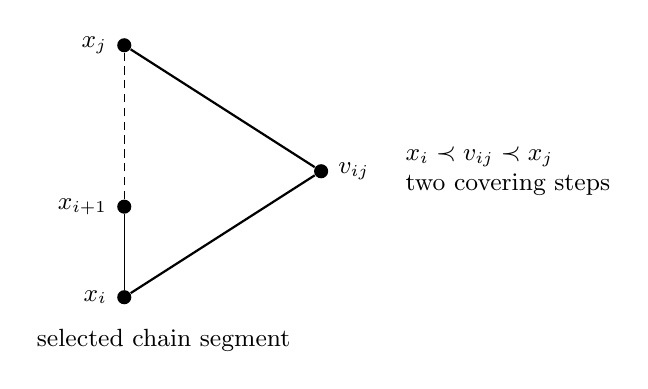
\begin{tikzpicture}[x=1cm,y=1cm,
  vertex/.style={circle,fill=black,inner sep=1.8pt},
  every node/.style={font=\small}]
\node[vertex,label=left:{$x_i$}] (lo) at (0,0) {};
\node[vertex,label=left:{$x_{i+1}$}] (mid) at (0,1.15) {};
\node[vertex,label=left:{$x_j$}] (hi) at (0,3.2) {};
\node[vertex,label=right:{$v_{ij}$}] (shortcut) at (2.5,1.6) {};
\draw (lo)--(mid);
\draw[densely dashed] (mid)--(hi);
\draw[thick] (lo)--(shortcut)--(hi);
\node[align=left,anchor=west] at (3.45,1.6)
  {$x_i\prec v_{ij}\prec x_j$\\two covering steps};
\node[align=center] at (0.5,-.55) {selected chain segment};
\end{tikzpicture}
\caption{One shortcut in a tested chain. The two thick edges are covers
in the entire subgroup interval; the selected chain on the left can
have arbitrarily many intermediate vertices and is not required to be
saturated. Fences, coatom witnesses, and the $M_{16}$ tests are omitted.
The proof compares the restrictions imposed by every short route with
those imposed by traversing a long chain.}
\label{fig:tested-chain}
\end{figure}


\begin{theorem}[Chain rigidity]\label{cls:chain-rigidity}
There is an absolute integer $B$ such that every tested chain of length
$N\geq B$ satisfies $T_a\cong T_b$.
\end{theorem}

The proof proceeds by contradiction through arbitrarily long tested
chains whose endpoint types differ.  This section gives the classification
and uniformity reductions.  Proposition~\ref{grw:remaining-paths} removes
the geometric and cross-characteristic alternatives; the proof of
Theorem~\ref{cls:chain-rigidity} is completed in Section~\ref{sec:rigidity}.
Passing to a subchain always retains the originally supplied shortcuts
and tests.  It does not assert that the subchain, with a new initial
endpoint, is a new tested chain.

\subsection{Literature inputs and maximal-step factor actions}

\begin{proposition}[Maximal-subgroup input]\label{cls:literature}
The following results are used from the classification and representation
theory of finite simple groups.
\begin{enumerate}[label=\textup{(L\arabic*)}]
\item A maximal subgroup of an almost simple classical group, not
containing its socle, is a stabilizer in one of Aschbacher's eight
geometric collections, or has an almost simple irreducible component.
The geometric collections are subspace or flag stabilizers, direct-sum
decompositions, extension-field structures, tensor products, subfield
structures, symplectic-type groups, tensor-induced decompositions, and
forms.  Graph automorphisms may interchange the relevant subspaces or
flag members; triality and exceptional graph--field automorphisms occur
only in bounded rank.  We use
\cite{Aschbacher1984} and the almost simple formulation and descriptions
in \cite[Table~1.2.A and Theorem~1.2.1, pp.~3--4]{KleidmanLiebeck1990},
with the geometric descriptions in Chapters~3--5; the connected tensor
structures and their finite fixed-point versions are also given in
\cite[Theorem~2 and Section~4(5)]{LiebeckSeitzClassical1998}.
\item The maximal subgroups of alternating and symmetric groups have
the intransitive, imprimitive, affine, diagonal, product-action, or
almost simple alternatives of the maximal-subgroup form of the
O'Nan--Scott Theorem.  The relevant formulation and all the alternatives
used here are recorded in the proof of
\cite[Proposition~3.1]{BurnessLiebeckShalev2017}.
\item For a fixed algebraic type, sufficiently general finite subgroups
lie between the derived group and the inner-diagonal group of a finite
fixed-point group.  The complementary alternative is containment in a
proper algebraic subgroup of bounded complexity.  The bounded-envelope
version permits passage to the reductive simple quotients of that
subgroup; see \cite[Theorems~0.5 and~12.3]{LarsenPink2011}.
\item A subgroup maximal in a maximal subgroup of an almost simple
group has at most five nonabelian chief factors
\cite[Proposition~8.1]{BurnessLiebeckShalev2017}.  The number refers to
chief factors, not to their simple direct factors.
\item If $[H,A]$ is a height-two interval and $A$ is alternating or
symmetric of degree at least five, it has at most eleven interior
vertices \cite[Theorem~D]{Basile2008}.  Here the entire interval is required to have height two: $H$ is
maximal in every maximal overgroup. This is the hypothesis imposed
whenever the result is used.
\item Cross-characteristic irreducible projective degrees satisfy the
Landazuri--Seitz lower bounds \cite{LandazuriSeitz1974}.  In particular,
outside bounded rank, a source of natural dimension $n$ and field parameter $q$ requires
degree at least $q^{c n}$ for an absolute $c>0$; the applicable
classical bounds are recorded in \cite[Tables~3--6]{Hasa2014}.
Above an absolute classical rank, every perfect central cover of a
finite simple classical group is a central quotient of its usual
simply connected fixed-point group, uniformly over all finite fields,
including the standard graph twists
\cite[Theorem~1.1 and p.~528]{Steinberg1981}.
The central-cover deduction and preservation of representations
are proved in Lemma~\ref{lift:finite-covers}.
After passing to that cover, defining-characteristic irreducibles
have the Steinberg highest-weight and tensor-product parametrization
\cite[Theorems~1.1 and~1.3]{Steinberg1963}, including the twisted
fixed-point groups \cite[Theorem~43]{SteinbergNotes}.
\end{enumerate}
\end{proposition}

The clauses of Proposition~\ref{cls:literature} are literature inputs.
We first control the actions on simple factors and the resulting chains
of projected cores. Numerical field and dimension estimates will enter in
Section~\ref{grw:section}, after the reduction obtained here. No classification of arbitrary subgroup
chains is assumed.

For a transitive action of a group $K$ on a factor set, with point
stabilizer $K_\omega$, a tower
$K_\omega=K_r\leq\cdots\leq K_0=K$ describes successive invariant
block systems. We call the induced coset actions of $K_{j-1}$ on
$K_{j-1}/K_j$ its \emph{action levels}. The action kernels remain in
these stabilizer groups.

\begin{proposition}[Factor actions at a maximal step]\label{cls:factor-actions}
Consider a strict labelled cover and its one-coordinate maximal subgroup
$M$ in an almost simple group, as supplied by
Proposition~\ref{frm:projection}. Mark its active nonabelian chief factor.
There are absolute positive integers $b_0,r_0$ with the following property.
\begin{enumerate}[label=\textup{(C\arabic*)}]
\item\label{cls:cat-actions}
The action on the simple factors of the marked chief factor is obtained
through at most $r_0$ transitive action levels.  Each level either has
degree at most $b_0$, or is the natural action of $A_d$ or $S_d$.
\end{enumerate}
\end{proposition}

\begin{proof}
We spell out the factor actions.  A subspace or paired-flag
stabilizer has at most a bounded number of Levi components.  A tensor
product of two spaces has two component groups.  Extension-field,
subfield, form, and almost simple cases have one, except for the
bounded low-dimensional coincidences.  A direct-sum decomposition or
a tensor-induced decomposition has the full symmetric action on its
blocks, with a possible alternating restriction from the determinant
or spinor condition.  A block contributes at most a bounded number of
simple factors; for instance an orthogonal plus-type four-space
contributes two.  Taking a point inside a block and then the block
itself accounts for this extra bounded level.  In the alternating
case, the intransitive and affine alternatives have bounded component
actions, while the imprimitive, diagonal, and product-action
alternatives have this same full block action.  Exceptional types have
bounded rank and hence bounded numbers of components.  Central,
determinant, and form quotients do not split a simple component into
more factors.  This proves \ref{cls:cat-actions}; the explicit
$\mathcal C_2$ and $\mathcal C_7$ component quotients can also be read
in \cite[proofs of Lemmas~5.4 and~5.9]{BurnessLiebeckShalev2017}.
\end{proof}

Several structural consequences of the maximal-subgroup descriptions
will be needed when we reduce to classical groups of large rank.
For a classical target and a classical active source type of sufficiently
large rank, a cover with more than one active simple factor belongs to the
geometric block or tensor cases. A soluble classical component has absolutely
bounded natural dimension: a linear group in growing dimension contains
a growing special linear simple section, and the corresponding assertion
for a form group follows from its natural hyperbolic subspaces.
For a fixed nonabelian simple type, the possible natural classical
realizations have boundedly many dimensions. Outside the bounded list
of low-order isomorphisms, its field, family, and dimension are determined
by its type; dual, form, and special-isogeny conventions add only
boundedly many choices. Finally, a geometric stabilizer has boundedly
many component slots apart from repeated blocks. Thus fixing the inactive
simple labels, repetition degrees, and bounded structural choices leaves
boundedly many possible omitted dimensions. These facts use the full
geometric stabilizers in Proposition~\ref{cls:literature}(L1), not a bound
on the orders of the components. Their numerical field and order data
will be established in Section~\ref{grw:section}.

\subsection{A uniform lemma for natural giant actions}

The shortcuts will put the relevant factor stabilizers inside one fixed
projected bottom group. We need to control their composition types and
indices simultaneously. The next two lemmas do this for bounded
stabilizer towers, including the overgroups that arise when equal-type
strips are merged.

For a finite group $H$, write $\operatorname{cf}_{\mathrm{na}}(H)$
for its set of nonabelian simple composition-factor types.  Only these
types will be bounded; the set of cyclic-prime factors need not be.

\begin{lemma}[Bounded routes]\label{cls:routes}
Fix positive integers $r,b$.  Suppose
\[
 A=H_r\leq H_{r-1}\leq\cdots\leq H_0=H
\]
and every induced action on $H_{j-1}/H_j$ is either of degree at most
$b$ or is a natural alternating or symmetric action.  There are
constants $h,c,k$, depending only on $r,b$, such that:
\begin{enumerate}[label=\textup{(\roman*)}]
\item the interval $[A,H]$ has height at most $h$;
\item the set $\{[H:U]:A\leq U\leq H\}$ has cardinality at most $k$;
\item for every such $U$, its nonabelian composition types belong to
\[
 \operatorname{cf}_{\mathrm{na}}(H)
 \cup\{A_{d-j}:A_d\in\operatorname{cf}_{\mathrm{na}}(H),\ 0\leq j\leq c\}
 \cup\mathcal E_{r,b},
\]
where $\mathcal E_{r,b}$ is a fixed finite set of types.
\end{enumerate}
The conclusions also hold for stabilizers of all invariant quotient
blocks of the action on $H/A$.
\end{lemma}
\begin{proof}
We induct on $r$.  The assertion for one step follows from primitivity
of a natural giant, or from the bounded index in the other case.
For the induction put $N=\operatorname{core}_H(H_1)$.  For an
arbitrary $U\in[A,H]$, the group $A(U\cap N)$ lies in $[A,H_1]$,
and its intersection with $N$ is $U\cap N$.  The induction hypothesis
therefore controls the intersection chain and its types.  A strict
increase in $U$ must increase $U\cap N$ or $UN/N$, since equality of
both gives equality of orders.  Furthermore
\[
 [H:U]=[H/N:UN/N]\,[N:U\cap N],
\]
and the possible second factors are a fixed multiple of the possible
indices $[H_1:A(U\cap N)]$.  Thus it remains to control the images.

If $H/N$ has bounded degree, its order is at most $b!$ and there is
nothing more to prove.  Otherwise it is $A_d$ or $S_d$, and $H_1/N$
is its natural point stabilizer.  Project the remaining route into
$H_1/N$.  A natural-giant step projects either to the same action or
to a trivial action, because it is primitive; a bounded-degree step
retains bounded degree.  Starting with the natural $A_{d-1}$ in
$H_1/N$, retain an alternating group normal in the current projected
group and supported on all but at most $r$ points.  A natural-giant
quotient either kills this alternating group, which is then retained
in the next subgroup, or maps it onto the natural alternating socle
of its image.  In the latter case equality of orders gives the same
degree, and its point stabilizer removes one supported point.
A step of bounded degree retains the alternating group once its
order exceeds $b!$.  After a step, take the union of all conjugates
of the retained support in the new subgroup.  The overlapping-support
argument in the next paragraph supplies a normal alternating group
on that union, without further loss of points.
Apart from a possible sign on the large support, the residual
quotient acts on the omitted points and has order at most $2r!$.
For $d>2r+b+10$, each step therefore loses at most one supported
point, and the terminal image contains the alternating group
supported on at least $d-r$ points.  Here the identification
of the next point stabilizer uses
$\operatorname{Aut}(A_e)=S_e$ for $e\geq7$; the degree-six exception
and all smaller first degrees are absorbed in the fixed finite
universe.  Thus we may take $c=r$ in the large-degree argument.

An overgroup of an alternating group supported on $d-c$ points has
bounded height and boundedly many possible indices.  To see this
directly, assume $d>2c+4$.  The supports of any two conjugates overlap
in at least three points, so their alternating groups generate the
alternating group on the union of their supports.  The union of
all conjugate supports is an orbit of the overgroup; its conjugate
alternating groups generate the alternating group on that orbit.
The orbit omits at most $c$ points.  Modulo the
alternating group on that orbit, the overgroup has order at most
$2c!$.  Its large simple type is therefore $A_{d-j}$ with
$0\leq j\leq c$, and its possible indices belong to the finite list
of falling factorials $(d)_j$ divided or multiplied by integers
bounded in terms of $c$.  The excluded small $d$ add only bounded
groups.  Combining this with the intersection induction proves
all three conclusions.  Invariant quotient blocks correspond
exactly to the overgroups $U$ already considered.
\end{proof}

\begin{lemma}[A common index palette]\label{cls:index-recipes}
Fix positive integers $R,b,K$.  Consider any collection of the
routes in Lemma~\ref{cls:routes}, each of length at most $R$ and
bounded degree at most $b$, such that all their natural giant
degrees belong to one set $\mathcal D$ with $|\mathcal D|\leq K$.
The union, over all groups and routes in the collection, of all
indices $[H:U]$ with $A\leq U\leq H$ has cardinality bounded by a
function of $R,b,K$.  The same holds through a bounded number of
operations, each consisting of a permitted route followed by an
arbitrary invariant quotient-block choice, with a fresh route
inside the chosen block stabilizer permitted at the next operation.
\end{lemma}
\begin{proof}
Put $d_0=2R+b+10$ and $M=d_0!$, and define the positive rational
atoms
\[
 \Gamma(\mathcal D)=
 \{u/v:1\leq u,v\leq M\}
 \cup\{(d)_j:d\in\mathcal D,\ d>d_0,\ 0\leq j\leq R\}.
\]
We claim that every index on a route of length $r$ is a product of
at most $L_r=r(r+3)/2$ atoms or their inverses.  Induct on $r$,
putting $N=\operatorname{core}_H(H_1)$ and
$B=A(U\cap N)$.  Since $U\cap N\trianglelefteq U$, we have
$A\leq B\leq H_1$ and $B\cap N=U\cap N$.  Consequently
\begin{equation}\label{cls:route-index-identity}
 [H:U]=[H/N:UN/N]\,
        \frac{[H_1:B]}{[H_1:AN]}.
\end{equation}
The image factor is bounded by $M$ when the first action is small.
Otherwise the supported alternating-group calculation in
Lemma~\ref{cls:routes} gives
\[
 [H/N:UN/N]=\frac{\varepsilon(d)_j}{t},\qquad
 0\leq j\leq r,\quad \varepsilon\in\{1,2\},\quad1\leq t\leq2j!.
\]
It therefore uses at most two atoms.  The numerator $[H_1:B]$
uses at most $L_{r-1}$ atoms by induction.

The denominator is controlled across the whole collection, not
just held fixed within one route.  Project the suffix route into
$H_1/N$.  Its degree is exactly
\begin{equation}\label{cls:route-denominator}
 [H_1:AN]=\prod_{j=2}^{r}
 [H_{j-1}N/N:H_jN/N].
\end{equation}
Under any homomorphism with kernel $C$, a natural step $L_0>L_1$
projects to the same full natural action or to a trivial action:
maximality gives $L_1C=L_1$ or $L_0$.  A bounded step keeps bounded
degree.  Thus every factor on the right of
\eqref{cls:route-denominator} is an allowed natural degree, a
bounded integer, or one, and is a single atom.  In particular no
arbitrary scalar-kernel divisor enters the denominator.
Equation~\eqref{cls:route-index-identity} gives
$L_r\leq L_{r-1}+2+(r-1)$, proving the claim.

There are at most $M^2+K(R+1)$ atoms, so the union of all index
palettes has cardinality at most
\[
 \bigl(1+2(M^2+K(R+1))\bigr)^{L_R}.
\]
Only integral values of these rational recipes occur as actual
indices.  Invariant quotient blocks correspond to the overgroups
$U$ already allowed.  If $H'$ is any such block stabilizer, apply
the argument anew to the next full route inside $H'$; it is not
necessary that $H'$ itself admit a natural-step route from $H$.
Indices multiply through a bounded number of these operations,
giving the final assertion.
\end{proof}

\begin{lemma}[Uniform active actions]\label{cls:uniform-actions}
Suppose a tested chain has $T_a\not\cong T_b$, and project at one
coordinate of the socle of $b$.  Let $H_*$ be the image of the factor
stabilizer in $a$.  Then:
\begin{enumerate}[label=\textup{(\roman*)}]
\item $H_*$ has at most five nonabelian chief factors;
\item there is one set of nonabelian types, of absolutely bounded
cardinality, which contains the types of every whole projected
stabilizer group in $H_*$ of an active factor, of an intermediate
fiber, or of an invariant quotient block used along a two-edge
shortcut, and the types of all their induced images;
\item equal-type stretches of chain vertices have absolutely
bounded length;
\item the set of ratios $m_{x_i}/m_{x_j}$, $i<j$, has absolutely
bounded cardinality after equal-type repetitions are removed.
\end{enumerate}
\end{lemma}
\begin{proof}
By Propositions~\ref{frm:strict-product} and~\ref{frm:projection}, the
starting group is a nontrivial proper coordinate product, and all
designated intersections of coatoms are saturated.  The shortcut
$a\prec v_{0N}\prec b$ projects to a two-step maximal chain in an
almost simple group.  Thus Proposition~\ref{cls:literature} gives
the five-chief-factor bound for the actual projected bottom $H_*$.
The image of the original $D$-stabilizer need not equal $H_*$ as a
group: in general $H_*$ is that image multiplied by the starting
coordinate product.  What is required is equality of the induced
active permutation actions, as follows.

For every label $z$, the equality $z=DN_z$ implies that $D$ and $z$
have the same image on $I_z$, because $N_z$ fixes its individual
simple factors.  If $I_z\to I_w$ is a product-step factor map and
$g\in z$ fixes $i\in I_w$, write $g=dn$ with $d\in D$ and
$n\in N_z$.  Then $d$ fixes $i$ and has the same action as $g$ on
the fiber over $i$.  Thus the bottom stabilizer induces the
\emph{full} local factor action at each level, not an arbitrary
subgroup of the natural giant.  This property survives the initial
projection by Proposition~\ref{frm:active-transport}.

We now account for all the shortcuts, including middles below a
proper endpoint.  An endpoint $x_j$ is reached from $b$ by the
original shortcut $b>v_{jN}>x_j$; take an empty route for $j=N$.
The first downward step is strict, because a proper subdirect group
cannot contain the nontrivial full coordinate product at the bottom.
Two strict covers give a concatenated route of length at most
$2r_0$.  A strict cover followed by an equal-type merge instead
makes the endpoint factor stabilizer an overgroup of the first
route's terminal stabilizer.

Starting at $x_j$, the middle $v_{ij}$ and the lower endpoint $x_i$
are reached by at most two further original covers.  An equal-type
operation takes an invariant quotient block.  A strict operation
supplies a fresh full local route inside the actual current
projected factor stabilizer $U\leq H_*$.  Indeed the image of the
original $D$-stabilizer lies in $U$ and already has the full local
permutation image, whereas $U$ acts through the labelled-node
stabilizer because $a$ lies below that node.  The kernel of the
original-coordinate projection centralizes that coordinate and acts
trivially on its sections.  Thus these are equal local permutation
images; no equality of the stabilizer groups themselves is needed.

The factor maps and equal-type strips respect the original $b$
coordinates.  Here is the intersection identity behind this assertion.
For labels $x\leq z$ used in a route, work modulo $F_b$ and write
\[
 x\cap N_b=P_x^{I_b},\qquad
 N_z\cap N_b=R_z^{I_b},\qquad F_z\cap N_b=Q_z^{I_b}.
\]
These product descriptions follow from saturation and
Proposition~\ref{frm:active-transport}.  Since $F_z\leq D\leq x$ and
$N_z=F_z(N_z\cap N_b)$, intersection and the quotient map give
\[
 \frac{x\cap N_z}{F_z}
 \cong \frac{x\cap N_z\cap N_b}{F_z\cap N_b}
 =\prod_{i\in I_b}\frac{P_x\cap R_z}{Q_z}.
\]
In an equal-type comparison this is the subdirect subgroup of $S_z$
whose strips describe the merge.  Because it is a full product over
$I_b$, no strip can link factors in different original coordinates:
such a link would prohibit independent elements in the two factors.
For a strict split followed by a merge inside $[x_i,x_j]$, repeat this
identity with $x_j$ as upper vertex.  The fenced endpoint comparison
makes $x_i$ saturated in those coordinates, and the strict shortcut
cover makes its middle saturated there.  Thus the merge cannot cross
those local starting fibers either.
Altogether, every required factor, fiber, and quotient-block
stabilizer uses at most four original covers, interpreted as full
local routes or quotient operations.  Four successive operations,
each with route length at most $2r_0$, give a conservative common
bound, including all intermediate block stabilizers.

We establish the type pool before the degree and index pools.  For
fixed route parameters let
\[
 \Phi(\mathcal P)=\mathcal P
\mathbin{\cup}\{A_{d-j}:A_d\in\mathcal P,\ 0\leq j\leq c,\ d-j\geq5\}
\mathbin{\cup}\mathcal E,
\]
where $c$ and the finite exceptional set $\mathcal E$ are supplied
by Lemma~\ref{cls:routes}.  If the whole current projected group has
nonabelian composition types in $\mathcal P$, that lemma puts the
types of every route prefix and every quotient-block overgroup in
$\Phi(\mathcal P)$.  This includes any kernel of the corresponding
permutation action.  Retain the original types at every iteration.
Starting with $\operatorname{cf}_{\mathrm{na}}(H_*)$, of cardinality
at most five, a bounded number of iterations gives one pool of
absolute bounded cardinality for all these projected groups.
Their induced images have no additional composition types.  This
proves (ii); it makes no claim about entire unprojected stabilizers
in the original group.

For an equal-type stretch, fix its highest vertex.  Equal-type
transport identifies all earlier vertices with strip subgroups
of that socle, whose support partitions strictly change along the
stretch.  Equal support partitions and subgroup inclusion would
force equality of orders and hence equality of subgroups, including
the diagonal twists.  The preceding coordinate compatibility
restricts these to invariant partitions of a single original
$b$-coordinate fiber.  Transitivity ensures that a strict change
appears on that chosen fiber.  All their block stabilizers are
overgroups of a single route terminal supplied by the shortcut
from $b$ to the highest vertex.  The height assertion of
Lemma~\ref{cls:routes} proves (iii).

Each full giant of large degree $d$ contributes the composition
type $A_d$ to its actual starting projected group.  Every such group is a route
prefix already covered by the preceding pool.  Hence the set
$\mathcal D$ of giant degree values occurring anywhere in these
bounded operations has absolute bounded cardinality.  The values
may be large.  Apply Lemma~\ref{cls:index-recipes} with this entire
set $\mathcal D$, and multiply indices through the bounded number
of operations.  This yields a common index palette across all the
actions, including arbitrary quotient-block choices followed by
fresh full routes.  In particular it is a union bound, not merely
a separate cardinality bound for each action.

More explicitly, put $q_i=m_{x_i}/m_b$.  The original shortcut from
$b$ to $x_i$ realizes $q_i$ as the degree on its active-factor fiber:
a strict/strict path gives a route degree, and a strict/merge path
gives a quotient-block degree.  The common recipe palette bounds
the cardinality of $\{q_i\}$.  Since
$m_{x_i}/m_{x_j}=q_i/q_j$, its quotient palette also has bounded
cardinality.  This proves (iv).
\end{proof}

\subsection{The core reduction}

\begin{lemma}[Killed layers and core gaps]\label{cls:core-gaps}
In the initial projection, consider chain vertices strictly above the
original starting vertex $a$, and write
\[
 K_i=H_*P_i,\qquad C_i=\operatorname{core}_{K_i}(H_*),
 \qquad Q_i=C_i\cap P_i,
\]
and let $R_i/Q_i$ be its active nonabelian chief factor.  For $i<j$,
the inner comparison and its killed kernel are
\[
 J_{ij}=(P_i\cap R_j)/Q_j,
 \qquad B_{ij}=(Q_i\cap R_j)/Q_j.
\]
There is an embedding $B_{ij}\hookrightarrow C_i/C_j$.
After deleting at most five nonsoluble gaps, an arbitrarily long
subchain remains on which all the $B_{ij}$, including the analogous
shortcut kernels, are soluble.  If the chain multiplicities are
equal, every endpoint inner comparison, projected to one factor of
its upper active socle, has just its active simple factor as a
nonabelian composition factor.
\end{lemma}
\begin{proof}
The exact product/core identity in
Proposition~\ref{frm:active-transport} gives, before projection,
\[
 (F_i\cap N_b)/F_b=Q_i^{m_b},\qquad
 (N_i\cap N_b)/F_b=R_i^{m_b},\qquad
 R_i/Q_i\cong T_i^{m_i/m_b}.
\]
Since $F_j\leq D\leq x_i$, we have $Q_j\leq P_i$.
Intersecting with the lower group and then with its core gives the
displayed formulas for $J_{ij}$ and $B_{ij}$.  Also $C_j\leq C_i$
and $R_j\leq P_j$, whence
\[
 C_j\cap R_j=Q_j.
\]
Thus $uQ_j\mapsto uC_j$ embeds $B_{ij}$ in $C_i/C_j$.

The $C_i$ form a decreasing chain of normal subgroups of the one
group $H_*$.  Each nonsoluble successive quotient consumes at least
one nonabelian chief factor of $H_*$.  There are at most five, by
Lemma~\ref{cls:uniform-actions}.  Cutting at these transitions
leaves at most six stretches; one is arbitrarily long.  The core
of a shortcut middle lies between the cores of its two endpoints,
so its killed layers are controlled by the same soluble quotient.
No separate bound on a collection of unrelated shortcut cores is
being assumed.

For the final assertion work with the original labelled vertices
$x_i<x_j$ and put
\[
 E=x_i\cap N_j,\qquad W=F_i\cap N_j,\qquad L=N_i\cap N_j.
\]
These subgroups are normal in $x_i$, with $F_j\leq W\leq L$.
The kernel of the conjugation action of $E$ on
$S_i=N_i/F_i$ is exactly $W$, because
$C_{x_i/F_i}(S_i)=1$.  When $m_i=m_j$, the product support map
$I_i\to I_j$ is a bijection.  Since $E\leq N_j$ fixes $I_j$,
it fixes every factor of $S_i$.  Its socle preimage is $L$, and
therefore
\[
 E/L\hookrightarrow\operatorname{Out}(T_i)^{m_j},
\]
which is soluble by Schreier's Theorem.  In the $x_j$ coordinates
write
\[
 E/F_j=P_{ij}^{m_j},\qquad W/F_j=Q_{ij}^{m_j},\qquad
 L/F_j=R_{ij}^{m_j}.
\]
Proposition~\ref{frm:active-transport} gives
$R_{ij}/Q_{ij}\cong T_i$, and the preceding embedding makes
$P_{ij}/R_{ij}$ soluble.

The killed kernel is exactly the one controlled in the initial
$b$ projection.  Indeed $N_j=F_j(N_j\cap N_b)$ and $F_j\leq F_i$
give
\begin{align}
 F_i\cap N_j&=F_j(F_i\cap N_j\cap N_b),\label{cls:killed-intersection}\\
 W/F_j&\cong
 \bigl((Q_i\cap R_j)/Q_j\bigr)^{m_b}.\label{cls:killed-kernel}
\end{align}
It is soluble on the retained stretch, so $Q_{ij}$ is soluble as
well.  Thus $P_{ij}$ has exactly its one active simple factor as a
nonabelian composition factor.  The same intersection calculation
identifies the killed kernels for either half of a shortcut.
This argument takes place in the original labelled $x_i$; it uses
neither projected quasiprimitivity nor a supplementation dichotomy
at an unlabelled bottleneck.  A shortcut middle which
still has several active factors can retain a nonabelian
factor-permutation quotient; this is not asserted to be soluble.
Its degrees are controlled by the common type pool, and it occurs
only in the split--merge case considered separately below.
\end{proof}

\begin{lemma}[Exclusion of alternating upper types]\label{cls:alternating}
For $u\in\mathcal U$ with $T_a\not\cong T_u$, the type $T_u$ is
not alternating of degree at least seven.
\end{lemma}
\begin{proof}
Project the strict comparison from $a$ to $u$ using
\ref{cls:test-alternating}.  The bottom is a full product and an
intersection of coatoms.  The coatoms and their intersection $c_u$
are saturated, so Proposition~\ref{frm:projection} carries the entire
interval $[c_u,u]$ to an $M_{16}$ interval ending at an almost simple
group with socle $T_u$.  For an alternating socle of degree at least
seven that group is alternating or symmetric, contradicting
Proposition~\ref{cls:literature}.  The exceptional automorphisms in
degree six concern only bounded-order types.
\end{proof}

\subsection{Why bounded rank cannot support a long strict chain}

The bounded-rank argument needs a normalized subfield group, rather
than just a numerical resemblance between two field sizes.  We give
the details, including the automorphisms of the almost simple ambient
group.

\begin{lemma}[Bounded envelopes]\label{cls:envelopes}
Fix a connected adjoint simple algebraic type $\Phi$.  There is a
constant $c_\Phi$ such that a finite subgroup $P$ of an algebraic
group $X$ of type $\Phi$ has one of the following descriptions.
\begin{enumerate}[label=\textup{(\roman*)}]
\item For a Frobenius map $F_0$,
\[
 E=(X^{F_0})'\leq P\leq X^{F_0},
\]
where $E$ is simple.
\item Every nonabelian composition factor of $P$ of order greater
than $c_\Phi$ is of Lie type in the characteristic of $X$, with
algebraic dimension strictly less than $\dim X$.  The total number
of nonabelian composition factors, counted with multiplicity, is at
most $c_\Phi$.
\end{enumerate}
In particular, the ranks of nonabelian simple sections of finite
groups of Lie type of rank at most $R$ are bounded by a function of
$R$; simple sections of bounded order are included in this bound.
\end{lemma}
\begin{proof}
Apply \cite[Theorem~0.5]{LarsenPink2011}.  Outside (i), $P$ lies in
a proper algebraic subgroup $B<X$ from a fixed constructible family.
Apply \cite[Theorem~12.3]{LarsenPink2011} to that family.  It supplies
an envelope $H\leq B$, with $P\leq H$, whose connected reductive
quotient has simple adjoint factors $X_1,\ldots,X_t$ such that the
image $L_i$ of $P\cap H^\circ$ satisfies
\[
 E_i=(X_i^{F_i})'\leq L_i\leq X_i^{F_i},
\]
with $E_i$ simple.  Each $\dim X_i\leq\dim H^\circ<\dim X$.
The kernel of the map from $H^\circ$ to the product of its simple
adjoint quotients is soluble: it is an extension of the unipotent
radical by the full center of the connected reductive quotient.
That center can be disconnected, but is abelian.  If $L$ is the image of $P\cap H^\circ$
in $\prod_i L_i$, then $L'$ is a subdirect subgroup of
$\prod_iE_i$, because each $L_i/E_i$ is abelian.  The subdirect
product Lemma makes $L'$ a product of full diagonals.  Its simple
factors are therefore among the $E_i$, counted at most once per
position.  There are at most $\dim X/3$ positions.

The component bound in \cite[Proposition~1.4]{LarsenPink2011} bounds
$|H/H^\circ|$ throughout this constructible family.  Its contribution
has bounded order and bounded composition length.  This proves (ii).
Applying the same argument to every subgroup of a finite group of
rank at most $R$ proves the last assertion: the ambient algebraic
dimensions range over a finite set, and the finitely many small
orders and characteristics in the exceptional alternative are
absorbed in a function of $R$.
\end{proof}

\begin{lemma}[Normalized subfield steps]\label{cls:subfields}
Fix an adjoint simple type $\Phi$.  Let $T=(X^F)'$ be simple,
$T\leq A\leq\operatorname{Aut}(T)$, and let $M<A$ be maximal with
$T\not\leq M$.  Suppose that $P=M\cap T$ is in alternative (i) of
Lemma~\ref{cls:envelopes}, and that the parameter of $F_0$ is large
enough in terms of $\Phi$.  Then $F=F_0^r$ for a prime $r$.
Every element of $M$ normalizes the derived fixed-point groups for
all intermediate powers of $F_0$.
\end{lemma}
\begin{proof}
First, the pointwise centralizer of $E=(X^{F_0})'$ in
$\operatorname{Aut}_{\rm alg}(X)$ is trivial when the field parameter
is sufficiently large.  Indeed the fixed groups $X^a$, for nonidentity
algebraic automorphisms $a$, form a constructible family of proper
closed subgroups: take the equalizer of the action and projection
maps over the finite-type algebraic automorphism group, remove the
identity section, and stratify.  Now use
\cite[Proposition~3.5]{LarsenPink2011}.

Here is the isogeny calculation needed to include field and exceptional
graph operations.  Let $\mathcal I(X)$ be the group of bijections of
$X(\overline{\mathbb F}_p)$ generated by self-isogenies and their
inverses.  The isogeny Theorem
\cite[Theorem~6.1.16(1) and Proposition~6.1.13(2)]{Conrad2014}
gives a homomorphism
\[
 \nu:\mathcal I(X)\longrightarrow\mathbb Z,
 \qquad\ker\nu=\operatorname{Aut}_{\rm alg}(X).
\]
For completeness, after fixing a Borel pair, a self-isogeny permutes
the simple roots by $\pi$ and raises their parameters to powers
$p^{e_i}$.  Use the row-coroot convention
$C_{ij}=\langle\alpha_j,\alpha_i^\vee\rangle$ for the Cartan
matrix.  The compatibility condition is
\[
 p^{e_j}C_{ij}=p^{e_i}C_{\pi(i)\pi(j)}.
\]
The labeled undirected Coxeter diagram is preserved.  Unless a
multiple edge is reversed, connectedness forces all $e_i$ equal.
An edge reversal is possible only for $B_2,F_4$ in characteristic
two, or $G_2$ in characteristic three.  The exponents on the two root
lengths then differ by one.  Thus every self-isogeny is $a\theta^m$,
where $a$ is algebraic, $m\geq0$, and $\theta=F_p$ except in those
three cases, when $\theta^2=F_p$; see also
\cite[Remark~6.2.10]{Conrad2014}.  Root-group constants are absorbed
by the algebraic automorphism, using the pinned uniqueness in the
isogeny Theorem.  Conjugation by $\theta$ preserves algebraic
automorphisms, so the same normal form holds with $m\in\mathbb Z$
in $\mathcal I(X)$.  Inseparability degree proves uniqueness of $m$,
and $\nu(a\theta^m)=m$ is the asserted homomorphism.  Positive
$\nu$ gives a Frobenius map: Lang--Steinberg removes its inner
factor, leaving a positive diagram--field map
\cite[Proposition~2.7(i), p.~435]{LiebeckSeitzClassical1998}.
Its field parameter
is $p^{\nu}$, or $p^{\nu/2}$ in the three exceptional cases.

Let $C_E\leq\mathcal I(X)$ fix $E$ pointwise.  The preceding
centralizer observation makes $\nu|_{C_E}$ injective.  Its image is
a nonzero subgroup of $\mathbb Z$, since it contains $\nu(F_0)$.
Thus $C_E=\langle F_1\rangle$ for a Frobenius map $F_1$, and
$F_0=F_1^b$ for some $b\geq1$.  Put $d=\dim X$ and let $q_0$ be
the parameter of $F_0$.  The fixed-point order bounds and bounded
diagonal index in \cite[Theorem~3.4(b),(d)]{LarsenPink2011} give
\[
 \frac{(q_0-1)^d}{z_\Phi}
 \leq |E|\leq |X^{F_1}|
 \leq c_\Phi q_0^{d/b}.
\]
Enlarging $c_\Phi$ includes the finitely many possibilities for the
parameter of $F_1$ below four.  For sufficiently large $q_0$, this
forces $b=1$.  Consequently $C_E=\langle F_0\rangle$.  Since $F$
fixes $E$, it follows that $F=F_0^r$ with $r>0$.

The quotient $P/E$ is abelian and $E$ is perfect, so $P'=E$.
Every $m\in M$ therefore normalizes $E$.  The finite automorphism
Theorem \cite[Theorems~30 and~36]{SteinbergNotes} lifts $m$ to an
element $\widetilde m\in\mathcal I(X)$.  The commutator
$\widetilde mF_0\widetilde m^{-1}F_0^{-1}$ has $\nu=0$ and fixes
$E$ pointwise.  It is therefore the identity.  Thus $m$ normalizes
$E_e=(X^{F_0^e})'$ for every divisor $e$ of $r$.

We have $r>1$, since $r=1$ would give $T\leq M$.  If $r$ were
composite, choose $1<e<r$ dividing $r$.  Fixed-point order estimates,
after increasing the original field threshold, give
$E_e\not\leq P$ and $1<E_e<T$.  Hence
\[
 M<ME_e\leq N_A(E_e)<A.
\]
The last inequality follows because $T$ is simple and cannot
normalize a nontrivial proper subgroup of itself.  This contradicts
maximality and proves that $r$ is prime.
\end{proof}

\begin{lemma}[Bounded-rank chains]\label{cls:bounded-rank}
For every $R$ there is $b(R)$ such that at most $b(R)$ distinct Lie
types of rank at most $R$ occur in a tested chain after the alternating
exclusion.  In an arbitrarily long family of such chains with distinct
types, one may therefore require the ranks of all retained endpoints
and all their shortcut middles to exceed any prescribed constant.
\end{lemma}
\begin{proof}
Consider a subsequence of distinct endpoint types of ranks at most
$R$.  A lower simple type is a section of each later one by
Proposition~\ref{frm:equal-transport}; in particular their orders increase strictly.
Remove the boundedly many types below the order thresholds of
Lemma~\ref{cls:envelopes}, for the finitely many relevant algebraic
types.  Every two-edge shortcut has intermediate types of rank
bounded in terms of $R$, by the last assertion of that lemma.
Increase the threshold accordingly.  On each strict cover read
downwards, the characteristic is then unchanged and the algebraic
dimension does not increase.  The only case of equal algebraic
dimension is the sufficiently general alternative.  An equal-type
cover changes neither characteristic nor dimension.

There are finitely many possible dimensions and algebraic families.
If the subsequence were arbitrarily long, it would have an
arbitrarily long further subsequence with one dimension and family.
On every prescribed two-edge shortcut between its endpoints the
dimension cannot drop.  Each strict cover is therefore a normalized
prime subfield step by Lemma~\ref{cls:subfields}; a possible equal-type
cover contributes no field change.  With one fixed family at the
endpoints, the conversion between its usual exponent $f$ and the
Frobenius parameter exponent cancels.  Thus, for every $i<j$,
\[
 f_j/f_i\in\mathbb Z_{>1},\qquad \Omega(f_j/f_i)\leq2,
\]
where $\Omega$ counts prime factors with multiplicity.  Four
successive endpoints would give
\[
 \Omega(f_4/f_1)=\sum_{i=1}^3\Omega(f_{i+1}/f_i)\geq3,
\]
a contradiction.  All discarded sets and pigeonhole choices have
bounds depending only on $R$, proving the first assertion.

For any desired rank threshold, remove the boundedly many endpoints
below a sufficiently larger threshold.  If a remaining shortcut
middle had bounded rank, its lower endpoint, being a simple section
of it, would have rank bounded by Lemma~\ref{cls:envelopes}.  The
larger threshold was chosen to exclude this.  Arbitrarily long
chains remain, proving the second assertion.
\end{proof}

\subsection{The configuration passed to the growth argument}

\begin{proposition}[Reduction to classical one-factor comparisons]
\label{cls:reduction}
If Theorem~\ref{cls:chain-rigidity} is false, then for every $s$ and
$R$ there is a retained chain of at least $s$ vertices, with all its
original two-edge shortcuts and normal-group tests, such that:
\begin{enumerate}[label=\textup{(\roman*)}]
\item all endpoint types are distinct classical types; their ranks,
and the ranks of all shortcut middle types, exceed $R$;
\item all endpoint multiplicities are equal.  Thus each comparison,
projected to one upper active coordinate, has one active simple
factor;
\item the killed kernels of all endpoint and shortcut comparisons
are soluble.  Every endpoint inner comparison has exactly its one
active simple factor as a nonabelian composition factor;
\item there is a pool of absolutely bounded cardinality containing
all nonabelian simple types in every projected active-factor and fiber
stabilizer in the fixed $H_*$, and in their induced images, used in
these comparisons.  No assertion concerns the entire unprojected
original stabilizers.  The splitting multiplicities
and invariant-block indices have boundedly many possible values;
\item each shortcut is either two strict steps, both with one
active simple factor and all other inner composition factors
soluble, or a strict split followed downwards by an equal-type
merge.  The latter is geometric.  In geometric steps the inactive
dimensions have boundedly many possible values once their simple
labels and bounded structural choices are fixed; when all inactive
components are soluble these dimensions are absolutely bounded.
\end{enumerate}
All bounds described as absolute are uniform over the original
groups.  This proposition introduces no new lattice tests at the
retained bottom.
\end{proposition}
\begin{proof}
Take counterexamples of lengths tending to infinity, retaining the
original endpoints initially.  A lower simple type is a section of
an upper one, so equality of the endpoint types of a segment forces
equality throughout that segment.  Lemma~\ref{cls:uniform-actions}
bounds the lengths of these equal-type stretches.  Choose one
vertex from each stretch and discard the original initial stretch.
There are arbitrarily many remaining vertices, and none has the
type of the original $a$.  Their shortcut middles are above a
retained lower vertex, so also cannot have type $T_a$.
Lemma~\ref{cls:alternating} now excludes all large alternating
types at both endpoints and middles.  Sporadic groups and all other
bounded-order coincidences form a finite list.  Bounded-rank Lie
types can be removed using Lemma~\ref{cls:bounded-rank}.  This gives
(i), with arbitrarily large minimum rank.

All later coordinate projections still use the original tests.
For a retained upper endpoint or middle $u$, condition
\ref{cls:test-alternating} applies to $a<u$, with
$T_a\not\cong T_u$.  Proposition~\ref{frm:projection}, with
original lower vertex $a$, gives $H_a\cap T_u=P_a$.  A retained
vertex $z$ saturated in these coordinates then has
\[
 K_z=H_aP_z,\qquad K_z\cap T_u=P_z,
\]
because $P_a\leq P_z$.  Saturation for a distinct-type endpoint
comparison comes from its fence, and saturation at a strict
shortcut cover comes from its coatom status.  Thus the required
inner-intersection identity never relies on inheriting a local
coatom-meet representation from the global one below $b$, or on a
new test at a retained bottom.

Use the common cardinality bound on ratios in
Lemma~\ref{cls:uniform-actions} to color pairs by $m_i/m_j$.
Finite Ramsey gives an arbitrarily long homogeneous subchain.
On a homogeneous triple the common ratio $t$ satisfies $t^2=t$;
since $t>0$, it is one.  This proves (ii).  Next apply
Lemma~\ref{cls:core-gaps} in the original fixed projection: deleting
the at most five nonsoluble transitions leaves an arbitrarily long
stretch.  All shortcut cores between its endpoints lie in the
corresponding soluble gap.  Passing to any later active coordinate
takes subgroups and images of these soluble killed kernels, and
hence preserves solubility.  Lemma~\ref{cls:core-gaps} and
Proposition~\ref{frm:active-transport} give (iii).

The common type pool and index bounds are precisely
Lemmas~\ref{cls:uniform-actions} and~\ref{cls:index-recipes}; none of
these bounds counts abelian factors.  They remain valid under all
the preceding thinning, giving (iv).

Read a shortcut downwards from its upper endpoint.  Its first
cover cannot be a proper subdirect merge, because the lower endpoint
is a nontrivial full product.  If both covers are strict, their
positive integral splitting multiplicities multiply to the endpoint
ratio one.  Both are therefore one.  Their killed kernels are
soluble by (iii), and their tails are soluble by
Proposition~\ref{frm:active-transport}.  If the second cover is an
equal-type merge, the first must split; the only unbounded-rank
maximal-subgroup cases with such an active split are the geometric
block and tensor cases described after
Proposition~\ref{cls:factor-actions}.  The
merge stays inside each original upper coordinate.  Its possible
indices are already covered by (iv).

The inactive nonabelian labels in a shortcut belong to the pool in
(iv). To see this, write its local inner group as $P\trianglelefteq K$,
with soluble killed kernel $Q$ and active chief factor $R/Q\cong T^a$.
The faithful conjugation argument in
Proposition~\ref{frm:active-transport} gives
$P/Q\hookrightarrow\operatorname{Aut}(T^a)$. The kernel of the
factor-permutation map on $P/R$ lies in
$\operatorname{Out}(T)^a$ and is soluble. Since $P$ is normal in $K$,
its permutation image is normal in the full local permutation image.
Lemma~\ref{cls:uniform-actions} identifies that full image with an
image of one of the projected stabilizers counted in (iv). Its normal subgroup
therefore has its nonabelian composition types in the same pool. Thus
all nonabelian composition types outside the active chief factor
$R/Q$ lie in this pool. The active type $T$ can still vary along the chain.

Apply now the structural observations following
Proposition~\ref{cls:factor-actions}. There are boundedly many choices
of inactive simple labels by (iv), and the repetition indices also
have boundedly many values. The resulting omitted dimensions
therefore have boundedly many possible values. When all inactive
components are soluble, their individual natural dimensions are
absolutely bounded. This proves (v) and all the assertions passed
to the next section.
\end{proof}

\section{Fields, indices, and growth along shortcuts}
\label{grw:section}

We continue the reduction of Theorem~\ref{cls:chain-rigidity}, starting
with the configurations supplied by Proposition~\ref{cls:reduction}.
Their distinct classical endpoint types have arbitrarily large rank,
their multiplicities agree, and their killed kernels are soluble.
We now compare the numerical restrictions imposed by a two-edge shortcut
with the growth obtained by traversing several successive comparisons.
The three quantities are field exponents, natural dimensions, and inner
order quotients. We first establish the maximal-step estimates needed
for these comparisons. They will exclude wholly geometric paths and
characteristic crossings, leaving common-field paths with quadratic
dimension growth and controlled inner order.

Write $z_0<\cdots<z_\ell$ for the retained original vertices, in their
original order, and abbreviate $F_i=F_{z_i}$, $N_i=N_{z_i}$,
$T_i=T_{z_i}$, $m_i=m_{z_i}$, and $I_i=I_{z_i}$. The common
bottom $D$ and lower endpoint $a$ remain those of the original tested
chain; every shortcut and normal-group test is inherited from it.
Write
\[
 T_i=T_i(q_i),\qquad q_i=p_i^{f_i},\qquad n_i=\dim V_i,
 \qquad a_i=|T_i|.
\]
Here $V_i$ is the natural simple module. In characteristic two the
type $B_r$ parameter is $n_i=2r$, using its simple symplectic natural
quotient. For a unitary group the parameter is $q_i=p_i^{f_i}$,
although its natural matrix field is $\mathbb F_{q_i^2}$.
Put $\epsilon_X=2$ for a unitary type and $\epsilon_X=1$ otherwise,
so the natural matrix field has degree $\epsilon_Xf_X$ over its
prime field. We retain this conversion for restriction of scalars;
twisted-tensor steps will have the exact usual-field relation
$f_s=b f_t$.

For each $i<j$ choose the prescribed two-edge shortcut. We write its
ascending steps as $B_{ij},A_{ij}$ and its intermediate simple label as
$Y_{ij}$; a prime denotes an intermediate parameter. The letters $A_{ij}$
and $B_{ij}$ denote steps, not subgroups. On an individual ascending
step, subscripts $s,t$ denote source and target parameters.

All uses of ``arbitrarily long'' below have the same quantifiers: for
every integer $s$ there are such configurations with at least $s$ chain
vertices, and their minimum rank can be required to exceed any prescribed
constant. A finite coloring followed by finite Ramsey preserves this
property. So does retaining every $d$th vertex for a fixed $d$. Constants
in this section are independent of the configuration and of its length.
An explicitly mentioned pool of parameter values may depend on the
configuration, but its cardinality has a uniform bound.

\subsection{Numerical structure of classical maximal steps}

The factor actions needed for the whole-chain reduction were proved in
Proposition~\ref{cls:factor-actions}. We now derive the field, dimension,
and order estimates from the maximal-subgroup descriptions in
Proposition~\ref{cls:literature}. The proofs retain the actual finite
normalizers, since their field actions will enter both the growth
argument and the later constituent calculation.

\begin{proposition}[The maximal-step catalogue]\label{cls:catalogue}
Consider a strict labelled cover and its one-coordinate maximal subgroup
$M$ in an almost simple group with socle $T$, as supplied by
Proposition~\ref{frm:projection}.  Mark its active nonabelian chief factor.
The non-geometric irreducible category below means that its simple
source acts absolutely irreducibly on the ambient natural module
and that the maximal subgroup is outside all geometric collections,
in particular the subfield collection.  All growing-rank assertions
refer to growing \emph{source} rank.
There are absolute constants $C,c>0$ with the following properties.
\begin{enumerate}[label=\textup{(C\arabic*)},start=2]
\item\label{cls:cat-geometric}
For unbounded-rank classical active types, a geometric
defining-characteristic step changes natural dimension by taking a
subspace or quotient, a repeated natural module, a tensor product, or
restriction of scalars.  Subfield steps leave natural dimension
unchanged and multiply the field exponent by a prime.  An
extension-field step, read upwards from the active factor, has
\begin{equation}\label{grw:matrix-field-convention}
 n_t=b n_s,\qquad
 \epsilon_s f_s=b\epsilon_t f_t,
 \qquad f_t=\frac{\epsilon_s}{b\epsilon_t}f_s,
\end{equation}
where $b$ is the prime degree between natural matrix fields.
A twisted-tensor step has
\begin{equation}\label{grw:twisted-field-convention}
 n_t=n_s^b,\qquad f_s=b f_t,
\end{equation}
exactly; here $b$ is prime, after bounded source-rank cases are
removed.  All other changes of field exponent
belong to a fixed finite set of positive rational factors.
\item\label{cls:cat-inactive}
If there is one active simple component and the other geometric
components are soluble, their natural dimensions are absolutely
bounded.  The active dimension in a subspace case is comparable with
the ambient dimension; a totally singular summand and its dual may
represent the same active component twice.  A nontrivial parabolic
radical in these cases has order between $q^{c n_t}$ and $q^{C n_t^2}$.
For a fixed ambient group, once the active slot, other component
dimensions, and the bounded flag/form choices are fixed, there are
boundedly many possible orders of the full inner stabilizer divided by
the order of its active simple factor, with multiplicity included.
\item\label{cls:cat-symplectic}
A symplectic-type step of unbounded active rank is
cross-characteristic.  Its source is symplectic or orthogonal over a
prime field of order $r$, of natural dimension $2d+O(1)$, and its
target natural dimension is $n_t=r^d$.  If $P=M\cap T$, then
\[
 c n_t^2\leq |P|/|T_s|\leq C n_t^2.
\]
Its target field exponent is at most $|T_s|^C$.
\item\label{cls:cat-nonlinear}
After the twisted-tensor case in
\ref{cls:cat-geometric} is separated off, a defining-characteristic almost simple
irreducible step has a single nonzero restricted, nonnatural
Frobenius digit, up to a common Frobenius twist.  This restricted
module may have further tensor factors in a very special
characteristic.  Its dimension is at least $c n_s^2$.  Its source and target field
exponents differ by a rational factor from a fixed finite set.
Natural, dual-natural, and natural-size special-isogeny representations
are included among the geometric cases instead.
\item\label{cls:cat-cross}
For a cross-characteristic almost simple step,
\[
 q_s^{c n_s}\leq n_t\leq |T_s|^C,
 \qquad f_t\leq |T_s|^C.
\]
The upper degree bound also holds in defining characteristic.
For this and the preceding irreducible case, the homomorphism from the
ambient automorphism normalizer of the source simple group to its
automorphism group has kernel of absolute bounded order.  In
particular, a subgroup of that normalizer has order at most
$C$ times the order of its induced automorphism group of the source.
\end{enumerate}
\end{proposition}

\begin{proof}
For the dimension and field statements, take the full stabilizers of
the indicated structures.  On a nondegenerate direct summand the
active group has its natural module; on a totally singular summand
the dual summand has the contragredient module.  A tensor stabilizer
acts as the tensor product of the component natural modules.
Restriction of scalars multiplies dimension by its degree $b$ and
gives $\epsilon_s f_s=b\epsilon_t f_t$ for the natural matrix
fields.  For example, the mixed $\operatorname{GU}_m(q)$ row in
$\operatorname{Sp}_{2m}(q)$ has $b=2$ and equal usual exponents,
since $\epsilon_s=2$ and $\epsilon_t=1$.  It is a restriction of
scalars, with a direct sum after scalar extension, and is not a
twisted-tensor row.  A subfield inclusion changes only the field.
If an ordinary field degree were composite, its proper intermediate
field structure would be preserved by the normalizer, contradicting
maximality.  The classical stabilizer descriptions with prime degree
are given explicitly in
\cite[proofs of Lemmas~5.5 and~5.7]{BurnessLiebeckShalev2017}.
Unitary conjugation and the diagram maps have bounded order, which
accounts for the permitted bounded ratios in the remaining field
operations.  The
twisted-tensor assertion is proved separately in
Lemma~\ref{cls:twisted-tensor} below.

The only soluble classical component groups have bounded natural
dimension: a linear group in growing dimension contains a growing
special linear simple section, and the corresponding assertions for
the form groups follow by their natural hyperbolic subspaces.
Thus the omitted dimensions in a one-active-component subspace or
tensor stabilizer are bounded.  The explicit block description of a
parabolic gives a radical of order $q^e$, with $e\leq Cn_t^2$ and
$e\geq c n_t$ whenever that radical is nontrivial in the retained
large-rank cases.  For example, the linear radical attached to a
$k$-space has exponent $k(n_t-k)$; the symplectic and orthogonal
exponents count the off-diagonal blocks subject to one symmetric or
alternating relation.  The smallest nonzero retained exponent is
linear in $n_t$.  The other factors are the displayed classical
groups and scalar groups.  Consequently their orders are determined
by the dimensions, field, form signs, and the bounded choices of
interchanged flags.  Intersecting the full stabilizer with the ambient
socle adds only its prescribed determinant or spinor condition; it
does not introduce a freely chosen subgroup of a scalar group.  This
proves \ref{cls:cat-inactive}.

For a symplectic-type normalizer put $N=n_t=r^d$, and let $W$ be
the projective image of its normal $r$-group, of order $r^{2d}$.
The full inner-normalizer rows, including their minimal-field
conditions, are given in
\cite[Section~2.2.6, pp.~70--71, Table~2.9]{BrayHoltRoneyDougal2013}.
Their small exceptions disappear on retaining $d\geq4$.
Ordinary linear conjugation fixes scalars pointwise, so it preserves
the nondegenerate scalar commutator pairing
$W\times W\to\mu_r$.  Moreover the projective linear centralizer
of $W$ is $W$: a centralizing operator twists the representing
matrices by a character of $W$, that character is implemented by
an element of $W$ through the pairing, and the remaining centralizer
is scalar by irreducibility.

In the linear and unitary rows, the normal group is an exponent-$r$
extraspecial group for odd $r$, and a central product
$C_4\circ2^{1+2d}$ for $r=2$.  In both cases the ordinary projective
normalizer has quotient $\operatorname{Sp}_{2d}(r)$ on $W$.
Indeed every symplectic change of generators lifts to a center-fixing
automorphism and is implemented by the irreducible representation
with its specified central character.  For $r=2$, multiplying a
generator by the central element of order four restores its required
square; thus a square form attached to a pure extraspecial subgroup
is not an invariant of this scalar-extended normalizer.
In the unitary case an implementing operator preserves the Hermitian
form up to a multiplier, which is removed by a scalar using the
surjective finite-field norm.
The standard tensor generators of $W$ have determinant one: for odd
$r$ this holds for the cyclic shift and diagonal root-of-unity
generators, and for $r=2$ their determinants are
$(-1)^{2^{d-1}}=1$.  The map from this normalizer to the abelian
quotient of the projective linear or unitary group by its simple
socle therefore factors through $\operatorname{Sp}_{2d}(r)$.
That group is perfect in the retained range, so the map is trivial.
Hence the full ordinary projective normalizer is already the inner
intersection $P$.  Quotienting by the entire ambient scalar center
leaves kernel exactly $W$, and
\[
 P/W\cong\operatorname{Sp}_{2d}(r),\qquad
 |P|/|T_s|=(2,r-1)N^2.
\]
This uses the quotient, without requiring the extension to split.

The pure symplectic and orthogonal form rows have $r=2$.
Here the extraspecial square form is invariant.  The cited inner
rows give $P/W=O_{2d}^{\varepsilon}(2)$ or
$\Omega_{2d}^{\varepsilon}(2)$, with active simple group
$T_s=\Omega_{2d}^{\varepsilon}(2)$ and index at most two.
These are the inner rows after the determinant and spinor conditions;
the scalar kernel of the natural cover is removed in $W$.
Consequently $N^2\leq |P|/|T_s|\leq2N^2$ in every retained row.
There is no extra factor from $r-1$ or the ambient field exponent.

The target-field bound uses the minimal-field condition of the
maximal row.  For odd $r$, the degree
$e=\operatorname{ord}_r(p)$ divides $r-1$; the usual target exponent
is $e$ in the linear row and $e/2$ in the unitary row.
The binary and pure form rows have usual exponent one.
Thus $f_t\leq\max(1,r-1)\leq |T_s|$.
The representation characteristic is different from $r$, and the
active source is over the prime field of order $r$.
This proves \ref{cls:cat-symplectic}.

For an absolutely irreducible representation of a central cover
$\widetilde T_s$, the dimension is at most
$|\widetilde T_s|^{1/2}$: the square of each simple-module dimension
is bounded by the dimension of the group algebra.  The field-of-definition bound can be obtained directly, including in
modular characteristic.  For a finite group $K$ in characteristic $p$,
there are at most $|K|$ absolute simple module types, by the semisimple
quotient of its group algebra.  Frobenius permutes these types, so an
absolute simple representation has a Frobenius orbit of length
$a\leq |K|$.  An isomorphism with its $p^a$-Frobenius twist descends the
representation to $\mathbb F_{p^a}$: choose a finite field containing
its matrices and an intertwiner, scale the intertwiner to have norm
one, and apply matrix Hilbert's Theorem~90.  The scalar norm adjustment
is possible because finite-field norms are surjective.  Apply this
with $K=\widetilde T_s$.  The Schur multipliers of the
large classical groups have order at most a polynomial in $|T_s|$;
the finitely many exceptional multipliers do not change the bound.
Forms cost an extension of degree at most two.  Maximality outside
the subfield collection makes these bounds applicable to the target
field itself.  For the cross-characteristic lower bound, the
classical tables in \cite[Section~3, Tables~3--6]{Hasa2014} give
degree at least $q_s^r/3$ once the source rank $r\geq6$, including
the smaller Weil degrees.  Their excluded families have bounded
rank.  As $n_s\leq2r+1$, this is at least $q_s^{n_s/4}$ after
increasing the rank threshold.  This proves the numerical assertions
of \ref{cls:cat-cross}.

For the defining-characteristic quadratic bound, use
\cite[Theorem~5.1 and Table~2]{Luebeck2001} in rank $r>11$.
Modules outside that table have dimension greater than $r^3/8$
in type $A$, and greater than $r^3$ in types $B,C,D$.
Every listed nontrivial, nonnatural, nondual degree is at least $r^2/2$.
Consequently the retained restricted module has dimension at
least $r^2/2\geq n_s^2/10$.  Type $B$ in characteristic two is
read through its type-$C$ natural simple quotient, as in our
parameter convention; the natural-size special-isogeny cases are
already assigned to geometry.

A single occupied ordinary Frobenius digit has full source period:
any shift strictly between zero and $f_s$ moves it to a different
position in the unique finite restricted label.  Returning through
$f_s$ applies at most the bounded diagram operation.  An internal
tensor decomposition of that digit changes neither its occupied
position nor this uniqueness argument.  Thus the minimal scalar
field degree is $f_s$ times one of the bounded diagram periods.
The matrix degree is separately $\epsilon_t f_t$.  The
form-compatible minimal-field argument in
Lemma~\ref{cls:normalizer} bounds the ratio of this matrix degree
to the minimal degree outside the geometric collections.
This gives the fixed finite rational set of usual exponent ratios
and proves \ref{cls:cat-nonlinear}.
Lemma~\ref{cls:normalizer} below supplies
the final normalizer assertion.
\end{proof}

\begin{lemma}[Irreducible normalizers]\label{cls:normalizer}
In a non-geometric absolutely irreducible step of
Proposition~\ref{cls:catalogue}, let $Y$ denote the simple source
inside the ambient projective classical group $T$.  In particular,
the maximal subgroup is not in a subfield collection.  Then
\[
 \bigl|\ker\bigl(N_{\operatorname{Aut}(T)}(Y)
       \longrightarrow\operatorname{Aut}(Y)\bigr)\bigr|\leq C
\]
for an absolute $C$.  Moreover
$|\operatorname{Out}(Y)|\leq C n_Y f_Y$ for a large-rank classical
source with parameters $(n_Y,p^{f_Y})$.
\end{lemma}
\begin{proof}
Lift the irreducible projective representation to the perfect central
cover of $Y$.  A projective linear element centralizing its image
commutes with that representation up to a linear character of the
perfect cover, hence commutes exactly.  Schur's Lemma makes it scalar,
so it disappears projectively.

If a semilinear element in this kernel has scalar-field action $\sigma$,
the representations $\rho^\sigma$ and $\rho$ are isomorphic.  If
$\sigma$ has order $a$ on the scalar field $E$, its intertwiner $A$
satisfies
\[
 A\sigma(A)\cdots\sigma^{a-1}(A)=cI,
 \qquad c\in E^{\sigma,*}.
\]
Surjectivity of the scalar norm adjusts $A$ so that the product is
one; matrix Hilbert's Theorem~90 then gives a model over $E^\sigma$.
An invariant bilinear form is a line defined by linear equations
over the minimal field, and invariant quadratic-form coefficients
satisfy linear equations there as well.  In characteristic two,
two invariant quadratic forms with the same polarization differ
by the square of an invariant linear form.  Absolute irreducibility
makes that difference zero, so the prescribed quadratic form itself
descends up to scalar.  Matching finite-field form classes costs at
most a quadratic extension.  For a unitary group the involution on
the minimal field is either nontrivial, giving Hermitian descent
and surjective norms, or trivial, giving a preserved bilinear
structure and hence a geometric form case.  A larger field period would
therefore provide a proper subfield structure normalized by the
whole irreducible normalizer, contrary to this step being outside the
subfield collection.

To justify the assertion about the whole
normalizer, put an absolutely irreducible model over its minimal
field $E_0$.  A normalizing matrix intertwines this model with the
model obtained by a source automorphism and a field automorphism;
both have entries in $E_0$.  The intertwining equations therefore
have coefficients in $E_0$.  Their solution space over the algebraic
closure is one-dimensional by absolute irreducibility.  It consequently
has a nonzero $E_0$-rational solution, necessarily invertible.  Up to a
scalar, the normalizer thus preserves the projective $E_0$-structure.
The same argument applies after dualizing in a graph component, and
the uniqueness of the invariant form gives the already allowed
quadratic extension.  A graph operation contributes at most another
factor of two in unbounded rank.  This bounds the kernel independently
of the ambient field degree.

Finally the diagonal, field, and graph
description of automorphisms gives respectively factors at most
$n_Y$, $f_Y$, and an absolute constant in the outer group.
\end{proof}

Twisted tensor subgroups and their normalizers were studied in detail by
Schaffer \cite{Schaffer1999}; the algebraic and finite tensor structures
used here are those of \cite[Section~4(5)]{LiebeckSeitzClassical1998}.
The next lemma proves the precise maximality consequence and field relation
needed for these tested chains.

\begin{lemma}[Twisted tensor maximality]\label{cls:twisted-tensor}
An almost simple irreducible maximal subgroup with a nontrivial
Steinberg tensor decomposition is, in growing source rank, a geometric
twisted-tensor step with the exact dimension and field relations in
\ref{cls:cat-geometric}.  Its tensor-orbit degree is prime.
\end{lemma}
\begin{proof}
Let $S$ be the simple source, $M$ the almost simple maximal subgroup,
and $T$ the ambient simple classical group.  Work over an algebraic
closure on the cover supplied by Lemma~\ref{lift:finite-covers}, and
write the irreducible module as
\[
 V=\bigotimes_{i\in I}V_i,
 \qquad
 \mathcal A_i=\operatorname{End}(V_i)\otimes1
       \ \leq\operatorname{End}(V),
\]
where $V_i$ are the nonzero ordinary restricted Frobenius digits,
with their indicated twists.  The dimensions of these nontrivial
digits tend to infinity with the source rank.

We first verify preservation of the actual tensor structure.  A
source field automorphism translates ordinary digit positions,
applying the diagram operation when a position passes the source
period; inner, diagonal, and diagram automorphisms act on the
restricted modules at those positions.  Ambient semilinear
operations give the same shifts, and a graph operation dualizes
the modules.  Uniqueness of the finite restricted highest-weight
parametrization matches the resulting whole digit modules.  Tensor
their individual intertwiners, with the matching permutation, to
obtain an intertwiner of $V$.  The discrepancy between a projective
and linear intertwining identity is a linear character of the
perfect cover and is trivial.  Absolute irreducibility makes the
space of whole-module intertwiners one-dimensional.  Every actual
normalizing operator therefore differs from this tensor intertwiner
by a scalar and permutes the embedded algebras $\mathcal A_i$.
For a graph operation the corresponding map on endomorphisms is an
anti-isomorphism, which has the same conclusion.  This argument
preserves a whole ordinary digit even if that restricted module
has an internal tensor decomposition in a very special
characteristic.

Replace each digit by its full connected special linear group, or
by its full connected bilinear-form group when required.  Bilinear
self-duality makes each ordinary digit self-dual separately.
Unitary descent acts on the special linear factors, permitting
duals.  In characteristic two every nontrivial irreducible self-dual
digit has an alternating form: a nonalternating invariant form
would give an invariant linear functional by taking square roots
of its diagonal.  The tensor product of at least two nondegenerate
alternating spaces has a quadratic form with the product
polarization and value zero on pure tensors
\cite[Proposition~2.2(iv)]{LiebeckSeitzClassical1998}.
It agrees with the prescribed finite quadratic form, after a scalar
normalization of the polarization: their difference is the square
of an invariant linear form, which vanishes by nontrivial absolute
irreducibility.  These constructions give a connected semisimple
tensor subgroup $K$ in the ambient form group.

The groups are intrinsic to the algebras $\mathcal A_i$ and their
restricted adjoint involutions.  Hence the actual ambient Frobenius
$F$ and the full finite normalizer preserve $K$.  In growing
classical rank, finite ambient automorphisms have lifts commuting
with $F$; diagonal lifts satisfy this projectively because
$F(x)x^{-1}$ is central.  Graph and field lifts also commute, with
only the bounded-rank triality and exceptional graph cases removed.
This is the setup of
\cite[Theorem~2 and Section~4]{LiebeckSeitzClassical1998}.
Henceforth view $K$, and later $K'$, in the ambient adjoint group.  Thus $M$ normalizes the terminal derived subgroup
$H=(K^F)^{(\infty)}$.  Since $H$ is perfect it lies in $T$, and
$S\leq H$ because $S$ is a perfect subgroup of $K^F$.

For each orbit of $F$ on the factors, fixed points are obtained by
choosing one coordinate fixed by the corresponding power of $F$;
see \cite[Proposition~2.8(ii)]{LiebeckSeitzClassical1998}.
Consequently $H$ is a central product of classical components, one
per orbit.  It is proper in $T$ also as a finite group.  To check
this uniformly, put $q=p^{f_t}$, let the individual digit dimensions
be $d_1,\ldots,d_k$, put $d_{\min}=\min_i d_i$, and write
$n_t=\prod_i d_i$.  The earlier bound for nontrivial digits gives
$d_{\min}\to\infty$ with the source rank.
Elementary classical order bounds give
\[
 |H|\leq q^{2\sum_i d_i^2},\qquad
 |T|\geq q^{n_t^2/8}.
\]
For $k\geq2$,
$\sum_i d_i^2/n_t^2\leq k/d_{\min}^{2(k-1)}\leq2/d_{\min}^2$.
Thus $H<T$ for all sufficiently large source ranks.  If $MH$
were the entire almost simple ambient group, its normal subgroup
$H\leq T$ would equal $T$.  Hence $MH$ is proper, and maximality
gives $H\leq M$.  But the perfect group $H/S$ is a subgroup of the
soluble group $M/S$, so $H=S$.  There is therefore one Frobenius
orbit, and its full natural classical component is the source.
If its length is $b$, the digit dimension is $n_s$ and
$n_t=n_s^b$ exactly.

The field relation is read from this actual natural-factor cycle.
Put $t=f_t$.  For a linear target, $F^b$ on one factor is the
standard field map with exponent $bt$, up to an inner conjugacy.
For a unitary target, write $F=F_{p^t}\tau$ with $\tau$ the
inverse-transpose operation.  On one factor the return map is
$F_{p^{bt}}\tau^b$, again up to an inner conjugacy.  Its source is
unitary when $b$ is odd and linear when $b$ is even, in both cases
with usual exponent $bt$.  An orthogonal graph choice changes the
form sign, not this exponent.  The characteristic-two quadratic
construction likewise changes no field exponent.  Thus
\begin{equation}\label{cls:tensor-field}
 f_s=b f_t
\end{equation}
exactly, in the convention of this paper.  The natural factors have
positions $0,t,\ldots,(b-1)t$ modulo $bt$, which are distinct.
For the odd unitary convention using positions $2jt$, multiplication
by two permutes the same residues modulo $b$; the prime two-cycle
in a unitary target has a linear source.  These are precisely the
usual-field alternatives in
\cite[Section~4(5)]{LiebeckSeitzClassical1998}.

Finally suppose $b=uv$, with $u,v>1$.  Number the factors by
$\mathbb Z/b\mathbb Z$, and group the cosets of its unique subgroup
of order $u$.  The normalizer's permutation normalizes the regular
cyclic descent action and preserves this block system.  The
algebra for a block $B$ is the algebra generated by its
$\mathcal A_i$, namely $\operatorname{End}(\bigotimes_{i\in B}V_i)
\otimes1$.  Replace each block by its full special linear or
bilinear-form group.  For a characteristic-two quadratic target
use the full symplectic group on each grouped alternating space.
The resulting quadratic tensor form is unchanged: it has the
same polarization and vanishes on every fully pure original
tensor, and such tensors span $V$.  Hence this grouped subgroup
$K'$ still preserves the prescribed ambient form and is invariant
under $F$ and $M$.

Its terminal derived fixed-point subgroup $H'$ has one classical
component on dimension $n_s^u$ over the field with usual exponent
$v f_t$, with the unitary parity or orthogonal sign prescribed by
the return map.  For $n_s\geq16$, the elementary bounds
$Q^{d^2/8}\leq|\operatorname{Cl}_d(Q)|\leq Q^{2d^2}$ give
\[
 |S|\leq q^{2uv n_s^2}
   <q^{v n_s^{2u}/8}\leq|H'|,
 \qquad
 |H'|\leq q^{2v n_s^{2u}}
   <q^{n_s^{2uv}/8}\leq|T|.
\]
The strict inequalities follow from
$n_s^{2u-2}>16u$ and $n_s^{2u(v-1)}>16v$.
As before $M$ normalizes $H'$ and $S\leq H'$.  Its properness in
$T$ forces $H'\leq M$, and perfectness then forces $H'=S$,
contradicting the first inequality.  Therefore $b$ is prime.
\end{proof}

\subsection{Estimates along a two-edge shortcut}

We record how the catalogue applies to the reduced configurations.
In the estimates below, a \emph{nonlinear} cover means a
non-geometric defining-characteristic irreducible cover as in
\ref{cls:cat-nonlinear}; a \emph{crossing} cover means an almost simple
cross-characteristic cover or a symplectic-type cover.
The field estimates constrain prime degrees, the dimension estimates
can be iterated along the chain, and the inner order quotients will
multiply through intermediate vertices.

\begin{enumerate}[label=\textup{(G\arabic*)},ref=G\arabic*]
\item\label{grw:input-fields}
For a geometric or defining-characteristic almost simple cover,
\ref{cls:cat-geometric} and \ref{cls:cat-nonlinear} express the field
ratio as a fixed rational factor times the contribution of a subfield,
extension-field, or twisted-tensor degree. An exceptional degree is
prime or belongs to a fixed bounded set of positive integers.
All bounded rational corrections, including two, are fixed before
any prime coloring is made. The restriction-of-scalars and
twisted-tensor formulas are \eqref{grw:matrix-field-convention}
and \eqref{grw:twisted-field-convention}, respectively.
The mixed unitary restriction of degree two is a bounded geometric
case, with $\epsilon_s/\epsilon_t\in\{1/2,1,2\}$.
A natural space and its dual give a separate dimension operation,
not an additional restriction degree. Other form and special-isogeny
rows retain their own fixed rational field factors; no telescoping
of $\epsilon$ factors through those rows is used.
Lemma~\ref{cls:twisted-tensor} supplies distinct tensor positions
modulo $f_s$, including the unitary alternatives. Thus there is no
matrix-field factor of two in \eqref{grw:twisted-field-convention},
and the dimension formulas for a two-step subfield/extension or
subfield/twisted-tensor path are exact.

\item\label{grw:input-geometric}
The geometric dimension operations in \ref{cls:cat-geometric},
together with Proposition~\ref{cls:reduction}(v), give boundedly
many omitted dimensions once the active slot, permutation data,
and inactive simple labels are fixed. In paths with no replication
and no inactive nonabelian factor, these dimensions are bounded
integers; ordinary tensor factors other than the active one then
have bounded dimensions. An unbounded replication degree belongs
to the bounded-cardinality pool in Proposition~\ref{cls:reduction}.

\item\label{grw:input-degrees}
Clause~\ref{cls:cat-nonlinear} gives $n'\ge c n^2$ on a nonlinear
cover, with nontrivial Steinberg tensor decompositions already
assigned to geometry. Clauses~\ref{cls:cat-symplectic} and
\ref{cls:cat-cross} give the common crossing estimate
\begin{equation}\label{grw:cross-bounds}
 n'\ge \exp(c n\log q),\qquad n',f'\le |T|^C.
\end{equation}
For an almost simple cover the upper degree bound also holds in
defining characteristic.
Every ascending same-characteristic geometric step decreases natural
dimension by at most a fixed factor, by
\ref{grw:input-fields}--\ref{grw:input-geometric}. It also decreases
$n\log q$ by at most a fixed factor. For restriction of scalars,
\eqref{grw:matrix-field-convention} gives
\[
 n_t\log q_t
 =\frac{\epsilon_s}{\epsilon_t}n_s\log q_s
 \ge\tfrac12 n_s\log q_s,
 \qquad n_t=b n_s\ge n_s.
\]
For a twisted-tensor step,
\eqref{grw:twisted-field-convention} gives
$n_t\log q_t=(n_s^b/b)\log q_s\ge n_s\log q_s$ when $n_s,b\ge2$.
The other geometric rows have fixed positive lower factors. A
same-characteristic nonlinear step has both lower-bound properties
as well, by its quadratic degree bound and fixed positive field ratio.

\item\label{grw:input-multipliers}
In a one-factor almost simple cover the inner order quotient is at
most $|\operatorname{Out}(T)|$. Clause~\ref{cls:cat-symplectic}
bounds the symplectic-type quotient between $cN^2$ and $CN^2$,
where $N$ is the target natural dimension; the target dimension
and field exponent are at most $|T|^C$ for source $T$.
For a parabolic or unipotent subspace cover with one active factor,
no inactive nonabelian factor, and bounded field ratio,
\ref{cls:cat-inactive} makes the target dimension $n'$ comparable
to the source dimension $n$ and places the inner quotient between
$q^{c n'}$ and $q^{C n^2}$. For fixed target type and parameters
that quotient has boundedly many possibilities. This is a bound
on cardinality; the quotient itself is usually very large.
\end{enumerate}

A strict split followed by an equal-type merge is geometric.
Every shortcut containing an almost simple irreducible or a
symplectic-type cover has one active simple factor at both covers
and no other nonabelian inner
composition factor, by Proposition~\ref{cls:reduction}. For those
shortcuts, the next lemma transfers the normalizer bound to the
actual lower coordinate stabilizer.

\begin{lemma}[Transport of a coordinate stabilizer]\label{grw:input-normalizers}
Suppose that the last cover is an almost simple irreducible cover with
source $Y$, and that all three shortcut multiplicities agree, as in
every application below.  Denote the lower node's full upper-coordinate
stabilizer image by $M_{ij}$, and let $P_B$ be the inner projection in
the first cover.  Then
\begin{equation}\label{grw:normalizer-input}
 |M_{ij}|\le C\,|P_B|\,n'^{C}(1+f')^{C}.
\end{equation}
\end{lemma}
\begin{proof}
 Write the actual shortcut as
$U=z_i\prec V\prec W=z_j$, and work modulo $F_W$.
In one $W$-coordinate the last cover has
$Y\trianglelefteq P_A\le\operatorname{Aut}(Y)$.  Its killed kernel
from the middle is soluble by Proposition~\ref{cls:reduction} and
normal in $P_A$, hence is trivial.  The active subgroup in that
coordinate is therefore the actual simple group $Y$.
Proposition~\ref{frm:active-transport} gives a $V$-equivariant bijection
$\beta:I_V\longrightarrow I_W$ because the multiplicities agree.
For $\alpha\in I_V$ and $t=\beta(\alpha)$, the actual stabilizers in
$U$ coincide: $U_\alpha=U_t$.  Let $\rho_V,\rho_W$ be their middle
and upper coordinate actions, and let
$\phi:N_{\operatorname{Aut}(T_j)}(Y)\longrightarrow\operatorname{Aut}(Y)$
be conjugation.  The quotient-induced actions satisfy
\[
 \phi\circ\rho_W|_{U_t}=\rho_V|_{U_\alpha},
 \qquad \phi(M_{ij})=M_B,
\]
where $M_B$ is the actual first-cover coordinate stabilizer image.

The inner-intersection assertions use the original lower endpoint $a$
from Definition~\ref{cls:tested-chain}.  All retained comparisons
start strictly above this $a$, so none uses an excluded middle
$v_{0j}$.  Condition
\ref{cls:test-alternating} makes $a$ an intersection of coatoms in
$[a,V]$ and $[a,W]$ for every retained middle and upper endpoint.
Proposition~\ref{frm:projection} in these original-$a$ projections
identifies the inner part of a saturated image with its transported
inner projection.  For $U\prec V$ the coatom case of that Proposition
also applies directly.  In particular,
\[
 M_B\cap\operatorname{Inn}(Y)=P_B.
\]
There is no assumption that a meet of coatoms in the original global
interval is a meet of coatoms in every smaller interval.
The bounded kernel from Lemma~\ref{cls:normalizer} now gives
\[
 |M_{ij}|\le C|M_B|
 \le C|P_B|\,|\operatorname{Out}(Y)|
 \le C|P_B|n'f',
\]
which implies \eqref{grw:normalizer-input}.  This includes diagonal,
field, and graph operations.  All higher-core losses are already
kernels of the displayed actual coordinate actions; no uncontrolled
factor from the field of the final target is inserted.
\end{proof}

\subsection{Finite colors for field degrees}

For a positive rational $x$, let $v_\ell(x)$ be its valuation at a prime
$\ell$.  If $S$ is a finite set of primes, put
\[
 \Omega_S^+(x)=\sum_{\ell\notin S}\max\{v_\ell(x),0\},
 \qquad
 \Omega_S^-(x)=\sum_{\ell\notin S}\max\{-v_\ell(x),0\}.
\]
Both sums have finite support.

\begin{lemma}[Finite prime complexity]\label{grw:prime-colors}
Let $x_1,\ldots,x_s$ be positive real numbers whose pair ratios are
positive rationals.  Suppose that, for every $i<j$,
\[
 x_j/x_i=c_{ij}u_{ij}^{\varepsilon},\qquad
 c_{ij}\in\mathcal C,\qquad \varepsilon\in\{1,-1\},
\]
where $\mathcal C$ is a fixed finite set of positive rationals,
$u_{ij}$ is a positive integer with at most $h$ prime factors counted
with multiplicity, and $\varepsilon$ is the same for all pairs.
There is a number of colors depending only on $\mathcal C,h$ such that
on every homogeneous triangle all three $x$'s are equal.
Consequently arbitrarily long such arrays have arbitrarily long
constant subarrays.
\end{lemma}

\begin{proof}
Let $S$ contain the primes occurring in the numerators or denominators
of members of $\mathcal C$.  For $\ell\in S$, the integer
$v_\ell(x_j/x_i)$ lies in a fixed bounded interval: the contribution of
$c_{ij}$ is bounded, and that of $u_{ij}$ has absolute value at most $h$.
Outside $S$ all valuations have sign $\varepsilon$, and the sum of their
absolute values is at most $h$.  Color $(i,j)$ by the valuation vector
on $S$ and this last sum.  This is a finite coloring with the asserted
uniformity.

For $i<j<k$ we have
\[
 v_\ell(x_k/x_i)=v_\ell(x_j/x_i)+v_\ell(x_k/x_j).
\]
On a homogeneous triangle each coordinate of the common valuation
vector therefore equals twice itself, so it is zero.  Outside $S$
there is no cancellation because all valuations have the same sign.
Their total absolute value likewise equals twice itself, hence is zero.
Every valuation of every pair ratio is zero, so all ratios equal one.
Finite Ramsey gives the last assertion.
\end{proof}

\begin{lemma}[Opposite field moves]\label{grw:opposite-fields}
Arbitrarily long homogeneous shortcut chains cannot have, on every
comparison, one proper subfield step and one proper extension step,
including the twisted-tensor extension alternative.
\end{lemma}

\begin{proof}
Color first by the order and kind of the two steps.  By
\ref{grw:input-fields}, their combined dimension formula is either
\[
 n_j=b_{ij}n_i\quad\hbox{for every }i<j,
 \qquad\hbox{or}\qquad
 n_j=n_i^{b_{ij}}\quad\hbox{for every }i<j,
\]
where $b_{ij}>1$ is prime or belongs to a fixed bounded set of integers.
In the first case put $x_i=n_i$, and in the second put $x_i=\log n_i$.
In either case $x_j/x_i=b_{ij}$ has uniformly bounded prime complexity.
Lemma~\ref{grw:prime-colors}, with $\mathcal C=\{1\}$, gives a
homogeneous triangle with $b_{ij}=1$, a contradiction.  Notice that
field ratios alone would not suffice: ratios $r_j/r_i$ of distinct
primes are compatible on arbitrarily many vertices.  It is the exact
dimension formula that excludes this possibility.
\end{proof}

\begin{proposition}[Purely geometric paths]\label{grw:no-geometric}
An arbitrarily long reduced chain cannot have exclusively geometric
two-edge shortcuts.  This includes strict split/equal-type merge
shortcuts.
\end{proposition}

\begin{proof}
Color by the two cover categories, the endpoint family, and whether a
split and merge occur.  There are finitely many colors.  The endpoint
characteristic is common because every step is in defining
characteristic.  If both an increasing and a decreasing exceptional
field move occur, Lemma~\ref{grw:opposite-fields} applies.  Otherwise
all exceptional primes in a pair ratio have the same sign.  The product
of the two bounded rational factors belongs to a fixed finite set, and
at most two exceptional degrees occur.  A bounded exceptional degree
has uniformly bounded prime complexity as well.  Apply
Lemma~\ref{grw:prime-colors} to $x_i=f_i$.  We may therefore assume
that all endpoint fields and families agree.

The exceptional degrees at the individual covers are now bounded
integers.  Indeed, with no opposite field moves their product, or its
reciprocal, is a member of the fixed finite set of bounded twisting
ratios, because $f_j/f_i=1$.  Each positive degree divides the numerator
or denominator of one of these finitely many rationals.

Fix a lower endpoint $i$.  We show that its upper natural dimension has
only boundedly many possible values.  For block and parabolic shapes,
the ambient dimension is the active dimension, or twice that dimension
when its dual is present, plus the dimensions of the omitted blocks.
The dimensions of nonabelian omitted blocks are determined, with bounded
ambiguity, by the bounded-cardinality pool of inactive types.  Soluble
omitted blocks have bounded dimensions.  A tensor shape multiplies the
active dimension by a product of the omitted dimensions.  A replicated
base multiplies it by a replication degree from its bounded-cardinality
pool.  A form change has the same natural dimension, with the bounded
natural-module exceptions included in the family color.  Field
restriction multiplies dimension by one of the bounded degrees just
obtained, and a twisted-tensor step raises it to one of those degrees.
Thus one geometric cover gives a bounded list of possible outputs from
a fixed input.  Two covers give a list whose size is at most the product
of the two bounds.  For a split followed by a merge the second step has
the same simple label, so gives no new natural dimension at all.

All labels now have the same family and field.  Their strict growth in
order makes their natural dimensions distinct.  There cannot be more
upper endpoints than the bounded number of possible outputs from the
fixed lower endpoint.  This contradicts arbitrary length.
\end{proof}

\subsection{Multiplicative inner quotients}

From now on each comparison contains a nonlinear or crossing step.
There is no splitting.  The multiplicity is the common integer $m$
from Proposition~\ref{cls:reduction}, also at the two covers of every
chosen shortcut.  Let $P_{ij}\le T_j$ be the saturated inner projection
of the lower node at an upper coordinate, and let
$M_{ij}\le\operatorname{Aut}(T_j)$ be its full induced coordinate
stabilizer.  Applying Proposition~\ref{frm:projection} with the
original $a$ and condition~\ref{cls:test-alternating}, as explained
in Lemma~\ref{grw:input-normalizers}, gives
$P_{ij}=M_{ij}\cap T_j$.

\begin{lemma}[Index quotients]\label{grw:indices}
The positive integers
\[
 e_{ij}=|P_{ij}|/|T_i|
\]
satisfy $e_{ik}=e_{ij}e_{jk}$ for every $i<j<k$.  They multiply in the
same way through each selected shortcut.
\end{lemma}

\begin{proof}
The active factor $T_i$ is a composition factor of $P_{ij}$, so its
order divides $|P_{ij}|$.  Saturation and supplementation give
\[
 [z_j:z_i]=[T_j^m:P_{ij}^m]
 =\left(\frac{|T_j|}{|P_{ij}|}\right)^m.
\]
Multiplying group indices through $z_j$ and taking the positive $m$th
root gives
\[
 \frac{|T_k|}{|P_{ik}|}
 =\frac{|T_k|}{|P_{jk}|}\frac{|T_j|}{|P_{ij}|}.
\]
Rearranging and dividing by $|T_i|$ proves the formula.  The same
calculation applies at a shortcut because its three multiplicities
agree.  No identification of its intermediate label with a chain label
is required.
\end{proof}

We use the soluble-normal and commuting-normal conclusions of
Lemma~\ref{frm:labels} and Corollary~\ref{frm:bottleneck}.
Fix retained labelled endpoints $z_i<z_j$ and put
$F_j=\operatorname{core}_{z_j}(D)$.  This original higher core is
normal in $z_j$ and contained in $D$, hence normal in every
intervening group.  Write
\[
 S_j=N_j/F_j=\prod_{t\in I_j}T_{j,t},\qquad
 (z_i\cap N_j)/F_j=P_{ij}^{I_j}.
\]
For each $M_{ij}$-invariant subgroup $R\le T_j$, write
$\widehat R\le S_j$ for its transported coordinate product.
It is normalized by $z_i/F_j$.

\begin{lemma}[Coordinate normal tests]
\label{grw:coordinate-normal-tests}
Let
\[
 z_i/F_j\le\overline U<z_j/F_j
\]
be an actual subgroup, and let $U$ be its full inverse image in
$z_j$.  A transported product normal in $\overline U$ is called
\emph{killed} if it is contained in $D/F_j$; it then lies in
$\operatorname{core}_{\overline U}(D/F_j)$.
\begin{enumerate}[label=\textup{(N\arabic*)},ref=N\arabic*]
\item\label{grw:normal-soluble}
If $\widehat R\trianglelefteq\overline U$ is soluble, then
\begin{equation}\label{grw:normal-containment}
 \widehat R\le D/F_j,\qquad R\le P_{ij}.
\end{equation}
\item\label{grw:normal-commuting}
Let $R,Q\le T_j$ be $M_{ij}$-invariant, with
$\widehat R,\widehat Q$ normal in the same $\overline U$.
Suppose that
\begin{equation}\label{grw:commuting-kernel}
 [\widehat R,\widehat Q]\le\overline K
       \trianglelefteq\overline U,\qquad
 \overline K\le D/F_j.
\end{equation}
Then at least one of $\widehat R,\widehat Q$ is killed, and
its coordinate subgroup is contained in $P_{ij}$.
\end{enumerate}
\end{lemma}

\begin{proof}
For $U>z_i$, the original test \ref{cls:test-normal} provides
a fenced interval or a labelled bottleneck at $U$.  If $U=z_i$,
the endpoint itself is labelled.  Since $F_j\trianglelefteq z_j$
and $F_j\le D$, apply Lemma~\ref{frm:labels} or
Corollary~\ref{frm:bottleneck} in the quotient by $F_j$, with
bottom $D/F_j$.  The soluble-normal conclusion gives
\eqref{grw:normal-containment}.  For
\textup{(\ref{grw:normal-commuting})}, the full inverse image of
$\overline K$ is normal in this same $U$ and contained in $D$,
so the commuting-normal conclusion kills one product.
Since $D\le z_i$, a killed product has its coordinate subgroup
in $P_{ij}$.
\end{proof}

For \textup{(\ref{grw:normal-soluble})} we use the enlargement
\begin{equation}\label{grw:normal-enlargement}
 \overline U=(z_i/F_j)\widehat R;
\end{equation}
for \textup{(\ref{grw:normal-commuting})} we use
$\overline U=\langle z_i/F_j,\widehat R,\widehat Q\rangle$.
Properness and normality in this same enlargement are checked
in each application.  If one tested product contains a transported
active subgroup known to map onto the original lower labelled
socle, it is not killed, so the other product is killed.
Containment in $P_{ij}$ alone does not imply that a product
is killed and cannot replace the normality and bottom-containment
hypotheses on $\overline K$.  Solubility here is a property of
the quotient product; its full inverse image need not be soluble.
No normality of the lower core $F_i$ in the enlargement, or full
supplementation dichotomy at an unlabelled bottleneck, is used.

\Needspace{5\baselineskip}
\subsection{A small projective group and a parabolic}

\begin{lemma}[Small coordinate stabilizers]\label{grw:small-parabolic}
There is an absolute constant $c_0>0$ with the following property.
Let $T$ be a classical simple group of sufficiently large natural
dimension $n$, over parameter $q=p^f$, and let
$M\le\operatorname{Aut}(T)$ have order $m$.  If
\[
 n>2(m^2+m),
\]
then $M$ normalizes a proper parabolic subgroup of $T$ whose unipotent
radical has order at least $q^{c_0 n}$.  Consequently the coordinate
normal test excludes $M=M_{ij}$ whenever, in addition,
$q_j^{c_0 n_j}>|M_{ij}|$.
\end{lemma}

\begin{proof}
Use the natural-space field $E=\mathbb F_{p^e}$; thus $e=f$, or $e=2f$
in the unitary case.  Apart from the bounded-rank graph exceptions
already excluded, automorphisms in the form cases are represented by
projective semilinear similarities.  In the linear case there may also
be correlations, which interchange the natural space and its dual.
The ordinary orthogonal graph operation is a similarity in this
description; characteristic-two type $B$ uses its symplectic natural
quotient.

First suppose that $M$ acts on the natural-space side.  Choose one
semilinear representative $s_g$ for each projective element, with
$s_1=1$.  The products satisfy
$s_gs_h=c(g,h)s_{gh}$ for nonzero scalars $c(g,h)\in E$.
For an unknown vector $v\in E^n$ impose
\[
 B(s_gv,s_hv)=0\quad(g,h\in M)
\]
in a bilinear or Hermitian form case, and impose also
$Q(s_gv)=0$ in a quadratic form case.  In a plain linear space no
equations are necessary.  Field automorphisms and semilinear maps are
$\mathbb F_p$-linear.  These are therefore at most $e(m^2+m)$ scalar
polynomial equations of degree at most two in $en$ prime-field
variables.  Their sum of degrees is less than $en$.

For completeness, the elementary polynomial count giving a nonzero
solution is as follows.  If $F_1,\ldots,F_t$ have total degree sum less
than the number $N$ of prime-field variables, the number of their common
zeros, reduced modulo $p$, is
\[
 \sum_{x\in\mathbb F_p^N}
       \prod_{a=1}^t(1-F_a(x)^{p-1}).
\]
Every expanded monomial has degree less than $N(p-1)$, so some variable
has exponent less than $p-1$.  The sum over that variable is zero in
$\mathbb F_p$, including exponent zero.  The displayed sum is zero.
All our equations vanish at zero, so their common zero set has another
element.  This is the needed Chevalley--Warning argument
\cite{Chevalley1935,Warning1935}.

Choose such a nonzero $v$ and put
\[
 U=\operatorname{span}_E\{s_gv:g\in M\}.
\]
Then $1\le\dim U\le m$.  Scalar discrepancies between representatives
do not change this span, so $U$ is $M$-stable.  The imposed equations
make $U$ totally singular in the form cases.  In particular, in
characteristic two we used the quadratic equations as well as the
polar equations.  Thus the stabilizer of $U$ is a proper parabolic
normalized by $M$.

Now let $T$ be linear and suppose $M$ contains correlations.  Put
$H=M\cap\operatorname{P\Gamma L}(V)$ and choose $d\in M\setminus H$.
On subspaces the correlation has the form
\[
 d(S)=\operatorname{ann}(F(S))
\]
for an invertible semilinear map $F:V\longrightarrow V^*$.
Choose representatives $s_h$, $h\in H$, and impose
\[
 F(s_hv)(s_kv)=0\qquad(h,k\in H).
\]
Again there are at most $e|H|^2$ quadratic scalar equations.  The same
count gives $v\ne0$.  Let
$U=\operatorname{span}_E\{s_hv:h\in H\}$ and $W=d(U)$.
The equations say $U\le W$.  Since $H$ is normal in $M$, both subspaces
are $H$-stable.  Moreover $d(W)=d^2(U)=U$, because $d^2\in H$.
Thus the flag $U<W$ is preserved by all of $M$, as an unordered pair
under correlations.  Its dimensions are $r,n-r$, where
$1\le r\le |H|<n/2$, so it is a proper flag.  Its parabolic stabilizer
is normalized by $M$.  No involution assumption on $d$ has been used.

In these constructions the small subspace has dimension
$1\le r\le m<n/4$ once $n$ is sufficiently large.  The upper triangular
block matrices in the radical supply at least $n/4$ independent
prime-parameter root coordinates, each of order at least $q$.
For example the linear case has $r(n-r)$ coordinates, and the flag
case has at least $r(n-2r)$; in the polar cases the block from the
nondegenerate middle space to the singular $r$-space supplies at least
$r(n-2r-2)$ coordinates.  These lower bounds are at least $n/4$ after
enlarging the fixed dimension threshold.  We may take a smaller
absolute $c_0$ to cover all the families.  Projectivization does not
remove unipotent coordinates: the scalar center has order prime to $p$.

Let $J$ be this proper parabolic and $R$ its radical.  The group $R$
is soluble and normalized by $M$.  In the coordinate application,
take the actual enlargement \eqref{grw:normal-enlargement}.  Its inner
part is
\[
 \overline U\cap S_j=(P_{ij}R)^{I_j},\qquad
 P_{ij}R\le N_{T_j}(J)<T_j.
\]
The last inequality holds because $J$ is a nontrivial proper subgroup
of the simple group $T_j$.  Thus $U<z_j$: properness only in
$\operatorname{Aut}(T_j)$ would not suffice.  The soluble coordinate
normal test gives $\widehat R\le D/F_j$, hence
$R\le P_{ij}\le M_{ij}$.  Its order contradicts
$q_j^{c_0n_j}>|M_{ij}|$.
\end{proof}

\subsection{Eliminating every crossing path}

Put $\mathcal E_0(x)=x$ and
$\mathcal E_{h+1}(x)=\exp(\mathcal E_h(x))$.

\begin{lemma}[Repeated crossing growth]\label{grw:towers}
Suppose every comparison in a reduced homogeneous chain has a crossing.
For every fixed $h,C$ and every sufficiently distant pair $i<j$,
\[
 n_j>\mathcal E_h(a_i^C).
\]
The required distance is a constant depending only on $h,C$ and the
constants in the catalogue.  Also $n_j>a_i^C$ for every fixed $C$ after
a fixed separation and a sufficiently large minimum rank.
\end{lemma}

\begin{proof}
Every ascending same-characteristic geometric step preserves both
natural dimension and $n\log q$ up to fixed positive lower factors,
as established in \ref{grw:input-degrees}.  The same holds for a
same-characteristic nonlinear step by its quadratic degree bound and
fixed positive field ratio.  If the last cover crosses, a preceding
same-characteristic cover leaves $n'\log q'$ at least a fixed multiple
of $n_i\log q_i$.  A preceding crossing has the same consequence
from $n'\ge\exp(c n_i\log q_i)$ and $\log q'\ge\log2$ at sufficiently
large rank.  The last crossing then gives the endpoint lower bound.
If only the first cover crosses, it gives
$n'\ge\exp(c n_i\log q_i)$, and the last cover preserves natural
dimension up to a fixed factor.  Decreasing $c$ and increasing the
fixed minimum-rank threshold, we obtain in every case
\[
 n_{i+1}\ge\exp(c n_i\log q_i).
\]
Write
$u=n_i\log q_i$.  Classical order formulas give
\[
 \log a_i\le C_1 n_i^2\log q_i\le C_2u^2.
\]
After the first step every additional comparison gives at least the
map $x\mapsto F(x)=\exp(c\log(2)x)$.  For fixed $C_3$,
\[
 \frac{F(\exp(cu))}{\exp(C_3u^2)}\longrightarrow\infty
       \qquad(u\longrightarrow\infty).
\]
If $L(u)/R(u)\longrightarrow\infty$ and $R(u)\longrightarrow\infty$,
then $F(L(u))/\exp(R(u))\longrightarrow\infty$ as well.  Induction
therefore shows that $h+2$ comparisons dominate
$\mathcal E_h(\exp(C_3u^2))$, and hence
$\mathcal E_h(a_i^C)$ when $C_3\ge CC_2$.  This also proves the last
assertion.  The target prime characteristic need not be bounded in
this argument: its only use in the iteration was $\log q\ge\log2$.
\end{proof}

\begin{proposition}[No characteristic crossings]\label{grw:no-crossing}
After passage to a reduced homogeneous chain, neither cover of any
comparison changes the defining characteristic.
\end{proposition}

\begin{proof}
Suppose otherwise, and color by the two step categories.  Every pair in
the resulting arbitrarily long chain has a crossing.  There are three
possibilities for its last step $A$.

\smallskip\noindent
\emph{The last step is geometric in the same characteristic.}
The first step $B$ crosses.  Hence $n',f'\le a_i^C$ by
\eqref{grw:cross-bounds}.  An ordinary geometric last step changes
dimension by bounded factors, except for an extension degree.  By
\eqref{grw:matrix-field-convention} that degree is
$b=\epsilon'f'/(\epsilon_jf_j)\le2f'$.  A last subfield degree can be
arbitrarily large but leaves dimension unchanged.  A twisted-tensor
last step has exponent $b=f'/f_j\le f'$ by
\eqref{grw:twisted-field-convention}.  Therefore
\[
 n_j\le (C n')^{C(1+f')}+C(1+f')n'+C
       \le\exp(a_i^{C'})
\]
for a fixed $C'$.  Lemma~\ref{grw:towers} contradicts this bound on a
sufficiently distant pair.

\smallskip\noindent
\emph{The last step is symplectic type.}
Its source $Y$ is a symplectic or orthogonal group over a prime field,
say of order $r$, and its target dimension is $r^{d}$ with
$2d+O(1)=n'$.
First suppose $B$ is in the same characteristic.  Then $r=p_i$ and
$f'=1$.  In a subfield first step the formula $1=\rho f_i b$, with
$\rho$ in a fixed finite set of positive rationals, bounds both $f_i$
and $b$; in the untwisted formula such a proper step is impossible.
An ordinary extension degree in $B$ satisfies
$b=\epsilon_i f_i\le2f_i$, because the target here has $f'=1$ and
$\epsilon'=1$; a twisted-tensor exponent satisfies $b=f_i$.
The ordinary geometric formulas give a fixed-height tower
bound on $n'$ in terms of $a_i$.  If $B$ is nonlinear, its irreducible
degree is at most $a_i^C$, giving the same conclusion.  Since
$p_i\le a_i$, the formula $n_j=p_i^{d}$ gives
$n_j\le\mathcal E_h(a_i^{C'})$ for fixed $h,C'$.  This contradicts
Lemma~\ref{grw:towers}.

It remains in this case that $B$ also crosses.  Let $b_{ij},s_{ij}$
be the inner multipliers of $B,A$.  By
\ref{grw:input-multipliers},
\[
 1\le b_{ij}\le a_i^C,
 \qquad c n_j^2\le s_{ij}\le C n_j^2,
 \qquad e_{ij}=b_{ij}s_{ij}.
\]
The bound for $b_{ij}$ is the outer-order bound when $B$ is almost
simple; in the symplectic-type case it follows from
$b_{ij}\le C(n')^2\le a_i^{C'}$.
For $i<j<k$, Lemma~\ref{grw:indices} now gives
\[
 c n_j^2\le e_{ij}
 =\frac{b_{ik}s_{ik}}{b_{jk}s_{jk}}
 \le\frac{C}{c}a_i^C.
\]
The factors involving the common upper dimension $n_k$ have canceled.
This contradicts Lemma~\ref{grw:towers} on a sufficiently distant
pair $i<j$.

\smallskip\noindent
\emph{The last step is almost simple irreducible.}
Let its source be $Y$.  If $B$ crosses, then
$n',f'\le a_i^C$ and $|P_B|\le a_i^C$: for an almost simple $B$ this
uses $|P_B|\le a_i|\operatorname{Out}(T_i)|$, and for a symplectic-type
$B$ it uses the preceding bound on its multiplier.  Equation
\eqref{grw:normalizer-input} gives
\begin{equation}\label{grw:small-M-first-cross}
 |M_{ij}|\le a_i^{C'}.
\end{equation}
It is irrelevant here whether $A$ itself is a crossing.

Suppose next that $B$ is in the same characteristic, so that $A$
crosses.  If $B$ is not a subfield step, its geometric dimension
formulas, or its irreducible degree bound when nonlinear, bound $n'$
by a fixed-height tower in $a_i$.  Its field satisfies
$\log q'\le C\log q_i$: restriction of scalars contributes the
bounded factor $\epsilon_i/\epsilon'$, and the other non-subfield
rows have their fixed field factors.  Thus $|Y|$ is bounded
by a fixed-height tower in $a_i$, and
$n_j\le |Y|^C$ contradicts Lemma~\ref{grw:towers}.

Finally suppose $B$ is subfield.  Its rank equals the lower rank and
its characteristic equals $p_i$.  Its inner projection has order at
most $a_i^C$, but $f'$ can be unbounded.  The last crossing gives
\[
 \log n_j\ge c n' f'\log p_i,
 \qquad f'\le C\log n_j.
\]
Equation~\eqref{grw:normalizer-input}, with $n'$ comparable to $n_i$,
therefore gives
\begin{equation}\label{grw:small-M-subfield}
 |M_{ij}|\le a_i^{C'}(1+\log n_j)^{C'}.
\end{equation}
The same upper bound includes \eqref{grw:small-M-first-cross}.
By Lemma~\ref{grw:towers}, after a fixed separation we have
$a_i^{C'}\le n_j^{1/16}$; and, for sufficiently large rank,
$(1+\log n_j)^{C'}\le n_j^{1/16}$.  Hence
$|M_{ij}|\le n_j^{1/8}$.  This satisfies the dimension inequality of
Lemma~\ref{grw:small-parabolic}, and
$q_j^{c_0n_j}>n_j^{1/8}\ge |M_{ij}|$.  That Lemma gives the final
contradiction.

The three possibilities exhaust the last cover in a crossing path.
\end{proof}

\subsection{A common field and the exclusion of radicals}

\begin{lemma}[Common defining field]\label{grw:common-field}
On the remaining arbitrarily long chains, the endpoints can be taken
to have one common family and one common field $q=p^f$.  The intermediate
field ratios belong to a fixed finite set of positive rationals.  In
particular, all extension and twisted-tensor degrees in these paths
are bounded integers.  Every comparison satisfies
\begin{equation}\label{grw:quadratic-growth}
 n_j\ge c n_i^2.
\end{equation}
\end{lemma}

\begin{proof}
Propositions~\ref{grw:no-geometric} and~\ref{grw:no-crossing} leave a
defining-characteristic nonlinear cover on every comparison, with the
common characteristic of the endpoints. Color by endpoint family
and cover categories.  A nonlinear cover has a bounded rational field
ratio; only the other cover can carry an exceptional prime degree.
Lemma~\ref{grw:prime-colors} applied to $f_i$ therefore gives equal
endpoint exponents.  The exceptional degree at the remaining cover
must cancel a member of a fixed finite set of rational twisting ratios,
so it is bounded.  The intermediate ratios consequently belong to a
fixed finite set.

The nonlinear cover increases natural dimension at least quadratically.
All remaining geometric steps increase it by at least a fixed positive
factor.  Thus its position as first or last cover makes no difference
to \eqref{grw:quadratic-growth}, after decreasing $c$.
\end{proof}

\begin{lemma}[No parabolic cover]\label{grw:no-parabolic-cover}
After a further homogeneous reduction, no selected shortcut contains
a parabolic or subspace cover with a large unipotent radical.
\end{lemma}

\begin{proof}
Use Lemma~\ref{grw:common-field}, and color by the position of the
parabolic cover.  The other cover is nonlinear.

If the parabolic cover is first, its active dimension is $n_i$ and its
ambient dimension is comparable to $n_i$.  Its inner quotient is at
most $q^{C n_i^2}$.  The multiplier of the last nonlinear cover is at
most $|\operatorname{Out}(Y)|$, which is absorbed by this bound, since
$n'$ is comparable to $n_i$ and $f'/f$ is bounded.  Hence
\begin{equation}\label{grw:first-radical-upper}
 e_{ij}\le q^{C_1 n_i^2}\qquad\hbox{for every }i<j.
\end{equation}
For $j<k$ the radical in its first cover also gives
$e_{jk}\ge q^{c_1 n_j}$, with the bounded field ratio absorbed in $c_1$.
By Lemma~\ref{grw:indices},
\[
 q^{c_1 n_j}\le e_{jk}\le e_{ik}\le q^{C_1 n_i^2}.
\]
Iterating \eqref{grw:quadratic-growth} through a fixed number of
intermediate chain vertices makes $n_j/n_i^2$ tend to infinity as the
minimum rank grows.  The displayed inequalities are incompatible.

If the parabolic cover is last, write $e_{ij}=b_{ij}s_{ij}$, where
$b_{ij}\le|\operatorname{Out}(T_i)|$ is the nonlinear multiplier and
$s_{ij}$ is the parabolic multiplier.  For a fixed upper endpoint $k$,
the values $s_{ik}$ have a uniformly bounded number of possibilities
by \ref{grw:input-multipliers}.  List those values in increasing order
and color $(i,k)$ by its position in that list.  This gives a uniform
finite coloring even though the lists for different $k$ may be
different.  On a homogeneous triple, $s_{ik}=s_{jk}$, and therefore
\[
 e_{ij}=\frac{e_{ik}}{e_{jk}}
       =\frac{b_{ik}}{b_{jk}}
       \le |\operatorname{Out}(T_i)|.
\]
But the parabolic radical on the pair $(i,j)$ gives
$e_{ij}\ge q^{c_2n_j}$.  The classical outer-order bound is
\[
 |\operatorname{Out}(T_i)|\le C n_i f
                         \le q^{C_2(1+\log n_i)},
\]
so even \eqref{grw:quadratic-growth} contradicts these inequalities
at sufficiently large rank.
\end{proof}

\begin{lemma}[Inner order bound]\label{grw:inner-order}
For the remaining shortcuts there is an absolute $C$ such that
\begin{equation}\label{grw:inner-small}
 |P_{ij}|\le q^{C n_i^2}.
\end{equation}
\end{lemma}

\begin{proof}
There is at least one nonlinear cover.  For a remaining geometric
cover with active label $T$ and natural dimension $n$, the other
classical factors have bounded natural dimension and are soluble.
Their orders, scalar factors, and bounded component-permutation factors
are bounded by
\[
 q^{C_0}(1+n)^{C_0}(1+f)^{C_0}.
\]
Field and twisted-tensor degrees are bounded by
Lemma~\ref{grw:common-field}; their semilinear factors satisfy the same
bound.  These are precisely the block, form, tensor, and field
structures left after Lemma~\ref{grw:no-parabolic-cover}; no unipotent
radical or extra nonabelian factor is being omitted from the estimate.

If the geometric cover is first, its intermediate natural dimension
is at most $C_1(1+n_i)^{b_1}$ for fixed constants.  Its multiplier has
the displayed bound in the lower parameters, and the last nonlinear
multiplier is at most $|\operatorname{Out}(Y)|\le Cn'f'$.
Since $|T_i|\le q^{C n_i^2}$ and $f\le q$, their product satisfies
\eqref{grw:inner-small}.

If the nonlinear cover is first, its intermediate degree is at most
$a_i^{C_2}$ and $f'/f$ is bounded.  The geometric multiplier is bounded
by $q^{C_3}(1+n')^{C_3}(1+f')^{C_3}$, which is at most
$q^{C_4 n_i^2}$.  Multiplying by $a_i$ and the first nonlinear
outer multiplier proves the same bound.  With two nonlinear covers
only the two outer multipliers occur, and the latter argument applies
without the geometric factor.
\end{proof}

\begin{proposition}[The remaining paths]\label{grw:remaining-paths}
If the reduced chains of Proposition~\ref{cls:reduction} have arbitrary
length, then they still have arbitrary length subject to all of the
following properties.
\begin{enumerate}[label=\textup{(\roman*)}]
\item The endpoints have a common classical family and field $q=p^f$,
their natural dimensions tend to infinity, and their common factor
multiplicity is $m$.  Every selected shortcut has one active factor
at each cover and no other nonabelian factor in its inner projection.

\item Every selected two-edge shortcut contains a defining-characteristic
nonlinear cover.  Its representation is a single Frobenius digit after
the twisted-tensor geometric alternative has been separated.  The
other cover is another such nonlinear cover, or a block, form, tensor,
extension-field, subfield, or twisted-tensor cover.  No crossing,
symplectic-type cover, or parabolic cover with a large unipotent radical
remains.  The characteristic-two nonsingular-line form inclusion is
retained, with its natural simple quotient convention.

\item There are fixed constants $b,C$ and a fixed finite set
$\mathcal R\subset\mathbb Q_{>0}$ such that every intermediate exponent
satisfies $f'/f\in\mathcal R$, every field-extension or twisted-tensor
degree is at most $b$, and every inactive geometric natural dimension
is at most $b$.  In particular each remaining geometric cover satisfies
$n_{\mathrm{target}}\le C(1+n_{\mathrm{source}})^b$.

\item There are fixed $c,C>0$ such that
\[
 n_j\ge c n_i^2,\qquad |P_{ij}|\le q^{C n_i^2}.
\]
For any prescribed exponent $d$, fixed-spacing thinning gives also
$n_j\ge n_i^d$ for every retained pair, after raising the minimum rank.

\item The coordinate normal tests of
Lemma~\ref{grw:coordinate-normal-tests} remain available for every tested proper
coordinate overgroup.  After one more fixed-spacing thinning,
$M_{ij}$ normalizes no proper parabolic of $T_j$.
\end{enumerate}
\end{proposition}

\begin{proof}
Parts (i)--(iv) collect Propositions~\ref{grw:no-geometric} and
\ref{grw:no-crossing} and Lemmas~\ref{grw:common-field},
\ref{grw:no-parabolic-cover}, and \ref{grw:inner-order}.
For the spacing assertion put $x_i=c n_i$.  Then
\eqref{grw:quadratic-growth} says $x_j\ge x_i^2$ on every consecutive
comparison.  After $s$ comparisons,
$n_j\ge c^{-1}(c n_i)^{2^s}$.  Choose $2^s>d$ and then increase the
minimum rank to obtain $n_j\ge n_i^d$.

The coordinate normal test is inherited from the original tested
intervals and is not altered by deleting chain vertices.  Every proper
parabolic of a large-rank classical group has unipotent radical of
order at least $q^{c_3 n_j}$ for an absolute $c_3>0$.
One can see the uniform bound by choosing a maximal parabolic
containing it: the omitted simple root has at least the relative rank
many positive-root coordinates outside the Levi subsystem.  Their
product contributes at least $q^{c_3 n_j}$; unitary root orbits can
only increase the corresponding root-group orders.  The radical of
the smaller parabolic contains that of the maximal one.
Fixed-spacing thinning makes $c_3n_j>Cn_i^2$ uniformly.
If $M_{ij}$ normalized such a parabolic $J$ with radical $R$, use
\eqref{grw:normal-enlargement}.  Since
$P_{ij}R\le N_{T_j}(J)<T_j$, its full inverse image is proper in
$z_j$.  The soluble product $\widehat R\trianglelefteq\overline U$
then satisfies \eqref{grw:normal-containment}.  In particular
$R\le P_{ij}$,
contrary to $|R|\ge q^{c_3 n_j}>q^{C n_i^2}\ge|P_{ij}|$.
This proves (v).
\end{proof}

The Proposition makes no assertion that a unique nonabelian composition
factor alone produces a quasisimple subgroup.  The actual components
and their compatible rational maps will be obtained from the retained
geometric structures in the next section.  In particular, the
characteristic-two form case is still among those structures and
requires its own form-preservation argument.

\section{Components, forms, and rational maps along a path}
\label{lift:section}

We now work in the remaining situation of Proposition~\ref{grw:remaining-paths}.
In particular the characteristic is fixed, the classical ranks tend to infinity,
and the geometric steps with a nontrivial unipotent radical have been excluded.
All statements about classical groups below are made beyond the finitely many
small parameters already discarded in that proposition.  We write
$P^{(\infty)}$ for the terminal member of the derived series of a finite group
$P$.  A group is \emph{quasisimple} if it is perfect and its quotient by its
centre is nonabelian simple.  Soluble groups can occur beside an active
component; their presence must be distinguished from a noncentral soluble
extension underneath it.

We need two kinds of structure from the remaining finite comparisons.
The normal-subgroup tests will be applied to actual quasisimple components
and their centralizers.  Later, the irreducible-triple classification will
be applied to connected algebraic groups containing the finite images.
Proposition~\ref{lift:edge-lifts} supplies both the components and rational
lifts of their finite inclusions.  Lemma~\ref{lift:path-lifts} composes
these lifts along one chosen path: irreducibility on its finite image
then implies irreducibility on the containing algebraic image.
Independently chosen rational paths need not agree, even when their
finite inclusions do.

The preparatory lemmas extract components from the retained subgroup
structures, choose standard finite covers uniformly over the field,
and lift the prescribed quadratic form in characteristic two.

\subsection{Extracting actual finite components}

\begin{lemma}[A two-step component lemma]\label{lift:component-preimage}
Suppose $P_0\leq P_1$, $E_1\lhd P_1$ is quasisimple, and $P_1/E_1$ is
soluble.  Let $\pi:P_1\longrightarrow\operatorname{Aut}(E_1)$ be conjugation.
Suppose that $\overline P_0=\pi(P_0)$ has a normal quasisimple subgroup
$\overline E_0$ with soluble quotient.  Then
\[
 E_0=P_0^{(\infty)}\leq E_1
\]
is quasisimple and $P_0/E_0$ is soluble.  In particular $E_0$ is normalized
by every group normalizing $P_0$.
\end{lemma}

\begin{proof}
Set $Q=P_0\cap E_1$ and $A=\pi(Q)$.  The group $\overline P_0/A$ is a
quotient of $P_0/Q$, which embeds in $P_1/E_1$, so it is soluble.  A perfect
group has trivial image in a soluble group.  Consequently
$\overline E_0\leq A$.  Let $B$ be its full inverse image in $Q$.  Then
$B\lhd P_0$ and
\[
 B/Z_0\cong\overline E_0,
 \qquad Z_0=B\cap\ker\pi=B\cap Z(E_1)\leq Z(B).
\]
Because $B/Z_0$ is perfect, $B=B'Z_0$, and therefore
$B'=[B'Z_0,B'Z_0]=B''$.  Thus $B'$ is perfect.  The inverse image in $B$
of $Z(\overline E_0)$ has central commutators, and its intersection with
$B'$ is central in $B'$: for an element of this inverse image, commutation
with $B'$ is a homomorphism from the perfect group $B'$ to the abelian
group $Z_0$.  It is trivial.  It follows that $B'$ is a perfect central
extension of the nonabelian simple group
$\overline E_0/Z(\overline E_0)$, hence is quasisimple.

The quotients $P_0/Q$, $Q/B\cong A/\overline E_0$, and $B/B'$ are
soluble.  Hence $P_0/B'$ is soluble.  Since $B'$ is perfect, it equals
$P_0^{(\infty)}$.  Finally $B'\leq Q\leq E_1$, and the terminal derived
subgroup is characteristic.
\end{proof}

\begin{remark}\label{lift:not-composition-count}
The hypothesis about $\overline E_0$ concerns its structure as a normal
subgroup.  The assertion that $\overline P_0$ has just one nonabelian
composition factor would not suffice: a semidirect product of a nontrivial
module by a simple group can have that property without having a component.
The explicit structures in Proposition~\ref{cls:catalogue} supply the
stronger hypothesis used here.
\end{remark}

\subsection{Standard finite covers at every field size}

\begin{lemma}[Standard finite covers]\label{lift:finite-covers}
There is an absolute rank bound, independent of the finite field,
with the following property.  Let $\mathbf G$ be a simply connected
classical algebraic group above this bound, let $\sigma$ be a standard
split or graph-twisted Steinberg map, and put $U=\mathbf G^\sigma$.
Then $U$ is perfect, $H_2(U,\mathbb Z)=0$, and its standard simple
quotient map $u:U\twoheadrightarrow S$ is central.  For any quasisimple
central extension $a:L\twoheadrightarrow S$, there is a unique
homomorphism $\pi:U\to L$ satisfying $a\pi=u$.  It is surjective and
has central kernel.  A specified projective representation of $L$
also lifts uniquely to a linear representation of $U$ over an
algebraically closed field.
\end{lemma}

\begin{proof}
Steinberg's multiplier Theorem has only a finite list of exceptions
for the split groups, and the accompanying twisted statement has
another finite list
\cite[Theorem~1.1 and the opening paragraph of p.~528]{Steinberg1981}.
Their ranks are bounded, independently of the field size.  We supply
perfectness separately: the root-presentation statement
\cite[Lemma~$32'$, original pp.~51--53]{SteinbergNotes} applies to the
universal split groups, and
\cite[Theorem~34 and its proof, original pp.~187--188]{SteinbergNotes}
gives the twisted case outside its finite list of exceptions.
The root-generated groups used there are the full fixed-point groups
for simply connected groups over finite fields: see
\cite[Corollary~3 to Theorem~7, original p.~65, and the Corollary
after Lemma~64, original p.~186]{SteinbergNotes}.
Increase the discarded rank bound beyond these finite exception lists.
Thus $H_1(U,\mathbb Z)=H_2(U,\mathbb Z)=0$ and $u$ is the usual
central simple quotient.  This argument retains every field size,
including $q=2,3,4$.

Let $A=\ker a\leq Z(L)$.  Pull back $a$ along $u$ to obtain the
central extension
\[
 1\longrightarrow A\longrightarrow U\times_S L
       \longrightarrow U\longrightarrow1.
\]
The action on $A$ is trivial.  The universal coefficient sequence
\[
 0\longrightarrow
 \operatorname{Ext}^1_{\mathbb Z}(H_1(U,\mathbb Z),A)
 \longrightarrow H^2(U,A)
 \longrightarrow\operatorname{Hom}(H_2(U,\mathbb Z),A)
 \longrightarrow0
\]
gives $H^2(U,A)=0$.  The extension splits, and projection of a
splitting to $L$ supplies $\pi$.  Two such maps differ by a
homomorphism $U\to A$, which is zero because $U$ is perfect.
If $H=\pi(U)$, then $L=HA$ and $A$ is central.  Therefore
\[
 L=[L,L]=[HA,HA]=[H,H]\leq H,
\]
so $\pi$ is onto.  Its kernel is contained in $\ker u\leq Z(U)$.

For a projective representation, compose with $\pi$ and pull back
$\operatorname{GL}(V)\to\operatorname{PGL}(V)$.  This is a central
extension of $U$ by $k^\times$.  The same cohomology argument splits
it; perfectness gives uniqueness of the resulting linear lift.
\end{proof}

\subsection{Quadratic forms in characteristic two}

Here and below a Frobenius twist $M^{[a]}$ means pullback by the $p^a$-power
Frobenius morphism.  In particular $[1]$ denotes the first Frobenius twist;
we write $[f]$ when $q=p^f$.  For a dominant weight $\lambda$, the symbols $L(\lambda)$,
$\nabla(\lambda)$, and $\Delta(\lambda)$ denote the simple,
costandard, and Weyl rational modules of highest weight $\lambda$,
respectively; we use the highest-weight, simple-head and simple-socle
properties in \cite[Part~II, Chapter~2]{Jantzen2003}.  Write $X^+$ for the dominant weights and $w_0$ for
the longest Weyl-group element, and put $\lambda^*=-w_0\lambda$.

\begin{lemma}[Restriction of first cohomology]\label{lift:h1-restriction}
Let $\mathbf G$ be a simply connected simple algebraic group over an
algebraically closed field $k$ of characteristic $p$.  Let
$\sigma=F_q\gamma$, where $q=p^f\geq2$ and $\gamma$ is a standard diagram
automorphism commuting with $F_q$.  For every nonzero $q$-restricted
dominant weight $\nu$, restriction is injective:
\[
 H^1(\mathbf G,L(\nu))\longrightarrow
 H^1(\mathbf G^\sigma,L(\nu)).
\]
\end{lemma}

\begin{proof}
Put $I=\operatorname{ind}_{\mathbf G^\sigma}^{\mathbf G}k$.
The induction filtration of
\cite[arXiv version, Proposition~3.1.2]{BNPPSS2015}, obtained from the
coordinate-ring filtration and the Lang map, gives $I$ a filtration with
sections
\[
 \nabla(\lambda)\otimes\nabla(\lambda^*)^\sigma,
 \qquad \lambda\in X^+,
\]
each once.  Write such a section as
$\nabla(\lambda)\otimes\nabla(\mu)^{[f]}$, where $\mu$ is obtained
from $\lambda^*$ by the diagram automorphism.  Choose the regular height
\[
 h(\xi)=\left\langle\xi,\sum_{\alpha>0}\alpha^\vee\right\rangle.
\]
It is invariant under diagram automorphisms and duality, is positive on
every nonzero dominant weight and every positive root, and satisfies
$h(\mu)=h(\lambda)$.

We first justify removing the actual constants from this filtration.
A nonconstant section cannot contain a trivial submodule.  Indeed a
map from $k$ into it would transpose to a nonzero map
$\Delta(\lambda^*)\to\nabla(\mu)^{[f]}$.  The image contains the
simple socle $L(q\mu)$, so its highest weight must occur in the
source.  This gives $qh(\lambda)\leq h(\lambda)$, impossible when
$\lambda\neq0$.  Let $I_j$ be the first filtration stage containing
the actual one-dimensional space of constants.  That space injects
into $I_j/I_{j-1}$, so this section is the unique section for
$\lambda=0$.  The constants split it and
$I_j=I_{j-1}\oplus k$.  The images of the earlier stages in $I/k$,
followed by $I_i/k$ for $i\geq j$, give a filtration of $I/k$;
omitting the repeated stage removes exactly the constant section.
Thus its sections are precisely the nonconstant ones.

We prove that a nonzero $q$-restricted simple $L(\nu)$ cannot map to a
nonconstant section.  Suppose otherwise.  Transposing the second tensor
factor gives a nonzero homomorphism
\[
 L(\nu)\otimes\Delta(\mu^*)^{[f]}
       \longrightarrow\nabla(\lambda).
\]
Its image contains the simple socle $L(\lambda)$.  Filter the Weyl module
by simple composition factors and apply Steinberg's tensor product
Theorem~\cite[Theorems~5.1 and~6.1]{Steinberg1963}.  Since $\nu$ is $q$-restricted, each simple
composition factor of the source has highest weight $\nu+q\eta$ for
some dominant $\eta$.  Consequently
\begin{equation}\label{lift:height-lower}
 \lambda=\nu+q\eta,\qquad h(\lambda)\geq h(\nu).
\end{equation}
Transposing the first tensor factor instead gives a nonzero homomorphism
\begin{equation}\label{lift:transpose}
 \Delta(\lambda^*)\otimes L(\nu)
       \longrightarrow\nabla(\mu)^{[f]}.
\end{equation}
Its image contains $L(q\mu)$, so the weight $q\mu$ occurs in its source.
The maximum height of a weight of that source is
$h(\lambda^*)+h(\nu)=h(\lambda)+h(\nu)$.  Thus
\begin{equation}\label{lift:height-upper}
 qh(\lambda)\leq h(\lambda)+h(\nu).
\end{equation}
Equations~\eqref{lift:height-lower} and~\eqref{lift:height-upper} are
inconsistent when $q>2$.

When $q=2$, both inequalities are equalities.  Hence $\eta=0$ and
$\lambda=\nu$.  The only weight of maximum height in the source of
\eqref{lift:transpose} is $\lambda^*+\nu$, and its weight space is the
one-dimensional span of the tensor $a\otimes b$ of highest-weight
vectors.  If $2\mu\neq\lambda^*+\nu$, the required weight does not
occur.  Otherwise the homomorphism must be nonzero on $a\otimes b$.
Choose a simple root $\alpha$ with
$\langle\nu,\alpha^\vee\rangle=1$, which is possible because $\nu$ is
nonzero and $2$-restricted.  For the Chevalley raising and lowering
operators,
\[
 e_\alpha(a\otimes f_\alpha b)=a\otimes b.
\]
The target of~\eqref{lift:transpose} is Frobenius twisted, so its Lie
algebra action is zero.  Every module homomorphism to it kills the
displayed vector, a contradiction.

A homomorphism from a finite-dimensional simple module to $I/k$ has
image in a finite stage of the filtration.  Taking the first stage with
nonzero intersection with that simple image gives a nonzero map into
one of its sections.  We have proved
\[
 \operatorname{Hom}_{\mathbf G}(L(\nu),I/k)=0.
\]
Apply this also to the dual of the coefficient module.  Tensoring
$0\to k\to I\to I/k\to0$ with $L(\nu)$ shows that the map from
$H^1(\mathbf G,L(\nu))$ to $H^1(\mathbf G,L(\nu)\otimes I)$ is
injective.  The tensor identity for induction and derived Frobenius
reciprocity identify this with the asserted restriction map.  For split
groups this is also the special case $U=k$ of
\cite[Theorem~7.4]{CPSvdK1977}; the argument above includes the diagram
twist and the equality case $q=2$.
\end{proof}

\begin{proposition}[Lifting a prescribed quadratic form]
\label{lift:quadratic}
Let $k$ have characteristic two and let $\mathbf G$, $q$, and $\sigma$
be as in Lemma~\ref{lift:h1-restriction}.  Suppose that $V=L(\nu)$ is
nontrivial and $q$-restricted, and that its restriction to
$\mathbf G^\sigma$ is irreducible and preserves a nonzero quadratic
form $Q$.  If $V$ is not the natural module for a group isomorphic to
$\operatorname{Sp}_{2n}$, $n\geq1$, then
the rational action of $\mathbf G$ preserves the same quadratic form
$Q$.
\end{proposition}

\begin{proof}
The polar form $B$ of $Q$ is nonzero: otherwise $Q$ is the square of a
linear form, and that linear form would be invariant under the
nontrivial irreducible finite action.  Its radical is invariant, so $B$
is nondegenerate.  Thus the finite representation is self-dual.  The
injective parametrization by $q$-restricted highest weights in
Steinberg's finite-group restriction Theorem~\cite[Theorem~43]{SteinbergNotes}
implies that $V\cong V^*$ rationally.  Schur's Lemma, first for
$\mathbf G$ and then for $\mathbf G^\sigma$, shows that their spaces of
invariant bilinear forms are both one-dimensional and agree.
In particular $B$ itself is $\mathbf G$-invariant.

Polarization gives an exact sequence of rational modules
\begin{equation}\label{lift:polarization}
 0\longrightarrow(V^*)^{[1]}
 \longrightarrow\operatorname{Sym}^2(V^*)
 \longrightarrow\bigwedge^2(V^*)\longrightarrow0.
\end{equation}
The first map sends a twisted linear form to its square.  The
obstruction to refining $B$ by a rationally invariant quadratic form
is its connecting class
\[
 c_B\in H^1(\mathbf G,(V^*)^{[1]}).
\]
This class restricts to zero on $\mathbf G^\sigma$, because $Q$ is a
refinement there.  This description is also
\cite[Proposition~3.6 and Corollary~3.9]{GaribaldiNakano2016}.

Let $\mathbf G_1$ be the first Frobenius kernel.  Its action on
$(V^*)^{[1]}$ is trivial.  The inflation--restriction sequence therefore
begins
\[
 0\longrightarrow H^1(\mathbf G/\mathbf G_1,(V^*)^{[1]})
 \longrightarrow H^1(\mathbf G,(V^*)^{[1]})
 \longrightarrow
 \bigl(H^1(\mathbf G_1,k)\otimes(V^*)^{[1]}\bigr)
       ^{\mathbf G/\mathbf G_1}.
\]
The required first-kernel calculation is
\[
 H^1(\mathbf G_1,k)^{[-1]}\cong
 \begin{cases}
 N,&\mathbf G\cong\operatorname{Sp}_{2n},\ n\geq1,
       \quad N\text{ its natural module},\\
 0,&\text{otherwise}.
 \end{cases}
\]
It is reproduced in the proof of
\cite[Proposition~7.1, p.~411]{GaribaldiNakano2016}, citing
\cite[Theorem~3.1(C)(a),(f)]{BNP2004}.  Here the symplectic case includes
$A_1=C_1$ and $B_2=C_2$.  The exceptional module is $L(\omega_1)$ in
$C_n$ numbering, including $n=1$, and $L(\omega_2)$ in $B_2$
numbering.  It is simple and self-dual.  After untwisting, the last invariant space
is therefore zero under our hypothesis.  Inflation, followed by
untwisting the quotient by $\mathbf G_1$, gives an isomorphism
\[
 H^1(\mathbf G,V^*)\xrightarrow{\ \sim\ }
 H^1(\mathbf G,(V^*)^{[1]}).
\]

Write $c_B=F^*c$, where $F$ is ordinary Frobenius.  Put
$\Gamma=\mathbf G^\sigma$ and $M=V^*$.  Since $F$ commutes with
$\sigma$, its restriction $F_\Gamma$ is an automorphism of $\Gamma$.
Naturality gives the commutative square
\[
\begin{array}{ccc}
 H^1(\mathbf G,M)&\xrightarrow{\ F^*\ }&H^1(\mathbf G,M^{[1]})\\
 \operatorname{res}_M\downarrow&&\downarrow\operatorname{res}_{M^{[1]}}\\
 H^1(\Gamma,M)&\xrightarrow{\ F_\Gamma^*\ }&
 H^1(\Gamma,F_\Gamma^*M).
\end{array}
\]
The lower arrow is an isomorphism, with inverse obtained by pulling
back along $F_\Gamma^{-1}$ with the transported coefficients.
This does not identify $M$ with its Frobenius twist.  Hence the
vanishing of $\operatorname{res}(c_B)$ implies that of
$\operatorname{res}(c)$.  This and
Lemma~\ref{lift:h1-restriction}, applied to $V^*$, imply $c=0$ and
$c_B=0$.  Sequence~\eqref{lift:polarization} supplies a
$\mathbf G$-invariant quadratic refinement $Q_0$ of $B$.

Finally $Q-Q_0$ has zero polarization, hence is the square of a linear
form $\ell$.  Its finite invariance implies that $\ell$ is invariant
under $\mathbf G^\sigma$.  Such a linear form is zero on this
nontrivial irreducible module.  Therefore $Q_0=Q$.
\end{proof}

\begin{remark}\label{lift:natural-exception}
The exclusion of the natural symplectic module, including the
$A_1=C_1$ and $B_2=C_2$ conventions just stated, is required in the
inflation argument.  The geometric natural modules and the special
isogenies in characteristic two are constructed as classical algebraic
maps below; Proposition~\ref{lift:quadratic} is used for the remaining
defining-characteristic nonlinear steps.  Suzuki and Ree endomorphisms
have bounded rank and do not occur here.
\end{remark}

\subsection{The retained edge maps}

\begin{lemma}[A nonsingular-line stabilizer]\label{lift:nonsingular-line}
Let $(W,Q)$ be a nonsingular quadratic space of even dimension $2r+2$
over $\mathbb F_q$, where $r\geq3$ and $q$ is even, and let $v\in W$ satisfy
$Q(v)\neq0$.  Write $B$ for the polar form and $\overline W=v^\perp/\langle
v\rangle$.  The kernel of
\[
 O(W,Q)_{\langle v\rangle}\longrightarrow
 \operatorname{Sp}(\overline W,B)
\]
is the central group generated by the symmetry
\[
 r_v(x)=x+\frac{B(x,v)}{Q(v)}v.
\]
The image is the full symplectic group.  The symmetry has nonzero
Dickson invariant, and restriction gives
\[
 \Omega(W,Q)_{\langle v\rangle}
       \cong\operatorname{Sp}_{2r}(q).
\]
In particular this stabilizer has no nontrivial finite unipotent
kernel on $\overline W$.  Over an algebraic closure, the vector
stabilizer $\operatorname{SO}(W,Q)_v$ is a smooth connected adjoint
group of type $B_r$.  The ambient module $W$ restricted to this group has composition factors
$k,N_{B_r},k$ along the flag
$\langle v\rangle<v^\perp<W$.
\end{lemma}

\begin{proof}
A line stabilizer fixes $v$, because a scalar preserving its nonzero
quadratic value has square one, and the field has characteristic two.
Choose a complement $U$ to $\langle v\rangle$ in $v^\perp$ and choose
$t$ with $B(v,t)=1$ and $B(t,U)=0$.  The space $U$ is symplectic.  An
isometry inducing the identity on $\overline W$ sends
$u\in U$ to $u+\ell(u)v$.  Preservation of $Q$ forces $\ell(u)^2Q(v)=0$,
so it fixes $U$ pointwise.  Preservation of $B$ then forces its image
of $t$ to be $t+av$.  Preservation of $Q$ says
$a^2Q(v)+a=0$, hence $a=0$ or $a=Q(v)^{-1}$.  These are exactly the
identity and $r_v$.

For completeness, let $s\in\operatorname{Sp}(U)$.  The difference
$Q(u)+Q(su)$ has zero polarization, so, because the field is perfect,
there is a unique linear form $\ell$ satisfying
\[
 \ell(u)^2Q(v)=Q(u)+Q(su).
\]
The map $v\mapsto v$, $u\mapsto su+\ell(u)v$ is an isometry of
$v^\perp$.  Witt's extension theorem \cite[Theorem~7.4, pp.~57--58]{Taylor1992}
extends this isometry to $W$: the ambient polar radical is zero, so its
radical-intersection criterion is automatic even though $v^\perp$ has
degenerate polar form.
This proves surjectivity.  The formula for $r_v$ also shows that it
commutes with every isometry fixing $v$.

The Dickson invariant of an isometry in even characteristic is
$\operatorname{rank}(g-1)$ modulo two; in particular it is one on
$r_v$.  Its zero kernel is $\Omega(W,Q)$ over a finite field of even
order \cite[Theorems~11.43 and~11.51, pp.~160, 164--165]{Taylor1992};
the exceptional group $\Omega^+(4,2)$ is outside the dimension range here.  Each fibre of the displayed surjection has two elements
differing by $r_v$, so exactly one lies in this kernel.  The last
finite assertion follows.

We also justify the algebraic assertion, including its scheme
convention.  Put $W_0=v^\perp$.  Restriction defines
\[
 H=\operatorname{SO}(W,Q)_v\longrightarrow
       \operatorname{SO}(W_0,Q|_{W_0}).
\]
The kernel of restriction from the full orthogonal vector stabilizer
is the constant group of order two computed above: over an arbitrary
$k$-algebra its remaining parameter satisfies $a+a^2Q(v)=0$, an
\'{e}tale equation.  Its nonidentity element has Dickson invariant one,
so the displayed map has trivial scheme-theoretic kernel.
We give its inverse over an arbitrary $k$-algebra $A$.
Put $c=Q(v)$ and retain the decomposition
$W=kv\oplus U\oplus kt$ used above.  An element
$h\in\operatorname{SO}(W_0)(A)$ has symplectic quotient action, of
determinant one; the odd special orthogonal determinant condition
therefore makes it fix $v$.  Write
$h(u)=su+\ell(u)v$ for $u\in U_A$.  There is a unique $w\in U_A$
such that $B(su,w)=\ell(u)$ for all $u$.  The extension fixing $v$
and restricting to $h$ is obtained by setting
\[
 g(t)=t+w+av,\qquad ca^2+a+Q(w)=0.
\]
The bilinear condition is $B(su,w)+\ell(u)=0$, and the quadratic
condition is exactly the displayed equation.  Its derivative is one
and its leading coefficient is a unit, so adjoining a solution gives
an \'{e}tale double cover.  The two extensions differ by $r_v$ and
have opposite Dickson invariants.  The unique Dickson-zero extension
on this cover agrees on overlaps and descends to $A$.  This is a
functorial inverse, proving the asserted scheme isomorphism.
The odd special orthogonal group is smooth, connected,
and adjoint of type $B_r$ by
\cite[author version, Theorem~C.2.11 and Proposition~C.3.10]{Conrad2014}.
This restriction calculation is also the one in the proof of
\cite[author version, Proposition~C.3.1]{Conrad2014}.
Its action on $W_0/\langle v\rangle$ is the purely inseparable
isogeny to the symplectic group described in
\cite[author version, Remark~C.3.6]{Conrad2014}; consequently this
quotient is the simple module $N_{B_r}$.  Both outer factors of the
flag are trivial.  We used the vector stabilizer: the line-stabilizer
scheme $\operatorname{SO}(W,Q)_{\langle v\rangle}$ is
$H\times\mu_2$.  Indeed its scalar on $v$ has square one,
and multiplying by the inverse central scalar makes it fix $v$;
the two factors have trivial intersection.  Its reduced subgroup
and its finite-field points are the ones just described.
\end{proof}

\begin{proposition}[Components and rational edge maps]
\label{lift:edge-lifts}
In the setting of Proposition~\ref{grw:remaining-paths}, each retained
projected subgroup $P$ has a characteristic normal quasisimple subgroup
$L=P^{(\infty)}$ and $P/L$ is soluble.  In a fixed higher coordinate,
these components nest with the projected subgroups and are normalized
by their common bottom action.  All intermediate components of a
shortcut are normalized by its lower coordinate stabilizer.  The
transported product of an active component maps onto the lower
nonabelian socle and is not contained in the common bottom.

For every retained geometric or defining-characteristic almost-simple
edge, its actual inclusion on these components has a rational lift
between their simple classical algebraic groups, after passage to
simply connected central covers.  The lift agrees with the finite
inclusion after the specified central quotients.

On a geometric edge, every nontrivial absolute composition factor of
the target natural module is a tensor product of Frobenius twists of
the source natural simple module or its dual.  The number of tensor
factors is uniformly bounded by the constants in
Proposition~\ref{grw:remaining-paths}.  Trivial factors and repeated
copies are allowed.  For type $B$ in characteristic two, ``natural
simple module'' means the $2r$-dimensional quotient of the usual
$(2r+1)$-dimensional module.
\end{proposition}

\begin{proof}
\emph{Finite components and their normalization.}
We first specify the components in the structures of
Proposition~\ref{cls:catalogue}.  A nondegenerate block or form subgroup
contains the derived classical group on each active block.  A tensor
subgroup contains the central product of the derived groups on its
tensor factors.  An extension-field or subfield subgroup contains the
derived classical group over its indicated field.  In the retained
twisted tensor construction, the single Frobenius orbit of the tensor
factors has fixed-point group equal to the classical group over the
corresponding extension field; its derived group is the active
quasisimple group.  The almost-simple case contains its quasisimple
socle preimage.

The reductions leave one nonabelian active factor.  Hence every
permitted normalizer preserves it.  All other base factors commute
with it modulo scalars, and their surviving images are soluble.
The retained diagonal, field, graph, and factor-permutation quotients
are soluble as well; the exclusion of other nonabelian factors here
includes factors in the permutation quotient, not just base factors.
Thus the explicitly displayed active derived group is normal and the
quotient is soluble.  Scalar preimages introduce only central kernels:
if $C/Z$ is the displayed perfect active factor, with $Z$ central,
then $C=C'Z$ and $C'=C''$, giving its quasisimple derived preimage.
For the characteristic-two nonsingular-line case,
Lemma~\ref{lift:nonsingular-line} gives the asserted component directly.
For a two-edge projection, we verify the precise hypothesis of
Lemma~\ref{lift:component-preimage}.  Use the common upper-coordinate
notation $P_0\leq P_1$ and $Q_1\leq R_1\leq P_1$ from
Lemma~\ref{cls:core-gaps}.  Here $Q_1$ is soluble, $R_1/Q_1$ is the
middle simple active factor, and $P_1/R_1$ is soluble.  The upper
retained edge supplies the quasisimple component
$E_1=P_1^{(\infty)}$.  Perfectness gives $E_1\leq R_1$.
Its image in $R_1/Q_1$ is nontrivial, since $Q_1$ is soluble, and is
normal, hence is the full simple group.  Therefore
\[
 E_1Q_1=R_1,\qquad E_1\cap Q_1=Z(E_1).
\]
Both $E_1$ and $Q_1$ are normal in $P_1$.  Thus, for $x\in Q_1$,
commutation with $x$ maps $E_1$ into $E_1\cap Q_1=Z(E_1)$.
It is a homomorphism to an abelian group, so perfectness makes it
trivial.  Consequently $Q_1$ centralizes $E_1$.  Conjugation on
$E_1$ agrees with conjugation on
$E_1/Z(E_1)\cong R_1/Q_1$: an automorphism of the perfect group
$E_1$ acting identically modulo its centre differs from the identity
by a homomorphism $E_1\to Z(E_1)$ and is therefore the identity.

The original-core product identity in
Proposition~\ref{frm:active-transport} gives $Q_1\leq P_0$.
Indeed its transported product comes from the middle original core,
which is contained in $D$ and hence in the lower labelled group.
It follows that
\[
 J=(P_0\cap R_1)/Q_1
\]
is the actual first-edge inner projection of
Lemma~\ref{cls:core-gaps}.  Its retained structure supplies the
normal quasisimple component $J^{(\infty)}$ with soluble quotient.
This is a structural assertion about this particular $J$; the
excluded parabolic or module semidirect extensions have not been
inferred to split.

Let $\pi:P_1\to\operatorname{Aut}(E_1)$ be conjugation.  By the
centralization and simple-quotient identification just proved,
$\pi(P_0\cap R_1)$ is the inner image of $J$, isomorphic to $J$.
It is normal in $\pi(P_0)$, and
$\pi(P_0)/\pi(P_0\cap R_1)$ is soluble because it is a quotient of
$P_0/(P_0\cap R_1)\leq P_1/R_1$.
Hence the image of $J^{(\infty)}$ is normal quasisimple in
$\pi(P_0)$, with soluble quotient.  These are exactly the hypotheses
of Lemma~\ref{lift:component-preimage}, which produces the actual
lower component inside $E_1$.

Finally, if $P\leq P'$ and $L'$ is the
component of $P'$, the image of the perfect group $L$ in the soluble
group $P'/L'$ is trivial.  Hence $L\leq L'$.  Characteristicity gives
normalization by the common bottom.  Each intermediate inner
projection is normal in its own coordinate stabilizer, which contains
the lower coordinate stabilizer; its characteristic component is
therefore normalized by that lower stabilizer too.

To check that the active component is not killed, use the notation
$Q\leq R\leq P$ of Proposition~\ref{frm:active-transport}.  In our
multiplicity-one coordinate, $R/Q$ is the nonabelian simple active
factor and $P/R$ is soluble.  Hence $L\leq R$.  Since $P/L$ is
soluble, the simple group $R/Q$ has trivial image modulo $LQ$, and
$LQ=R$.  Thus $L$ maps onto $R/Q$.  Transporting $L$ over all upper
coordinates gives a normal subgroup of the lower labelled group,
mapping onto its socle modulo its original bottom core.  If this
product were contained in the common bottom, normality would put it
inside that core, a contradiction.

For each actual finite component $L_i$, fix its standard cover
$U_i=\mathbf G_i^{\sigma_i}$ and the surjection
$\pi_i:U_i\twoheadrightarrow L_i$ of
Lemma~\ref{lift:finite-covers}, over the specified simple quotient.

\smallskip\noindent
\emph{Rational maps for the geometric edges.}
We have obtained the finite components, their nesting, and their survival
under the original bottom-core quotient.  We now lift their inclusions.
For the geometric cases we describe the maps on natural modules over $k$,
which also proves the assertion about their composition factors.
Write $N$ for the source natural simple module.
\begin{enumerate}[label=\textup{(\roman*)}]
\item A block embedding acts on its active block by $g$, on a dual
block, when present, by $g^{-\mathsf T}$, and trivially on omitted
spaces.  Its constituents are $N$, $N^*$, and trivial modules.
A form embedding is the natural action with its prescribed invariant
bilinear or quadratic form.  These are rational matrix maps.

\item For a tensor factor with an omitted space $U$, the map is
$g\mapsto g\otimes1_U$.  On the active factor its natural module is
the direct sum of $\dim U$ copies of $N$, or of a prescribed dual or
Frobenius twist of $N$.  The commuting omitted factor changes the
multiplicity space, not this formula.

\item Restriction of scalars from $\mathbb F_{p^{ab}}$ to
$\mathbb F_{p^a}$, followed by extension of scalars to $k$, has the
explicit decomposition
\[
 k\otimes_{\mathbb F_{p^a}}\mathbb F_{p^{ab}}
       \cong\bigoplus_{j=0}^{b-1}k,
 \qquad x\longmapsto(x,x^{p^a},\ldots,x^{p^{a(b-1)}}).
\]
Thus its map is the direct sum of the rational representations
$N^{[aj]}$.  If a form pairs two summands, the corresponding summand
is expressed as the required dual.  A subfield inclusion is the same
natural matrix map, possibly precomposed with its specified field or
diagram automorphism.  On natural modules in the ranks in use, a
diagram automorphism gives $N$ or $N^*$; triality has already been
discarded with bounded rank.

\item In a twisted tensor orbit the map is
\[
 g\longmapsto
       \rho_0(F^{a_0}g)\otimes\cdots\otimes\rho_{b-1}(F^{a_{b-1}}g),
\]
where each $\rho_j$ is natural or dual.  This is a rational
representation and it is the defining matrix construction of the
finite subgroup.  Its natural module is
$\bigotimes_j N_j^{[a_j]}$, $N_j\in\{N,N^*\}$.
The orbit lengths, field degrees, and omitted tensor dimensions are
bounded by Proposition~\ref{grw:remaining-paths}.
\end{enumerate}

In characteristic two, two further classical maps must be interpreted
literally.  The nonsingular-vector stabilizer in a group of type
$D_{r+1}$ has connected reduced subgroup of type $B_r$; its action on
the $2r+2$-dimensional natural space has, by
Lemma~\ref{lift:nonsingular-line}, the invariant filtration
\[
 0<\langle v\rangle<v^\perp<W
\]
with factors $k,N_{B_r},k$.  Its simply connected cover therefore
supplies the required $B_r$-to-$D_{r+1}$ map.  The middle symplectic
action is an isogeny from this \emph{adjoint} $B_r$ stabilizer to
$\operatorname{Sp}_{2r}$.  It has no nontrivial
kernel on $k$-points, consistently with
Lemma~\ref{lift:nonsingular-line}; it is not a finite unipotent
radical.  In the following display, instead,
$\mathbf B_r=\operatorname{Spin}_{2r+1}$ and
$\mathbf C_r=\operatorname{Sp}_{2r}$ denote the \emph{simply
connected} groups.  The preceding vector stabilizer is the adjoint
quotient of $\mathbf B_r$; the kernels of its symplectic action and
of the simply connected maps are not being identified.  For the two
special isogenies
\[
 s:\mathbf B_r\longrightarrow\mathbf C_r,
 \qquad t:\mathbf C_r\longrightarrow\mathbf B_r,
 \qquad st=F_p,\quad ts=F_p,
\]
one has
\[
 s^*N_C=N_B,\qquad t^*N_B=N_C^{[1]}
\]
by \cite[author preprint, \S I.3.2]{DowdSin1996}.
If the inverse of $s$ on $\mathbb F_q$-points is needed, it is induced
by the rational map $tF_p^{f-1}$, since $q=p^f$.  No inverse
inseparable morphism is asserted.  These formulas preserve the
claimed description of simple constituents, including the trivial
factors of the full odd orthogonal module.

\smallskip\noindent
\emph{Rational maps for the nonlinear edges.}
For a defining-characteristic almost-simple edge, inflate its actual
finite irreducible representation along $\pi_i:U_i\twoheadrightarrow L_i$,
using the unique linear lift of Lemma~\ref{lift:finite-covers}
if the natural action was given
projectively.  Surjectivity preserves every invariant subspace and
every prescribed form.  A form similitude multiplier is a character
of the perfect group $U_i$, hence is trivial.
Only now apply Steinberg's restriction
Theorem~\cite[Theorem~43]{SteinbergNotes}: the resulting $U_i$-module
is the restriction of its $q_i$-restricted rational simple module,
with the specified field and diagram twist.  Here
$\sigma_i=F_{p^{f_i}}\gamma_i$ uses $f_i$ ordinary Frobenius digits,
including in the unitary case; the unitary natural scalar field
$\mathbb F_{p^{2f_i}}$ does not change this restriction parameter.
This yields a rational map to
$\operatorname{GL}(V)$ whose determinant is trivial: a connected
semisimple group has no nontrivial rational character.  Thus it maps
to a linear target, including the algebraic group underlying a
finite unitary target.  In a symplectic target or an orthogonal target
in odd characteristic, finite self-duality and the injective
highest-weight parametrization identify the invariant rational
bilinear form with the finite form, by Schur's Lemma.  Its symmetry
or alternating property is consequently the prescribed one.
For an orthogonal target in characteristic two the remaining
nonlinear module satisfies Proposition~\ref{lift:quadratic}, which
lifts its actual quadratic form.  The natural and special-isogeny
cases are the geometric maps already constructed.  The image is
connected and hence lies in the identity component of the isometry
group.

\smallskip\noindent
\emph{Compatibility through the fixed central covers.}
These constructions initially give maps into whichever central form
of the target is specified by its natural action.  A homomorphism
from a simply connected semisimple source lifts through a central
isogeny of semisimple algebraic groups; see
\cite[author version, Exercise~6.5.2(iii), p.~236]{Conrad2014}.  Thus they give maps
between simply connected covers as claimed.  Let
$\phi_i:\mathbf G_i\to\mathbf G_{i+1}$ be such a map and let
$\iota_i:L_i\hookrightarrow L_{i+1}$ be the actual finite inclusion.
By construction their induced maps to the target adjoint group
agree on $U_i$.  For $u\in U_i$, the target adjoint image of
$\phi_i(u)$ is fixed by $\sigma_{i+1}$, so
\[
 \delta(u)=\sigma_{i+1}(\phi_i(u))\phi_i(u)^{-1}
       \in Z(\mathbf G_{i+1})(k).
\]
Centrality gives $\delta(uv)=\delta(u)\delta(v)$.
Perfectness of $U_i$ forces $\delta=1$, so
$\phi_i(U_i)\leq U_{i+1}$, including when the algebraic centre is
nonreduced.  The two homomorphisms
$\pi_{i+1}\phi_i|_{U_i}$ and $\iota_i\pi_i$ to $L_{i+1}$ agree
modulo its centre.  Their discrepancy is consequently a
homomorphism $U_i\to Z(L_{i+1})$, and again is trivial.  Thus we have
the exact commutative diagram
\begin{equation}\label{lift:finite-diagram}
\begin{array}{ccc}
 U_i&\xrightarrow{\ \phi_i|_{U_i}\ }&U_{i+1}\\
 \pi_i\downarrow&&\downarrow\pi_{i+1}\\
 L_i&\xrightarrow{\ \iota_i\ }&L_{i+1}.
\end{array}
\end{equation}
This proves compatibility with the actual finite inclusions through
the fixed central-cover maps.  It gives no uniqueness assertion for
rational maps agreeing on finite points.
\end{proof}

\subsection{Composing a chosen path}

\begin{lemma}[Pathwise lifting]\label{lift:path-lifts}
Fix a path through retained edges with finite nested components
$L_0\leq\cdots\leq L_s$.  Choose an edge lift
$\phi_i:\mathbf G_i\to\mathbf G_{i+1}$ from
Proposition~\ref{lift:edge-lifts} for each edge, with the finite
central-cover identifications specified there.  Then
\[
 \Phi_{i,j}=\phi_{j-1}\cdots\phi_i\qquad(i<j)
\]
is a rational lift of the actual finite inclusion along that path.
If a rational $\mathbf G_j$-module is irreducible on $L_i$ under this
finite inclusion, it is irreducible on the algebraic image
$\Phi_{i,j}(\mathbf G_i)$.  A nontrivial such image is a closed
connected simple algebraic group; if its rank is strictly smaller
than the rank of $\mathbf G_j$, it is proper.
\end{lemma}

\begin{proof}
The finite compatibility statements for the edges compose, so the
first assertion follows by induction on $j-i$.  Every subspace
invariant under the algebraic image is invariant under the contained
finite image.  Finite irreducibility therefore implies algebraic
irreducibility, without a density assertion or a bound on the
highest weight of the composite representation.  The kernel of a
nontrivial map from a connected simple algebraic group is finite as
a group scheme: its connected reduced normal subgroup cannot be
the whole source.  Its image is closed and connected, and is simple
up to the allowed central form.  Inseparability can interchange the
types $B$ and $C$ in characteristic two, but does not change rank.
The last assertion follows from the rank inequality.
\end{proof}

\begin{remark}\label{lift:frobenius-periods}
The exponents in each chosen $\phi_i$ are retained when composing.
For example, on $\operatorname{SL}_n(p^f)$ the representations
$g\mapsto g\otimes F^a(g)$ and
$g\mapsto g\otimes F^{a+f}(g)$ agree, although their rational
representations need not agree.  Accordingly an independently
chosen shortcut map is never identified with a composed path map.
The only comparison needed later is their agreement on the actual
finite component, to which the irreducibility implication in
Lemma~\ref{lift:path-lifts} applies.  Also, a strict finite subfield
inclusion can have full algebraic image; properness in the later
application comes from rank growth.
\end{remark}

\begin{corollary}[Passing irreducibility backwards through geometry]
\label{lift:geometric-irreducibility}
Suppose that a retained geometric edge has source component $L$,
and that the target natural module restricts absolutely irreducibly
and nontrivially to a subgroup $H\leq L$.  Then the source natural
simple module restricts absolutely irreducibly to $H$.
\end{corollary}

\begin{proof}
Work over the algebraic closure.  Any proper submodule or nontrivial
composition filtration for the $L$-action would be an $H$-invariant
one.  Thus the target module is a single nontrivial composition
factor for $L$.  Proposition~\ref{lift:edge-lifts} expresses it as a
tensor product of twists of the source natural module or its dual.
If one factor had a nonzero proper $H$-invariant subspace, tensoring
that subspace with all the other factors would give a nonzero
proper invariant subspace of the product.  Hence each factor is
irreducible on $H$.  Taking a dual or applying a field Frobenius to
all matrix entries preserves irreducibility, so the source natural
module itself is irreducible on $H$.
\end{proof}

\section{A uniform bound on natural-module composition length}
\label{pkt:section}

We continue in the setting of Proposition~\ref{grw:remaining-paths}.
The endpoint types have a common characteristic, field parameter
$q=p^f$, and classical family.  Write $n_i$ for their natural
dimensions, using the symplectic realization for a group of type
$B$ in characteristic two.  The natural scalar field is
$\mathbb F_q$, except in the unitary case, where it is
$\mathbb F_{q^2}$.  All ranks in this section may be assumed to be
at least nine.

For a comparison $i<j$, let $P=P_{ij}$ be the inner projection
in the upper simple group $T_j$, and let $M=M_{ij}$ be the
corresponding lower coordinate stabilizer in
$\operatorname{Aut}(T_j)$.  Proposition~\ref{lift:edge-lifts} supplies a
quasisimple component $E=E_{ij}$, normal in both $P$ and $M$, with
$P/E$ soluble.  In matrix representations we take the indicated
central covers.  The same stabilizer normalizes the intermediate
component on either edge of a shortcut.  These are structural
conclusions about the remaining edges, not consequences of the
composition-length bound to be proved here.

We first pass to a semisimple natural section, losing at most two trivial
factors, and then bound three sources of composition length.  A soluble
centralizer bounds the multiplicity of each absolute simple type.
Many distinct types could still occur, so we group them into orbits under
descent, the normalizer action, and duality.  The commuting-normal test
allows at most one large orbit of summands, with a bounded-dimensional
remainder.  Finally, comparing the source and ambient field shifts along
the same two-edge shortcut bounds the number of types in each orbit.
This last step makes the length bound independent of $f$.

We use Lemma~\ref{grw:coordinate-normal-tests}, with its tests
\textup{(\ref{grw:normal-soluble})} and
\textup{(\ref{grw:normal-commuting})}.
Here $P=P_{ij}$, $M=M_{ij}$, and
$F_j=\operatorname{core}_{z_j}(D)$ is the original higher core.
For an $M$-invariant $H\le T_j$, write
$\widehat H\le N_j/F_j$ for its transported product.
A killed product lies in $D/F_j$, and hence $H\le P$;
the converse is not asserted.
For one product the enlargement is
$(z_i/F_j)\widehat H$; for two it is
$\langle z_i/F_j,\widehat H_1,\widehat H_2\rangle$.
Each application checks properness of this enlargement and
normality of every tested product in that same enlargement.
The pairs used in this section commute exactly in $N_j/F_j$,
so \textup{(\ref{grw:normal-commuting})} uses $\overline K=1$.
Their full inverse images commute modulo $F_j$, which is
normal in the actual enlargement and contained in $D$.
The transported active component $\widehat E$ is not killed,
by the component-survival conclusion of
Proposition~\ref{lift:edge-lifts}.

\subsection{Semisimplicity and the nonsingular-line exception}

\begin{lemma}[Exclusion of invariant parabolics]
\label{pkt:no-parabolic}
After passing to a fixed-spacing subchain, no comparison stabilizer
$M_{ij}$ normalizes a proper parabolic subgroup of $T_j$.
\end{lemma}

\begin{proof}
This is Proposition~\ref{grw:remaining-paths}(v), with its
fixed-spacing thinning already incorporated in the retained chain.
\end{proof}

\begin{lemma}[A semisimple natural section]
\label{pkt:semisimple}
Let $V$ be the upper natural module in a retained comparison.
As a module for the lower quasisimple component, either $V$ is
semisimple, or the characteristic is two, $V$ is an even-dimensional
quadratic space, and there is an $M$-invariant nonsingular line
$R$ such that
\[
                  V^{\circ}=R^\perp/R
\]
is a semisimple symplectic module.  In the latter case the
composition length of $V$ is that of $V^{\circ}$ plus two.
The lower component and its soluble-quotient and normal-subgroup
properties pass to $V^{\circ}$.
\end{lemma}

\begin{proof}
Work first over the finite natural scalar field.  Put
\[
 S=\operatorname{soc}_E(V),\quad
 R_0=\operatorname{rad}_E(V),\quad
 U=S\cap R_0,\quad W=S+R_0.
\]
If $V$ is not semisimple, $R_0\ne0$, and a simple submodule of
$R_0$ shows that $U\ne0$.  Also $W<V$: the proper submodule $S$
is contained in a maximal submodule, which necessarily contains
$R_0$.  Socles and radicals are intrinsic, so every semilinear
normalizer preserves these constructions.

For a linear group without graph operations, $U$ gives an
$M$-normalized parabolic, contrary to
Lemma~\ref{pkt:no-parabolic}.  Suppose that $M$ also contains
duality operations.  The side-preserving subgroup has index two.
A duality acts on subspaces by a semilinear correlation, and its
transport of a module to the dual exchanges the socle with the
annihilator of the radical, and the radical with the annihilator
of the socle.  Consequently it exchanges $U$ and $W$ as members
of a flag.  Thus the flag $U\le W$ is preserved by all of $M$;
if $U=W$ it is a one-member flag.  Both members are nonzero and
proper.  This again contradicts Lemma~\ref{pkt:no-parabolic}.
This argument uses correlations on subspaces and does not treat a
graph automorphism as a linear operator on $V$.

In a bilinear or Hermitian space, identify the module with its
appropriate dual using the preserved form.  Duality of socles
and radicals gives
\[
                       R_0^\perp=S,\qquad S^\perp=R_0.
\]
Hence $U$ is totally isotropic.  This supplies a forbidden
parabolic in the symplectic, unitary, and odd-characteristic
orthogonal cases.

It remains to consider a quadratic form $Q_V$ in characteristic
two.  On a totally polar-isotropic space $U$ its restriction has
the form $\ell^2$, for a linear functional $\ell$, since the
finite field is perfect.  Its zero space is an $M$-invariant
singular subspace.  Unless $U$ is a nonsingular line, this zero
space is nonzero and contradicts
Lemma~\ref{pkt:no-parabolic}.  We are therefore left with the
nonsingular line $R=U$.

The space $R^\perp/R$ has a nondegenerate alternating form.
If its $E$-module were not semisimple, the argument with socle
and radical would give a nonzero $M$-invariant totally isotropic
subspace $A$ of that quotient.  Its inverse image $B$ in
$R^\perp$ is totally polar-isotropic and contains $R$.  On $B$
the quadratic form is the square of a linear functional nonzero
on $R$.  Its zero hyperplane is therefore a singular complement
to $R$, projecting isomorphically onto $A$.  This complement is
$M$-invariant and again gives a forbidden parabolic in the
original quadratic space.  The quotient is semisimple.

The flag $0<R<R^\perp<V$ adds precisely two one-dimensional
composition factors to that quotient.  Both are trivial for $E$
because $E$ is perfect.  By Lemma~\ref{lift:nonsingular-line},
the inner stabilizer has the canonical finite-group isomorphism
\[
 \theta:\Omega(V,Q_V)_R\xrightarrow{\sim}
                    \operatorname{Sp}(V^\circ).
\]
Every $m\in M$ induces a semilinear similarity $m^\circ$ on
$V^\circ$.  Evaluation on quotient vectors gives
\[
 \theta(mhm^{-1})=
       m^\circ\theta(h)(m^\circ)^{-1}
       \qquad(h\in\Omega(V,Q_V)_R).
\]
Consequently inverse images under $\theta$ preserve normalization
by the actual $M$, inclusions, and exact commutation of inner
subgroups.  Since $P=M\cap T_j$ preserves $R$, it lies in this
inner stabilizer.  Write $P^\circ=\theta(P)$ and
$E^\circ=\theta(E)$; then $P^\circ/E^\circ\cong P/E$.
Every candidate section subgroup is pulled back through
$\theta$ before applying a normal test.  Every lifted enlargement
lies in the proper original line stabilizer, even if its
symplectic image is the whole symplectic group.  Transport over
the original coordinates uses the same normal higher core
$F_j$ in \textup{(\ref{grw:normal-soluble})} and \textup{(\ref{grw:normal-commuting})}.  There is no additional
finite kernel in this inner-group isomorphism.

Finally, extending the finite scalar field to its algebraic
closure preserves semisimplicity here.  Indeed the semisimple
image algebra of the finite group is a product of matrix
algebras over finite fields; those fields are separable, and
scalar extension preserves semisimplicity of that algebra.
\end{proof}

\subsection{Multiplicities and packets}

In this subsection $V$ denotes the semisimple space supplied by
Lemma~\ref{pkt:semisimple}; the two removed factors will be added
back at the end.  All centralizers and groups on summands are
taken in the indicated finite classical realization and then in
the inner projective group.  Passing through the finite central
covers does not change a solubility assertion.

\begin{lemma}[Soluble centralizer]
\label{pkt:centralizer}
The centralizer of the lower quasisimple component in the inner
classical group on $V$ is soluble.
\end{lemma}

\begin{proof}
Write $C=C_{T_j}(E)$ in the original natural realization.
The group $MC$ normalizes $E$ and cannot contain $T_j$: the
proper nontrivial $E$ cannot be normal in the simple ambient
group.  Hence the full preimage of
$\overline U=\langle z_i/F_j,\widehat E,\widehat C\rangle$
is proper in $z_j$.  The two products $\widehat E,\widehat C$
are normal in $\overline U$ and commute exactly.  Their full
preimages commute modulo $F_j\trianglelefteq U$, with
$F_j\le D$.  The active product $\widehat E$ is not killed,
so \textup{(\ref{grw:normal-commuting})} kills $\widehat C$ and forces $C\le P$.
Since
\[
 C\cap E\le Z(E),\qquad C/(C\cap E)\hookrightarrow P/E,
\]
$C$ is soluble.

For the symplectic section of Lemma~\ref{pkt:semisimple}, put
$E^\circ=\theta(E)$ and take the inverse image under $\theta$
of $C_{\operatorname{Sp}(V^\circ)}(E^\circ)$.
The $M$-equivariance and injectivity of $\theta$ show that this
inner inverse image and $E$ commute exactly and are normal in
their enlargement with $M$.  Their transported products again
commute in $N_j/F_j$, and their original preimages commute
modulo the normal subgroup $F_j\le D$.  The enlargement lies
in the proper original nonsingular-line stabilizer even if
its symplectic image is the full symplectic group.
Condition \textup{(\ref{grw:normal-commuting})} and the same quotient calculation prove
that the symplectic centralizer is soluble.
\end{proof}

\begin{lemma}[An absolute multiplicity bound]
\label{pkt:multiplicity}
Every absolute irreducible constituent of $V$ has multiplicity at
most $15$.
\end{lemma}

\begin{proof}
We give the linear-algebra details needed for a bound independent
of the fields and constituent dimensions.  Let $U$ be a simple
module over the finite natural field $F$.  Its endomorphism
division ring is a finite field $F'$.  On an isotypic summand
$U^m$ the commuting endomorphism algebra is
$\operatorname{Mat}_m(F')$.  After scalar extension, $U$ splits
into distinct absolute simples, each once; thus $m$ is exactly
their common absolute multiplicity.

In the linear case the centralizer contains
$\operatorname{GL}_m(F')$.  Its subgroup
$\operatorname{SL}_m(F')$ has determinant one on the whole
$F$-space: its determinant there is a power of the norm of its
$F'$-determinant.  Thus its derived subgroup survives the
ambient special-linear condition.

For a form group, pair the simple isotypic summands by duality.
A pair of distinct dual summands again supplies
$\operatorname{GL}_m(F')$, acting on the second summand by the
inverse adjoint.  On a self-paired summand the adjoint operation
on $\operatorname{Mat}_m(F')$ is an involution.  If it acts
nontrivially on $F'$, the commuting isometries are a unitary
group on an $m$-dimensional multiplicity space.  If it fixes
$F'$, they preserve a nonsingular symmetric or alternating
bilinear form on that multiplicity space.  These descriptions
follow by writing the invariant pairing as a matrix of pairings
between the $m$ copies of $U$; Schur's Lemma makes each matrix
entry an element of $F'$, and the symmetry of the original form
is precisely the adjoint condition on that matrix.

There is one useful even-characteristic qualification.  A
nonsingular symmetric multiplicity form need not be alternating.
Over a perfect finite field its diagonal function is the square
of a linear functional.  The vector representing that functional
allows one to split off a nonsingular subspace of dimension one
or two; its perpendicular is alternating and nonsingular.
Thus a multiplicity space of dimension $m$ still contains a
nonsingular alternating subspace of dimension at least $m-2$.

If $m\ge16$, every group just described contains a subgroup
isomorphic to $\operatorname{SL}_3(F'')$ for a suitable finite
field $F''$.  In a general linear group use a three-dimensional
block.  In a symplectic, orthogonal, or unitary multiplicity
space choose paired totally isotropic three-spaces and let
$g\in\operatorname{SL}_3(F'')$ act as $g$ and its inverse
adjoint, fixing their perpendicular complement.  Finite-field
forms of dimension at least $16$ have such paired spaces;
the anisotropic part has dimension at most two.  The preceding
paragraph handles the nonalternating symmetric form in
characteristic two in the same way.

These embedded groups are perfect and have nonabelian simple
projective quotients.  Being perfect, their determinants,
similitude multipliers, spinor norms where applicable, and
Dickson invariants in even-characteristic orthogonal groups
are trivial.  Therefore
they lie in the actual inner classical group, rather than
merely its full similitude group.  A scalar quotient cannot
make their images soluble.

In an orthogonal target of characteristic two, preserving the
polar form on a nontrivial isotypic summand also preserves the
quadratic form.  Indeed two $E$-invariant quadratic refinements
of that polar form differ by $\ell^2$ for an $E$-invariant linear
functional $\ell$.  On a sum of nontrivial simple $E$-modules
there is no such nonzero functional.  A commuting polar
isometry consequently preserves the given refinement.  On the
trivial isotypic space use its actual quadratic isometry group;
the same paired-three-space construction applies.  The trivial
space is nondegenerate, since it is orthogonal to every
nontrivial isotypic summand.

We have proved that $m\ge16$ would put a nonsoluble subgroup in
the centralizer.  Lemma~\ref{pkt:centralizer} excludes this.
\end{proof}

Define a \emph{packet} to be an orbit of absolute simple types
under finite-field descent, the action induced by $M$, and the
duality pairing when a form or an ambient correlation is present,
intersected with the set of types occurring in $V$.
The sum belonging to a packet is defined over the finite natural
field.  In a form group it is nondegenerate, because all dual
partners belong to the same packet.  The packet decomposition
and every union of its parts are normalized by $M$.
For a linear graph automorphism this last statement refers to
the groups on the parts: the induced adjoint anti-automorphism
permutes the central isotypic idempotents and takes the full
linear group on a part to the full linear group on its paired
part.  It therefore normalizes the product groups used below,
although its action on subspaces is a correlation.

\begin{lemma}[At most one large packet]
\label{pkt:one-packet}
Two disjoint unions of packets on which $E$ acts nontrivially
cannot both have dimension at least $16$.  Consequently either
one packet accounts for all but at most $15$ dimensions, or
the sum of all nontrivial packets has dimension at most $45$.
\end{lemma}

\begin{proof}
Let $V_1,V_2$ be two such unions, and put all remaining parts
in $V_3$.  Let $H_1,H_2$ be the derived groups of the full
linear or isometry groups on $V_1,V_2$, acting trivially on the
other parts.  They commute, are normalized by $M$, and are
normal in the enlargement generated by them and $M$.
Its inner part preserves the proper decomposition and cannot
contain $T_j$.  Thus
$\overline U=\langle z_i/F_j,\widehat H_1,\widehat H_2\rangle$
has proper full preimage in $z_j$.  Both $H_1,H_2$ are
nonsoluble: the explicit
$\operatorname{SL}_3$ construction in the proof of
Lemma~\ref{pkt:multiplicity} lies in each derived group and in
the ambient inner group.

The two transported products are normal in this $\overline U$
and commute exactly; their original preimages commute modulo
$F_j\trianglelefteq U$, with $F_j\le D$.  Condition
\textup{(\ref{grw:normal-commuting})} kills one product and forces, say, $H_1\le P$.
The kernel
of the nontrivial action of $E$ on $V_2$ is central in $E$,
so $H_1\cap E\le Z(E)$.  Hence
\[
                 H_1/(H_1\cap E)\hookrightarrow P/E
\]
would make $H_1$ soluble, a contradiction.  On the symplectic
section, take inverse images under the finite $M$-equivariant
isomorphism $\theta$ from Lemma~\ref{pkt:semisimple}.
They commute exactly and their enlargement lies in the proper
original line stabilizer, so the same application uses the
original higher core $F_j$, as in Lemma~\ref{pkt:centralizer}.

Suppose that a nontrivial packet has dimension at least $16$.
If another nontrivial packet occurs, apply the first assertion
to the large packet and its entire complement, including the
trivial packet.  The complement has dimension at most $15$.
If no other nontrivial packet occurs, the complement is the
trivial isotypic space, whose dimension is at most $15$ by
Lemma~\ref{pkt:multiplicity}.
If no packet has dimension $16$, but their total dimension
were at least $46$, accumulate packets until their dimension
first reaches $16$.  The accumulated dimension is at most
$30$, leaving at least $16$ dimensions in the other union.
This contradicts what was just proved.  Thus in this case the
total is at most $45$.
\end{proof}

\subsection{Field shifts and the size of a packet}

The endpoint field agreement is useful only together with the
normalizer action on both edges of a shortcut.  The quantity
to control is the difference between the source field action
and the scalar action on the upper natural space.

\begin{lemma}[Field-shift synchronization]
\label{pkt:field-shifts}
Let the endpoint exponent be $f$, and let the intermediate
exponent on a remaining shortcut be
\[
                f'=\frac uv f,\qquad (u,v)=1.
\]
Put $h=\gcd(f,f')=f/v$.  If an element of $M$ induces source
field exponent $a$ and upper scalar exponent $s$, then
\begin{equation}
                   s-a\equiv0\pmod h,\qquad
                   v(s-a)\equiv0\pmod f.
\label{pkt:shift-congruence}
\end{equation}
Every packet of absolute
constituent types has size at most $2v$.
\end{lemma}

\begin{proof}
We work on simply connected covers and use Frobenius positions
modulo the group parameter, rather than the degree of its
natural scalar field.  Write a classical finite group with
parameter $p^r$ as the fixed points of $\tau F_p^r$, where
$\tau$ is a diagram operation.  Steinberg's Restriction and
Tensor Product Theorems give the unique parametrization
\[
 \lambda=\lambda_0+p\lambda_1+\cdots+p^{r-1}\lambda_{r-1},
 \qquad\lambda_i\text{ $p$-restricted},
\]
of its absolute simple modules; see
\cite[Theorems~41 and~43]{SteinbergNotes} and
\cite{Steinberg1963}.  For a nontrivial simple module define
\[
 \operatorname{supp}_r(\lambda)
       =\{i\in\mathbb Z/r\mathbb Z:\lambda_i\ne0\}.
\]
For an arbitrary module take the union of these supports over
its nontrivial composition factors.  A field twist by $F_p^b$
translates support by $b$.  Diagram operations and
contragredience preserve positions.  When a position wraps
modulo $r$, its restricted weight is transformed by
$\tau^{-1}$, which does not change the position.

Consider one edge, with source and target exponents $r,t$, and
let $d=\gcd(r,t)$.  Suppose that the nonempty union $\mathcal E$
of source digit supports in the target natural module lies in
one residue class modulo $d$.  If a normalizer has target
scalar exponent $b$ and source field exponent $a_0$, its
transport of a composition factor has type
\[
                  (L(\lambda)\circ\gamma^{-1})^{[b-a_0]},
\]
where $\gamma$ records the source diagram operation.  This
formula follows directly from
$x(mw)=m(\alpha_m^{-1}(x)w)$ and the $p^b$-semilinearity of
$m$.  It applies to composition factors by transporting a
composition series; semisimplicity on an individual edge is
not required.  An ambient correlation adds contragredience.
Inner-diagonal automorphisms do not affect the absolute module
type, because they are algebraic inner conjugations on the
cover.  Normalization therefore implies
\[
                  \mathcal E+(b-a_0)=\mathcal E.
\]
Since $\mathcal E$ is nonempty and contained in a single
residue class modulo $d$, we obtain
\begin{equation}
                          b-a_0\equiv0\pmod d.
\label{pkt:one-edge-shift}
\end{equation}

Assume for the moment that this support condition holds for both
edges of the shortcut.  Their source and target exponents are $f,f'$
in opposite orders, so their common divisor $d$ is the same integer $h$.
For an element of $M$, denote its induced intermediate field
exponent by $a_1$.  Its existence on the same intermediate
component is the normalization conclusion of
Proposition~\ref{lift:edge-lifts}.  The natural realization of that
automorphism has scalar exponent $a_1$, with any graph part
recorded separately.  Applying
\eqref{pkt:one-edge-shift} to the two edges gives
\[
                 a_1-a\equiv0\pmod h,\qquad
                 s-a_1\equiv0\pmod h.
\]
Their sum proves \eqref{pkt:shift-congruence}.

To bound a packet, let $\Phi$ denote the operation of field twisting on
absolute source types, and let $\Gamma$ be the diagram group.
The rank assumption gives $|\Gamma|\le2$.  These operations
commute, and $\Phi^f=\tau^{-1}$.  Every stabilizer action lies
in $\langle\Phi^h,\Gamma\rangle$.  If $\tau=1$, that group has
order at most $2f/h$.  If $\tau\ne1$, the diagram involution
already belongs to $\langle\Phi^h\rangle$, whose order is at
most $2f/h$.  Thus in either case the order is at most $2v$.
Descent over the upper natural field has exponent $f$ or $2f$
and belongs to the same group.  Duality is the opposition
diagram operation, also already included.  The packet bound
follows.

It remains to verify the support hypothesis for every remaining edge of
Proposition~\ref{grw:remaining-paths} and
Proposition~\ref{lift:edge-lifts}.
\begin{enumerate}[label=\textup{(\alph*)}]
\item In a nonlinear edge the natural module is a Frobenius
      twist of a nonzero restricted module.  Its support is
      a singleton.  The starting Frobenius position may be
      arbitrary; it cancels in
      \eqref{pkt:one-edge-shift}.
\item A block, form, or subfield edge has natural or dual-natural
      nontrivial composition factors in one Frobenius position,
      allowing repetitions and trivial factors.  A tensor edge
      with one active component has the same property: its
      other tensor factors are trivial for that perfect
      component, so they supply repetitions.  The
      characteristic-two nonsingular-line representation has
      these composition factors as well, with the additional
      trivial factors already described.
\item For restriction of scalars, the source constituents are
      a direct sum of the Galois conjugates of the natural
      module.  To distinguish group parameters from natural
      scalar fields, put $\epsilon_s,\epsilon_t=2$ for a
      unitary source or target, respectively, and $1$
      otherwise.  A scalar restriction of degree $b_{\rm sc}$
      satisfies
      \[
          \epsilon_s r=b_{\rm sc}\epsilon_t t.
      \]
      Its constituent positions are
      $t_0+j\epsilon_t t$, so they all lie in one residue
      class modulo $d=\gcd(r,t)$.
      For example, restricting the natural matrix field of a
      unitary component with parameter $p^r$ to a symplectic
      target with the same parameter has scalar degree two.
      Over the algebraic closure its module is
      \[
                         N\oplus N^{[r]}
                         \cong N\oplus N^*.
      \]
      Both positions are zero modulo $r$; this repetition
      causes no tensor carry because the operation is a
      direct sum.
\item For a retained natural twisted-tensor edge, let
      $b_{\rm cyc}$ be the prime tensor-cycle length.
      Lemma~\ref{cls:twisted-tensor} gives the exact usual-field
      relation
      \[
                           r=b_{\rm cyc}t.
      \]
      In the finite realization supplied by
      Proposition~\ref{lift:edge-lifts}, the cyclic fixed-point
      construction gives the following actual finite-source
      modules, up to a common initial Frobenius twist
      \cite[Proposition~2.8(ii) and Section~4(5), p.~449]
      {LiebeckSeitzClassical1998}.
      Here $W$ is the source natural module in each case.

      \emph{Linear, symplectic, and orthogonal targets.}
      The module is
      \[
                   \bigotimes_{j=0}^{b_{\rm cyc}-1}W_j^{[jt]},
      \]
      where each $W_j$ is $W$ or $W^*$ as prescribed by the
      diagram operation.  Its positions are $jt$ for
      $0\le j<b_{\rm cyc}$; diagram changes affect the
      weights rather than these positions.

      \emph{Unitary target, odd cycle.}
      The source is $\operatorname{SU}_m(p^r)$ and the module is
      \[
                   \bigotimes_{j=0}^{b_{\rm cyc}-1}W^{[2jt]}.
      \]
      Indeed, the cycle initially gives $W^{[jt]}$ for even
      $j$ and $(W^*)^{[jt]}$ for odd $j$.  On this finite source,
      $W^*\cong W^{[r]}$.  The integers $j$ for even $j$ and
      $j+b_{\rm cyc}$ for odd $j$ are precisely
      $0,2,\ldots,2b_{\rm cyc}-2$, giving the displayed module.
      Its positions $2jt$ are distinct modulo $r$ because
      $b_{\rm cyc}$ is odd.

      \emph{Unitary target, two-cycle.}
      Since the cycle length is prime, this is the only even
      case.  The source is $\operatorname{SL}_m(p^{2t})$ and
      its module is
      \[
                             W\otimes(W^*)^{[t]},
      \]
      with distinct positions $0,t$ modulo $r=2t$.

      Thus in every case the positions are distinct modulo
      $r=b_{\rm cyc}t$ and lie in one residue class modulo
      $d=\gcd(r,t)=t$.  A common initial twist adds the same
      $t_0$ to every position and preserves both assertions.
      Steinberg's Tensor Product Theorem therefore gives the
      required support condition with no coincident-digit
      carries.  This distinctness comes from the exact finite
      cyclic construction.

\end{enumerate}
Changes between the type $B$ and type $C$ conventions in
characteristic two do not alter the numerical field exponent.
The special isogenies are defined over $\mathbb F_2$, commute
with Frobenius, and have Frobenius as their composites
\cite[Section~I.3.1]{DowdSin1996}.  Thus each edge can use the
convention in which its displayed module has the indicated
support, while the intermediate field action has the same
exponent in either convention.
\end{proof}

\begin{theorem}[Uniform absolute composition length]
\label{pkt:bounded-length}
In the setting of Proposition~\ref{grw:remaining-paths}, let $B$ be
an absolute bound for the denominators of the intermediate
field ratios $f'/f$ on the remaining shortcuts.  After a
further fixed-spacing thinning, every upper natural module,
restricted to a lower active quasisimple component, has at most
\[
                              L=30B+62
\]
absolute composition factors, counted with multiplicity.
The bound uses neither natural-module irreducibility between
endpoints nor an irreducible-triples theorem.
\end{theorem}

\begin{proof}
Apply Lemma~\ref{pkt:semisimple}.  On its semisimple natural
section, Lemma~\ref{pkt:multiplicity} bounds each absolute
multiplicity by $15$, and Lemma~\ref{pkt:field-shifts} bounds
each packet by $2B$ absolute types.

If there is a large nontrivial packet, it contributes at most
$30B$ factors.  All other nontrivial packets have total
dimension at most $15$ by Lemma~\ref{pkt:one-packet}.
If no packet is large, their total dimension is at most $45$.
In either case the number of nontrivial composition factors
is at most $30B+45$.  The trivial isotypic space has dimension
at most $15$, again by Lemma~\ref{pkt:multiplicity}.  Thus the
semisimple section has length at most $30B+60$.  Adding the
possible two factors from the nonsingular-line case gives the
displayed bound.

All constants came from the remaining-edge bounds, explicit
finite-dimensional linear algebra, and the common cyclic
congruence \eqref{pkt:shift-congruence}.  They are independent
of field exponent, rank, and chain length.
\end{proof}

\section{Irreducible restrictions and the chain bound}
\label{sec:rigidity}

We finish the proof of Theorem~\ref{cls:chain-rigidity}.  The essential
representation-theoretic input is the corrected classification of irreducible
triples in \cite[Theorem~4.1 and Table~3]{BurnessTesterman2018}.
The composition-length bound of Section~\ref{pkt:section} is the starting
point.  After stabilizing the numbers of trivial and nontrivial factors,
a first rank bound forces the natural endpoint modules to restrict
irreducibly on earlier endpoints.  A second rank bound uses this new
irreducibility to limit the source ranks of the nonlinear edges on later
shortcuts.  The long chain supplies more such ranks than the bound permits.

We develop the two classification consequences together.  The first uses
bounded composition length of a natural restriction; the second uses an
intervening simple group of larger rank whose natural module remains
irreducible.  These hypotheses control the twisted-diagonal spin families
in different ways.  Simplicity of the smallest group alone gives no
uniform bound on the ambient ranks.

\subsection{The two rank bounds}

Throughout this section, algebraic groups are defined over an algebraically
closed field $k$ of characteristic $p>0$, and representations are rational.
We pass to simply connected covers when defining highest weights.  For a
classical simple group $J$, write $N_J$ for its natural simple module and
$n(J)=\dim N_J$.  In characteristic two, for $J$ of type $B_r$, this means the
$2r$-dimensional simple quotient of the orthogonal natural module of dimension
$2r+1$.  Thus the finite $B_r$ and $C_r$ conventions agree.  Write
$\ell_H(M)$ for the composition length of an $H$-module $M$.

We call a nontrivial simple module \emph{of natural type} if it is a Frobenius
twist of a natural simple module or its dual, allowing the central, diagram,
and characteristic-two $B/C$ isogenies in the chosen realization.  At ranks
at least nine, its highest weight on a fixed simply connected source is
$p^a\omega_1$, or $p^a\omega_r$ for the dual in type $A_r$, for some $a\geq0$.
The exclusions of natural type below therefore include the natural module,
its dual, and the simple natural quotient in the characteristic-two odd
orthogonal realization.

We record explicitly the image convention in the irreducible-triple Theorem.
If $\varphi:Y\longrightarrow\operatorname{SL}(V)$ is its representation, the
table records $(\varphi(Y),\varphi(H),V)$.  These images have the same ranks as
the original groups.  The possible $B/C$ change in characteristic two must
be made using this fixed representation; see
\cite[Lemma~2.1 and Remark~4.2(b)]{BurnessTesterman2018}.
Let $\sigma:B_r\longrightarrow C_r$ and $\tau:C_r\longrightarrow B_r$ be the
special isogenies.  With Bourbaki numbering, their pullbacks on fundamental
weights are
\begin{align}
 \sigma^*(\omega_i^C)&=\omega_i^B &&(i<r), &
 \sigma^*(\omega_r^C)&=2\omega_r^B,\notag\\
 \tau^*(\omega_i^B)&=2\omega_i^C &&(i<r), &
 \tau^*(\omega_r^B)&=\omega_r^C.
 \label{irr:bc-weights}
\end{align}
Both composites are Frobenius; these are the root-isogeny formulas of
\cite[Chapter~I, Section~3.2]{DowdSin1996}.  In particular,
\begin{equation}
 \sigma^*N_{C_r}=N_{B_r},\qquad
 \tau^*N_{B_r}=N_{C_r}^{[1]}.
 \label{irr:bc-natural}
\end{equation}
Here $[a]$ denotes the twist by $p^a$.
Consequently the length and irreducibility of a natural restriction are
preserved on passing to the image groups in the table.  Frobenius twists
preserve these properties by transporting invariant subspaces by the
entrywise field automorphism.  This argument does not require the subgroup
embedding to be defined over the prime field.

For reference, the complete part of Table~3 with a connected simple subgroup
of rank $r\geq9$ is displayed in Table~\ref{irr:high-rank-table}.
We omit restrictions on $p$ and on the weight of $V$ that only remove cases
and hence cannot enlarge the set of ranks.  The two rows with an unbounded
number of blocks retain their essential condition $p=2$.

\begin{table}[htbp]
\centering
\small
\begin{tabular}{lll}
\toprule
Rows of Table~3 & Subgroup image & Ambient image\\
\midrule
$\mathrm I_1,\mathrm I'_1$ & $C_r$ & $A_{2r-1}$\\
$\mathrm I_2,\mathrm I_3$ & $B_r$ & $A_{2r}$\\
$\mathrm I_4,\mathrm I_5$ & $D_r$ & $A_{2r-1}$\\
$\mathrm I_6$ & $A_r$ & $A_{(r^2+r-2)/2}$\\
$\mathrm I_7$ & $A_r$ & $A_{(r^2+3r)/2}$\\
$\mathrm {IV}_1,\mathrm {IV}'_1$ & $B_r$ & $D_{r+1}$\\
$\mathrm {IV}'_2$ & diagonal $B_r$ in $B_rB_r$ & $D_{2r+1}$\\
$\mathrm S_6$ & diagonal $B_r$ in $B_r^t$ & $D_{tr+1}$, $t\geq2$, $p=2$\\
$\mathrm {MR}_4$ & $D_r$ & $C_r$\\
$\mathrm {MR}_5$ & diagonal $B_r$ in $B_r^t$ & $B_{tr}$, $t\geq2$, $p=2$\\
\bottomrule
\end{tabular}
\caption{The high-rank simple-subgroup rows of the corrected irreducible-triple
table.  Diagonal projections may involve different Frobenius morphisms.}
\label{irr:high-rank-table}
\end{table}

Here and below ``diagonal'' allows the twisted projections explained in
\cite[Remark~6.1(c)]{BurnessTesterman2018}.  A simple group projecting onto
several simple blocks has an isogeny onto each block, so their ranks all equal
$r$.  The exceptional projection of an $A_1$ into a $B_2$ block cannot occur
when $r\geq9$.  Every row not displayed either has subgroup rank at most
eight or specifies an actual nonsimple product.  This proves the exhaustion
asserted in Table~\ref{irr:high-rank-table}; one cannot replace a product in
an unprimed row by an arbitrary diagonal subgroup without again testing
irreducibility.

Put
\begin{equation}
 \mathcal R(r)=
 \left\{r,r+1,2r-1,2r,2r+1,
 \frac{r^2+r-2}{2},\frac{r^2+3r}{2}\right\}.
 \label{irr:rank-set}
\end{equation}
All rows outside $\mathrm S_6$ and $\mathrm {MR}_5$ have ambient rank in this
set, which has at most seven elements.

\begin{lemma}[Rank bound with composition length]
\label{irr:rank-length}
Let $H<Y$ be connected classical simple algebraic groups with
$r=\operatorname{rk}(H)\geq9$.  Suppose $V$ is a nontrivial irreducible,
$p$-restricted, tensor-indecomposable $Y$-module which is not of natural type,
and $V|_H$ is irreducible.  If $\ell_H(N_Y)\leq c$ for an integer $c\geq1$, then
\[
 \operatorname{rk}(Y)\in
 \mathcal R(r)\cup\{tr,tr+1:2\leq t\leq c\}.
\]
In particular the number of possible ambient ranks is at most $2c+7$.
The assertion is unchanged by central covers and the isogenies in
\eqref{irr:bc-weights}.
\end{lemma}

\begin{proof}
Apply the corrected irreducible-triple Theorem to $V$ and use
Table~\ref{irr:high-rank-table}.  Only $\mathrm S_6$ and $\mathrm {MR}_5$
require an additional argument.  Each of their $t$ blocks contributes a
nontrivial constituent of the natural restriction, of dimension $2r$.
In $\mathrm {MR}_5$, passing from the odd orthogonal natural module to its
simple quotient removes one trivial constituent and leaves all $t$
nontrivial constituents.  In $\mathrm S_6$, there are also two trivial
constituents, which do not affect the lower bound $t$ on length.  Different
Frobenius twists may change the isomorphism types of these constituents, but
not their dimensions or their number counted with multiplicity.  Thus $t\leq c$.
The image conventions and \eqref{irr:bc-natural} justify the same calculation
on the original groups.  No complete-reducibility assertion is used.
\end{proof}

The length hypothesis cannot simply be dropped.  For example, in
characteristic two fix $H=B_r$ and embed it in $B_r^t<B_{tr}$ by
$g\mapsto(g,F(g),\ldots,F^{t-1}(g))$.  The spin module of $B_{tr}$ restricts
to
\[
 \bigotimes_{a=0}^{t-1}L_H(\omega_r)^{[a]},
\]
which is irreducible by Steinberg's Tensor Product Theorem.  The ambient
spin module is restricted, nonnatural, and tensor-indecomposable, whereas
$t$ is arbitrary.  This is the simple diagonal case of $\mathrm {MR}_5$.

\begin{lemma}[Rank bound with an intervening group]
\label{irr:intervening}
Let $H<X<Y$ be connected classical simple algebraic groups with
$r=\operatorname{rk}(H)\geq9$ and $s=\operatorname{rk}(X)>r$.
Suppose $N_X|_H$ is irreducible.  If $V$ is a nontrivial irreducible,
$p$-restricted, tensor-indecomposable $Y$-module, not of natural type, and
$V|_H$ is irreducible, then
\[
 \operatorname{rk}(Y)\in\mathcal R(r).
\]
The same conclusion holds when $X=Y$ and $N_Y|_H$ is irreducible.
\end{lemma}

\begin{proof}
Use the same representation
$\varphi:Y\longrightarrow\operatorname{SL}(V)$ throughout the proof.
For $(Y,H,V)$, every row of Table~\ref{irr:high-rank-table} outside
$\mathrm S_6$ and $\mathrm {MR}_5$ gives the conclusion.  Suppose one of
these two rows occurs.  Then $p=2$, the image of $H$ is $B_r$, the image of
$Y$ is $D_m$ or $B_m$, and $V$ is a half-spin or spin module, respectively.
Let $W$ be the orthogonal natural module of this fixed ambient image, on
a cover when necessary.  Every nontrivial composition factor of $W|_H$
has dimension $2r$.

Since $H<X$, irreducibility on $H$ implies irreducibility on $X$.
Apply the irreducible-triple Theorem a second time to $(Y,X,V)$, keeping
the ambient group and representation unchanged.  The theorem requires
restrictedness and tensor-indecomposability on $Y$, so it makes no such
assumption about the $X$-module $V|_X$.
If the ambient image is $B_m$, the only row with a simple subgroup of rank
at least ten is $\mathrm {MR}_5$.
If it is $D_m$ and $V$ is half-spin, the only such rows are
$\mathrm {IV}_1$, $\mathrm {IV}'_1$, $\mathrm {IV}'_2$, and $\mathrm S_6$.
In all these cases the image of $X$ is $B_s$ and every nontrivial composition
factor of $W|_X$ is a Frobenius twist of $N_X$, of dimension $2s$.

By hypothesis and \eqref{irr:bc-natural}, each such constituent remains
irreducible on $H$.  Restricting a composition series for $W|_X$ and refining
it over $H$ therefore exhibits an $H$-composition factor of dimension $2s$.
This contradicts the preceding dimension $2r$, since $s>r$.
The argument works for nonsplit natural restrictions as well as for direct
sums.

There is no extra case from $\mathrm {MR}_4$: its ambient \emph{image} is
$C_m$, whereas the image of the fixed representation here is $B_m$ or $D_m$.
One cannot change that image between the two applications.
Equations~\eqref{irr:bc-weights}--\eqref{irr:bc-natural} preserve the natural
irreducibility hypothesis on passing to these image groups, including an
inseparable isogeny.  They do not replace the fixed spin representation $V$
by a natural representation.

Finally, if $X=Y$, the irreducibility of $N_Y|_H$ directly excludes
$\mathrm S_6$ and $\mathrm {MR}_5$, since their natural restrictions have at
least two nontrivial composition factors.
\end{proof}

\subsection{From bounded length to natural irreducibility}

We now use the finite components and algebraic lifts supplied by
Proposition~\ref{lift:edge-lifts} and Lemma~\ref{lift:path-lifts}.
Fix the last endpoint of a finite retained chain and one of its socle
coordinates.  Proposition~\ref{lift:edge-lifts} realizes the earlier endpoint
components in this coordinate as nested quasisimple subgroups: the terminal
derived groups of the nested inner projections nest.  If $P_i\le P_j$ are
two such projections and $Q_j\le R_j\le P_j$ are the core and active
preimages of Lemma~\ref{cls:core-gaps}, their original pair comparison is
$(P_i\cap R_j)/Q_j$.  The two-step component argument in
Proposition~\ref{lift:edge-lifts} identifies its terminal derived subgroup
with the conjugation image of the lower component on the higher one;
the kernel is central.  Thus this common finite realization carries the
pair restrictions bounded in Theorem~\ref{pkt:bounded-length}.

Write $L_i$ for the finite component at a chain endpoint,
$\mathbf G_i$ for its simply connected algebraic source, and $N_i$ for
its natural simple module over $k$.
In the notation $N_j|_{L_i}$, take the natural representation on the
standard finite cover $U_j$ and pull it back along the finite map
$U_i\to U_j$ from \eqref{lift:finite-diagram}, or a composite of those maps.
Two such finite lifts inducing the same map to $L_j$ differ by a
homomorphism from the perfect group $U_i$ to the central kernel of
$\pi_j$, and hence are equal.  The finite pair maps therefore agree with
their composites, so these restrictions compose.
Algebraic restrictions are taken along one chosen
composed path at a time.  We make no identification of independently chosen
shortcut lifts.

\begin{lemma}[Stabilized composition factors]
\label{irr:constituent-count}
Suppose that, for every $i<j$ in a chain of quasisimple components, the
restriction $N_j|_{L_i}$ has exactly $a$ nontrivial and $b$ trivial
composition factors.  Assume $a\geq1$ and that every nontrivial simple
$L_j$-constituent restricts nontrivially to each earlier $L_i$.
For every $i<j<k$, each nontrivial composition factor of $N_k|_{L_j}$
restricts irreducibly and nontrivially to $L_i$.
\end{lemma}

\begin{proof}
Let $U_1,\ldots,U_a$ be the nontrivial $L_j$-constituents, counted with
multiplicity.  If $U_t|_{L_i}$ had only trivial composition factors, the
image of the perfect group $L_i$ would be conjugate into an upper unitriangular
group and hence would be both perfect and solvable.  It would be trivial,
contrary to the nontriviality hypothesis.  Thus, writing $a_t,b_t$ for its
nontrivial and trivial composition counts, we have $a_t\geq1$ and $b_t\geq0$.
Additivity of composition multiplicities along restriction gives
\[
 a=\sum_{t=1}^a a_t,\qquad
 b=b+\sum_{t=1}^a b_t.
\]
It follows that $a_t=1$ and $b_t=0$ for every $t$, as required.
\end{proof}

\begin{proposition}[Natural endpoint restrictions]
\label{irr:natural-endpoints}
In the remaining configurations of Proposition~\ref{grw:remaining-paths},
arbitrarily long chains have arbitrarily long subchains on which every
natural endpoint module restricts absolutely irreducibly to each earlier
endpoint.
\end{proposition}

\begin{proof}
By Theorem~\ref{pkt:bounded-length}, fix an absolute integer $c$ bounding
$\ell_{L_i}(N_j)$ for every retained comparison $i<j$.
The pair of nontrivial and trivial composition counts has at most
$(c+1)^2$ possible values.  Finite Ramsey applied to these pair colors
gives arbitrarily long subchains with constant counts $(a,b)$.
These restrictions are nontrivial, and $a\geq1$ follows because a perfect
group cannot act nontrivially with only trivial composition factors.
Moreover, a nontrivial simple representation of a quasisimple group has
central kernel.  Its restriction along the noncentral earlier component
is therefore nontrivial.  The hypotheses of
Lemma~\ref{irr:constituent-count} hold.

For each $j<k$, realize every nontrivial constituent $U$ of $N_k|_{L_j}$
as the restriction of the corresponding restricted finite-group highest
weight module of $\mathbf G_j$.  Steinberg's Tensor Product Theorem
decomposes that rational simple module into Frobenius twists of
$p$-restricted simple modules; see \cite[Theorem~41]{SteinbergNotes}.
If a restricted factor is tensor decomposable, continue factoring it
until its nontrivial factors are tensor-indecomposable.
This terminates since every factor has smaller positive dimension.
Every resulting factor is $p$-restricted: its dominant highest weight
is a summand of a $p$-restricted dominant weight.

Color a triple $i<j<k$ red if some such $U$ has a nontrivial terminal
factor $V$, not of natural type, and blue otherwise.  In a red triple,
Lemma~\ref{irr:constituent-count} says that $U|_{L_i}$ is irreducible.
Hence each tensor factor $V^{[d]}$ is irreducible on $L_i$.
Use a path lift from $\mathbf G_i$ to $\mathbf G_j$ and replace its image
by its $p^d$-Frobenius image.  The module $V$ is irreducible on this closed
connected simple subgroup: any proper rational invariant subspace would
also be invariant under the corresponding finite component.  The subgroup
has rank $r_i$ and is proper because the endpoint ranks increase.

The natural restriction on this subgroup has algebraic composition length
at most $c$.  Indeed, restriction from an algebraic group to a finite
subgroup is exact and cannot reduce composition length, and Frobenius
transport preserves length.  The finite restriction here is a twist of
$N_j|_{L_i}$.
Lemma~\ref{irr:rank-length} consequently bounds the number of possible
middle ranks $r_j$ by $2c+7$, for fixed $i$.

A red homogeneous chain with more than $2c+9$ vertices is impossible:
fix its first and last vertices $i,k$ and vary its middle vertex $j$.
The distinct ranks $r_j$ would exceed that bound.
A second application of finite Ramsey therefore gives arbitrarily long
blue homogeneous subchains.

Fix $i<j<k$ in a blue subchain and choose a nontrivial constituent $U$
of $N_k|_{L_j}$.  There is at least one nontrivial terminal tensor factor,
and every such factor is now of natural type.
Since $U|_{L_i}$ is irreducible, a natural or dual natural Frobenius factor
restricts irreducibly to $L_i$.
Undoing its twist, dual, and the isogenies
\eqref{irr:bc-weights} shows that $N_j|_{L_i}$ is irreducible.
Delete the last vertex of the blue subchain, so that a suitable $k$ exists
for every remaining pair $i<j$.
All modules and restrictions were taken over $k$, so the resulting finite
restrictions are absolutely irreducible.
\end{proof}

\subsection{Restricted natural factors and shortcut tails}

The word ``restricted'' in the next lemma concerns one fixed algebraic
source.  A representation with many different Steinberg digits need not
have bounded tensor length.  The retained nonlinear edges of
Proposition~\ref{grw:remaining-paths}, however, have one digit after a
common Frobenius twist is removed.

\begin{lemma}[A restricted product of natural factors]
\label{irr:restricted-natural}
Let $J$ be a classical simple algebraic group of rank at least nine.
Let $M$ be a nontrivial $p$-restricted simple $J$-module.
If every nontrivial tensor-indecomposable factor of $M$ is of natural type,
then $M\cong N_J$ or $N_J^*$.
In particular there is exactly one nontrivial terminal factor and
$\dim M=n(J)$.
\end{lemma}

\begin{proof}
A tensor factor of a simple module is simple, since any proper nonzero
submodule of the factor would tensor to one of the whole module.
Highest weights add in an irreducible tensor product.
The highest weights of the natural-type factors have the form
$p^a\omega_1$, or $p^a\omega_r$ in type $A_r$ for the dual.
Equation~\eqref{irr:bc-weights} shows explicitly that the special isogenies
add no further natural weights.
Since their sum is $p$-restricted and all fundamental-weight coefficients
are nonnegative, every exponent $a$ is zero.
The terminal factors are therefore $N_J$ or $N_J^*$.

Any two of these factors have reducible tensor product.
For two identical factors, the kernel of the flip minus the identity is
a nonzero proper invariant subspace: it contains $v\otimes v$, while
$v\otimes w-w\otimes v\ne0$ for independent $v,w$.
This also proves properness in characteristic two.
For opposite factors, $N_J\otimes N_J^*\cong\operatorname{End}(N_J)$
contains the proper invariant line of scalar endomorphisms.
The same arguments apply to dual identical factors.
Tensoring such a proper submodule with all remaining factors contradicts
simplicity of $M$.  There is thus exactly one terminal factor.
\end{proof}

\begin{lemma}[Pulling irreducibility through a natural tail]
\label{irr:natural-tail}
Consider an edge between the finite components associated with algebraic
sources $J$ and $K$.  Suppose every nontrivial absolute composition factor
of the target natural module, restricted to the source, is a tensor product
of natural-type $J$-modules.  If that target module is absolutely irreducible
on an earlier noncentral quasisimple component $L$, then $N_J|_L$ is
absolutely irreducible.
This applies to each retained geometric edge and to every one-digit edge
whose restricted terminal factors are all of natural type.
\end{lemma}

\begin{proof}
Irreducibility on $L$ implies irreducibility on the source component, so
the target restriction has a single absolute composition factor.
It is nontrivial because the target natural dimension exceeds one.
By hypothesis this factor is a tensor product of natural-type modules.
Irreducibility of its further restriction forces each factor to restrict
irreducibly.  Undoing a twist, a dual, and the natural isogenies yields the
assertion for $N_J$.
For retained geometric edges this also follows from
Corollary~\ref{lift:geometric-irreducibility}.  For the stated one-digit edges it follows
from Lemma~\ref{irr:restricted-natural}, after restoring the common twist.
\end{proof}

\subsection{The final contradiction}

\begin{proof}[Completion of the proof of Theorem~\ref{cls:chain-rigidity}]
Suppose tested chains with different endpoint labels have unbounded length.
Apply Proposition~\ref{cls:reduction} and
Proposition~\ref{grw:remaining-paths}.
We obtain arbitrarily long configurations with strictly increasing endpoint
ranks, with their minimum rank tending to infinity, and with two-edge
shortcuts on all pairs.  There are absolute constants $c_0>0$, $C\geq1$,
and $B\geq1$ such that the natural endpoint dimensions satisfy
\begin{equation}
 n_j\geq c_0 n_i^2\qquad(i<j),
 \label{irr:quadratic-growth}
\end{equation}
and every retained geometric edge satisfies
\begin{equation}
 n_{\mathrm{target}}\leq C n_{\mathrm{source}}^B.
 \label{irr:geometric-degree}
\end{equation}
Every other edge is a defining-characteristic irreducible representation
with one restricted digit after removing a common twist.  At least one
such nonlinear edge occurs in each shortcut.
Proposition~\ref{lift:edge-lifts} and Lemma~\ref{lift:path-lifts} supply the actual
component homomorphisms and their algebraic path lifts.
By Proposition~\ref{irr:natural-endpoints}, pass to arbitrarily long
subchains with all natural endpoint restrictions absolutely irreducible.

Color a pair of endpoints red if its chosen shortcut has a one-digit edge
with a nontrivial restricted tensor-indecomposable factor not of natural
type.  Color the pair blue otherwise.
Finite Ramsey leaves arbitrarily long homogeneous configurations of one
of these two kinds.  We exclude both.

First consider a blue configuration.  On every one-digit edge,
Lemma~\ref{irr:restricted-natural} bounds the target natural dimension by
the source natural dimension; restoring a Frobenius twist does not change
dimension.  Thus every edge of every shortcut satisfies
\eqref{irr:geometric-degree}, enlarging $C,B$ if necessary.
Composing at most two edges gives the uniform bound
\begin{equation}
 n_j\leq A n_i^E\qquad(i<j),\qquad
 A=C^{B+1},\quad E=B^2.
 \label{irr:pair-degree}
\end{equation}
Choose a fixed integer $d$ with $2^d>E$.
Along $d$ consecutive comparisons of a retained chain,
\eqref{irr:quadratic-growth} gives
\[
 n_d\geq c_0^{\,2^d-1}n_0^{2^d},
\]
whereas the shortcut from its first to its last endpoint gives
$n_d\leq A n_0^E$.
These inequalities contradict each other as the minimum rank, and hence
$n_0$, tends to infinity.  This proves the bounded-natural-factor case
without imposing a bound on the number of Steinberg digits of an arbitrary
composite endpoint representation.

Now consider a red homogeneous configuration.  Fix an early endpoint $H$
of rank $r\geq9$.  Choose eight later pair comparisons with disjoint ordered
index intervals, leaving a gap between successive intervals.
For each such comparison, let $X$ be its lower endpoint, and choose the
last edge in its shortcut that has a restricted factor not of natural
type.  Let $Y$ be the algebraic source of that edge and $Z$ its target.
Every edge after it has a natural tail in the sense of
Lemma~\ref{irr:natural-tail}: it is either geometric or a one-digit edge
with only natural restricted terminal factors.
The upper endpoint natural module is irreducible on the finite component
of $H$.  Applying that lemma backwards along the tail shows that $N_Z$
is irreducible on the same component.

Remove the common Frobenius twist of the $Y$-representation on $N_Z$,
and choose a nontrivial restricted tensor-indecomposable factor $V$ not
of natural type.  Irreducibility of the whole restriction implies
irreducibility of the corresponding twisted factor on the finite $H$.
Compose the actual algebraic maps along the path from $H$ through $X$
to $Y$, and apply the removed Frobenius morphism to both lower images.
Then $V$ is irreducible on the resulting connected simple image of $H$.
Its rank is $r$, and the resulting image of $X$ has its original rank
$s>r$.  Its natural simple module remains irreducible on the image of
$H$, by the endpoint conclusion and \eqref{irr:bc-natural}.
Finite irreducibility implies each of these rational irreducibility
statements, since a rational invariant subspace would also be invariant
under the actual finite image.

If the algebraic image of $X$ is proper in $Y$, apply
Lemma~\ref{irr:intervening}.  If that image is all of $Y$, the map from
$X$ to $Y$ is an isogeny.  This can occur even when the finite groups are
strictly nested, for example on a subfield edge.  The pullback of $N_Y$
is a natural simple module or its dual, up to Frobenius twist and the
isogenies in \eqref{irr:bc-natural}, by the root-datum classification
of isogenies
\cite[Definition~6.1.8, Example~6.1.9 and Theorem~6.1.16(1)]{Conrad2014}.
Indeed, for compatible simple roots an isogeny has a root bijection
$\delta$ and powers $q_i$ of the characteristic.  Write the Cartan
matrices in the row-coroot convention
$A^X_{ij}=\langle\alpha_j,\alpha_i^\vee\rangle$ and
$A^Y_{ab}=\langle\beta_b,\beta_a^\vee\rangle$.
The compatibility equation is
$q_j A^X_{ij}=q_i A^Y_{\delta(i)\delta(j)}$.
Pairing the pullback of the natural fundamental weight with the source
simple coroots gives $q_i$ at the node mapped to the natural node and
zero elsewhere.  In the retained ranks this node is the natural node,
or its type-$A$ dual; the only change of root lengths is the
characteristic-two $B/C$ case in \eqref{irr:bc-natural}.
Since $N_X$ is irreducible on the
lower $H$, it follows that $N_Y$ is irreducible on the corresponding
image of $H$.  The $X=Y$ case of Lemma~\ref{irr:intervening} therefore
applies.  Thus every one of the eight chosen source ranks belongs to
$\mathcal R(r)$.
They are nevertheless distinct.  Along an algebraic edge the rank cannot
decrease, because a maximal torus maps with finite kernel into a torus
of the image.  Hence each chosen source rank lies between the ranks of
the two endpoints of its comparison.  The gaps between the ordered
comparison intervals, and strict increase of endpoint ranks, make these
eight intervals disjoint in rank.
This contradicts $|\mathcal R(r)|\leq7$.

Both homogeneous alternatives are impossible.  All Ramsey bounds and
all path lengths used here depend only on the absolute constants in the
preceding lemmas.  In particular only fixed finite paths are needed
before taking the large-rank limit.  The assumed unbounded family of
tested chains cannot exist, proving the asserted absolute chain bound
and completing Theorem~\ref{cls:chain-rigidity}.
\end{proof}

\section{A finite lattice carrying all the tests}
\label{lat:section}
\label{sec:lattices}

We now construct the lattice to which Theorem~\ref{cls:chain-rigidity}
will be applied.  All choices in this section precede the choice of a
representing group.  In particular, the length of a test chain will be
chosen using the absolute bound in that Theorem.

Throughout this section, an \emph{original} vertex means a vertex of one
of the two small lattices specified below, before any insertion.  An
original atom of a Boolean lattice need not remain an atom after
insertions; its original meets and joins will, however, be preserved.

\subsection{Two original components and their requested tests}

There are two original components, each with endpoints $0,1$.
For each of the requested pairs below, we shall insert a chain and the
tests from Definition~\ref{cls:tested-chain}.  A forward pair is read
in the displayed order, with bottom $0$; a reverse pair is read in
the dual order, with bottom $1$.

The \emph{Boolean component} is the Boolean lattice $B_4$ of subsets
of a fixed four-element set.  Its forward requested pairs are
\begin{equation}
\label{lat:boolean-forward}
   (v,1)\qquad(0<v<1\text{ original}).
\end{equation}
Its reverse requested pairs are all
\begin{equation}
\label{lat:boolean-reverse}
   (u,v)\qquad(0<v<u<1\text{ original}),
\end{equation}
where a reverse pair is read in the reverse order: its test starts at
$u$ and ends at $v$.  Thus every reverse test is contained in a
forward interval with two proper original endpoints.

The \emph{detector component} has a distinguished original vertex
$X$.  We choose its lower half so that every coatom below $X$ contains
one of two designated vertices $d_1,d_2$.  It is the horizontal sum of
the two chains
\begin{equation}
\label{lat:detector-lower}
   0<p_i<d_i<q_i<X\qquad(i=1,2),
\end{equation}
and its upper half is the horizontal sum of the two chains
\begin{equation}
\label{lat:detector-upper}
   X<e_i<z_i<f_i<1\qquad(i=1,2).
\end{equation}
The two halves are joined at $X$, and we put $z=z_1$.
Its forward requested pairs are
\begin{equation}
\label{lat:detector-forward}
   (d_1,1),\quad(d_2,1),\quad(X,1),
\end{equation}
and its only reverse requested pair is $(z,X)$.
Both $[0,X]$ and $[X,1]$ are already fenced, with two separate
components containing comparable pairs.

\subsection{The lattice properties required in the reduction}

The forward requests will equate the indicated simple labels to the
global top label.  The reverse requests will equate labels inside
reversed upper filters.  These local representations are the ones
that will arise in Section~\ref{ext:section}; a representation of the
entire dual lattice is not needed.  The construction will prove the
following statement while preserving the original Boolean operations.

\begin{proposition}[The decorated lattice]
\label{lat:decorated-lattice}
There is a finite nonempty lattice $L$ with the following properties.
The properties hold in either orientation of $L$, using the
corresponding Boolean and detector components.
\begin{enumerate}[label=\textnormal{(\roman*)}]
\item The lattice contains a bounded copy of the original $B_4$.
  Every proper nonzero original Boolean vertex $v$ has both $[0,v]$
  and $[v,1]$ fenced.  The global interval $[0,1]$ is fenced.
\item There are original detector vertices $d_1,d_2,X,z$ with
  $0<d_i<X<z<1$.  The intervals $[0,d_i]$, $[0,X]$, $[X,1]$ and
  $[z,1]$ are fenced.  Every coatom of $[0,X]$ is above a $d_i$.
\item In any finite subgroup-interval representation $L\cong[D,G]$,
  the simple labels of every proper nonzero original Boolean vertex,
  of $d_1,d_2$, and of $X$ equal the simple label of $G$.
\item Let $0<v<u<1$ be comparable original Boolean vertices.  In any
  finite subgroup-interval representation
  \[
        [v,1]^{\mathrm{op}}\cong[A,U_v],
  \]
  the labels of the vertices corresponding to $u$ and $v$, taken
  relative to the common bottom $A$, are defined and equal.
  The same assertion holds for the detector pair $(z,X)$ in any
  representation $[X,1]^{\mathrm{op}}\cong[A,U_X]$.
\end{enumerate}
In (iv), no representation of the entire dual lattice is assumed.
If several such upper filters have compatible realizations with a
common bottom $A$, the conclusions hold in that compatible system.
\end{proposition}

The remainder of this section constructs this lattice.  We first show
how to add the chain tests while protecting their covering relations,
then combine the forward and reverse tests and choose their length.

\subsection{Private insertions and their persistence properties}

Let $a<b$ in a finite lattice $P$, and let $Q$ be a finite bounded
lattice whose bottom and top are identified with $a$ and $b$.
A \emph{private insertion of $Q$ into $[a,b]$} retains the old orders
and introduces no comparisons between an old vertex and a fresh
interior vertex except those forced through $a$ and $b$.

\begin{lemma}[Private insertion]
\label{lat:insertion}
A private insertion gives a finite lattice and preserves all old meets
and joins.  If $w$ is a fresh interior vertex and $v$ is an old vertex,
then
\begin{equation}
\label{lat:cross-order}
 v\leq w\quad\Longleftrightarrow\quad v\leq a,
 \qquad
 w\leq v\quad\Longleftrightarrow\quad b\leq v.
\end{equation}
An old cover $c\prec d$ is destroyed by the insertion if and only if
the insertion has endpoints $a=c$, $b=d$ and has a nonempty interior.
\end{lemma}

\begin{proof}
The prescribed order is transitive: every route from an old vertex into
the fresh interior passes through $a$, and every route back passes
through $b$.  This proves \eqref{lat:cross-order} and antisymmetry.
For an old vertex $v$ incomparable with a fresh interior vertex $w$,
the cross operations are
\[
 v\wedge w=v\wedge a,
 \qquad v\vee w=v\vee b,
\]
where the operations on the right are those of $P$.  In the comparable
cases, the smaller and larger vertices give the meet and join.
For two fresh vertices, the operations in $Q$ remain their operations:
an old common lower bound lies below $a$, and an old common upper bound
lies above $b$.  An analogous argument shows that an old meet or join
cannot be changed by a new bound.  This proves the lattice assertion.

If a fresh vertex $w$ lies strictly between the old cover $c\prec d$,
then \eqref{lat:cross-order} gives $c\leq a<b\leq d$.
The cover condition forces $a=c$ and $b=d$.  Conversely, an insertion
with those endpoints and a fresh interior vertex destroys the cover.
\end{proof}

A \emph{chain insertion with $k$ interior vertices} means a private
insertion of a chain with exactly $k$ fresh interior vertices.  A
\emph{fencing insertion} means two separate chain insertions, each
with exactly two fresh interior vertices, into the same interval.
In particular, these are nontrivial fences in the sense used in
Lemma~\ref{frm:normal-test}.

\begin{lemma}[Persistent fences]
\label{lat:persistent-fence}
Suppose the proper part of an interval $[a,b]$ has two different
components in its comparability graph, each containing two strictly
comparable vertices.  Then $[a,b]$ is fenced.  This property persists
under any finite sequence of private insertions into the surrounding
lattice.  In particular, a fencing insertion makes an interval fenced
permanently.
\end{lemma}

\begin{proof}
Vertices in different components of the proper comparability graph
have meet $a$ and join $b$.  Indeed, a common lower bound strictly above
$a$, or a common upper bound strictly below $b$, would connect them.
For a given interior vertex, choose the two comparable vertices in one
of the two specified components different from its own.  They are its
required complements.

Consider an insertion into $[c,d]$.  A fresh vertex can belong to
$[a,b]$ only if $a\leq c<d\leq b$, by
Lemma~\ref{lat:insertion}.  If both $c,d$ are proper vertices of
$[a,b]$, they lie in the same comparability component.  All comparisons
from the new interior to the old proper part then enter that component.
The same is true if just one of $c,d$ is proper.  If $c=a$ and $d=b$,
the new interior has no comparisons with the old proper part.
Thus no insertion merges two old components.  The two reserved
comparable pairs survive, proving persistence.  A fencing insertion
supplies two such separate components.
\end{proof}

We shall make several insertions in a \emph{batch}.  This means a
finite list of private insertions all of whose endpoints were present
before the batch.  Perform them in any fixed order.  All their fresh
vertices are distinct, and Lemma~\ref{lat:insertion} applies at every
step.  This convention makes each batch a completely specified finite
operation; it does not call for repeating the batch on its new vertices.

\subsection{The shape of one chain test}

Fix an integer $N\geq2$ and two existing vertices $a<b$.  The following
five batches constitute the \emph{shape construction} for a test on
$(a,b)$.  All sets of vertices appearing in a later batch are the named
sets from the earlier batches, not all vertices then present.

\begin{enumerate}[label=\textnormal{(\arabic*)}]
\item Insert a chain with $N-1$ fresh interior vertices and name its
  vertices
  \[
    a=x_0<x_1<\cdots<x_N=b.
  \]
\item For each $0\leq i<j\leq N$, insert one fresh vertex $v_{ij}$
  privately into $[x_i,x_j]$.  The designated shortcut is
  $x_i\prec v_{ij}\prec x_j$.
\item Make fencing insertions into every interval in the following
  finite set:
  \[
    \bigl\{[x_i,x_j]:0\leq i<j\leq N\bigr\}
    \ \cup\
    \bigl\{[a,v_{ij}]:1\leq i<j\leq N\bigr\}.
  \]
\item Define the set of upper targets
  \begin{equation}
  \label{lat:targets}
    \mathcal U=
      \{x_j:1\leq j\leq N\}
      \cup\{v_{ij}:1\leq i<j\leq N\}.
  \end{equation}
  For every $u\in\mathcal U$, insert privately into $[a,u]$ the
  bounded lattice with fresh vertices $m_u,t_{u,1},\ldots,t_{u,16}$
  and relations
  \[
    a<m_u<t_{u,k}<u\quad(1\leq k\leq16),
  \]
  with the $t_{u,k}$ pairwise incomparable.  Thus $a<m_u$ and
  $[m_u,u]$ is exactly $M_{16}$ at this stage.
\item For every pair $(a,u)$ with $u\in\mathcal U$, make two separate
  chain insertions with one interior vertex.  Also do so for every
  pair $(c,b)$ with
  \begin{equation}
  \label{lat:saturated-principals}
    c\in\mathcal C=
      \{x_i:0\leq i<N\}
      \cup\{v_{ij}:0\leq i<j<N\}.
  \end{equation}
  Repeated pairs may be listed just once.  The two new vertices for
  a pair $(c,d)$ are its reserved coatom witnesses: they are coatoms
  below $d$, and their meet is $c$.
\end{enumerate}

The vertices $x_i$ and $v_{ij}$ are called the \emph{principal vertices}
of the test.  The vertices $m_u,t_{u,k}$ and the reserved coatom
witnesses are not principal vertices and are not used as endpoints of
any subsequent shape insertion for this test.

\begin{lemma}[A finite shape construction]
\label{lat:shape}
The five batches are finite and have the following properties.
\begin{enumerate}[label=\textnormal{(\roman*)}]
\item Every designated shortcut has both edges as covers.
\item Every $[x_i,x_j]$ is fenced.  For every $u\in\mathcal U$,
      $[a,u]$ is fenced, $a$ is a meet of coatoms below $u$, and
      $a<m_u$ with $[m_u,u]\cong M_{16}$.
\item Every vertex in $\mathcal C$ is a meet of coatoms below $b$.
      Each $v_{iN}$ is itself a coatom below $b$.
\end{enumerate}
No interval $[a,v_{0j}]$ is included in the extra target operations.
The construction introduces at most $27N^2$ vertices.
\end{lemma}

\begin{proof}
Each shortcut edge is a cover immediately after its one-vertex
insertion.  By the cover criterion in Lemma~\ref{lat:insertion}, a
later shape insertion could destroy it only by using that exact edge
as its endpoint pair.  The listed pairs never do so.  The only apparent
possibilities would be $[a,v_{0j}]$, which is excluded from
\eqref{lat:targets}, and $[v_{iN},b]$, which is excluded from
\eqref{lat:saturated-principals}.  This proves (i).

All pair fences are present in the third batch and persist by
Lemma~\ref{lat:persistent-fence}.  The chain targets $x_j$ already have
the fence on $[a,x_j]$ from that batch; the other upper targets are
listed there expressly.  Each reserved coatom witness is fresh when
inserted and is not an endpoint of a subsequent shape insertion.
Its edge to the upper endpoint therefore survives.  Its meet with its
companion remains the lower endpoint, by
Lemma~\ref{lat:insertion}.

When an $M_{16}$ branch is inserted, its interval $[m_u,u]$ has no
other vertices: an old vertex above $m_u$ must be above $u$.
A subsequent shape insertion could add a vertex inside this interval
only if both its endpoints lay in $[m_u,u]$.  None of $m_u,t_{u,k}$
is used subsequently as a shape endpoint.  The remaining possible
endpoint is $u$, which cannot by itself form a nondegenerate interval
inside $[m_u,u]$.  Thus this interval remains exactly $M_{16}$.
These arguments give (ii) and (iii).

For completeness, the numbers of new vertices in the first four
batches are respectively
\[
 N-1,\qquad \frac{N(N+1)}2,\qquad 4N^2,
 \qquad \frac{17N(N+1)}2.
\]
The fifth batch adds at most $2N(N+1)$ vertices.  Their sum is
$15N^2+12N-1\leq27N^2$.
\end{proof}

The exclusions involving $v_{0j}$ and $v_{iN}$ are necessary.
Inserting a fence into either of their designated cover edges would
destroy the two-edge shortcut.  The target set
\eqref{lat:targets} is exactly the one required by
Theorem~\ref{cls:chain-rigidity}; no test at a target $v_{0j}$ is
needed there.

\subsection{Combining the forward and reverse tests}

Here is the complete construction for either original component $C$.
First perform the five shape batches for all its forward requested
pairs, using fresh vertices for every pair.  One may perform a batch
for all pairs before passing to the next batch.  Then apply the same
five batches in the dual lattice for all reverse requested pairs,
again with disjoint fresh vertices.  In each case a
private insertion is made in the order currently being used; its dual
is a private insertion in the forward lattice.

Let $C^{\mathrm{sh}}_N$ be the finite lattice now obtained, and freeze
its vertex set.  Define two subsets of this frozen set:
\begin{align}
\label{lat:label-sets}
 \mathcal F_C
   &=\bigcup_{(a,1)\text{ forward requested}}
          [a,1]_{C^{\mathrm{sh}}_N},\\
 \mathcal R_C
   &=\bigcup_{(u,v)\text{ reverse requested}}
          [v,u]_{C^{\mathrm{sh}}_N}.
\end{align}
The following is a \emph{single final batch}, with every endpoint
chosen from this frozen set:
\begin{itemize}
\item make a fencing insertion into $[0,t]$ for every
  $t\in\mathcal F_C\setminus\{1\}$;
\item make a fencing insertion into $[t,1]$ for every
  $t\in\mathcal R_C$.
\end{itemize}
In the detector omit the first insertion when $t=X$, since $[0,X]$
is already fenced.  No insertion into $[0,X]$ is made anywhere in the
construction.  Denote the resulting component by $C_N$.

We emphasize that the new vertices of this final batch are not added
to $\mathcal F_C$ or $\mathcal R_C$.  The next lemma proves that no
such closure operation is needed.

\begin{lemma}[Simultaneous tests and the final batch]
\label{lat:simultaneous}
For either component $C_N$, all the following statements hold.
\begin{enumerate}[label=\textnormal{(\roman*)}]
\item Every forward shape test retains all conclusions of
  Lemma~\ref{lat:shape}.  Its principal vertices other than $1$ have
  fenced intervals from $0$.
\item Every reverse shape test retains all conclusions of
  Lemma~\ref{lat:shape} in the reverse order.  Every vertex in each
  of its comparison intervals has a fenced interval from the reverse
  base $1$.
\item For a forward chosen chain and any $i<j$, every vertex
  $t\in[x_i,x_j]$, except possibly $t=1$, satisfies one of the
  following alternatives:
  \begin{enumerate}[label=\textnormal{(\alph*)}]
  \item $[0,t]$ is fenced;
  \item there is a vertex $s$ with $x_i\leq s<t$, with $[0,s]$
    fenced, such that every vertex of $[0,t]$ is comparable to $s$.
  \end{enumerate}
\item In the detector the coatoms of $[0,X]$ are exactly $q_1,q_2$.
  In particular, each contains one of $d_1,d_2$ below it.  The
  intervals $[0,X]$ and $[X,1]$ remain fenced.
\end{enumerate}
The construction is finite.  If $C$ has $q_0$ vertices and altogether
$h$ requested pairs in the two directions, then
\[
             |C_N|\leq9(q_0+27hN^2).
\]
\end{lemma}

\begin{proof}
We first record how the two shape constructions are separated.  Every
fresh vertex of a forward shape construction lies below no proper
original vertex.  This follows inductively from
\eqref{lat:cross-order}: its upper insertion endpoint is either $1$
or an earlier fresh forward vertex with the same property.  In
contrast, every vertex of a reverse shape construction lies in a
forward interval $[v,u]$ with $0<v<u<1$ original.  Thus every vertex
of $\mathcal R_C$ lies below a proper original upper bound, and no
fresh forward vertex belongs to $\mathcal R_C$.

These observations also show that the shape constructions do not
spoil each other's designated intervals.  Different forward tests
have disjoint fresh interiors; their only shared shape endpoints are
original vertices and $1$.  Hence neither uses a fresh endpoint of
the other's designated cover.  No reverse shape insertion can use
such a forward endpoint as its lower endpoint, since it lies below
a proper original upper bound.  For reverse tests, two different
tests again have disjoint fresh interiors and share only original
endpoints.  Lemma~\ref{lat:insertion} therefore protects their covers.
The same argument protects the exact $M_{16}$ intervals: a shape
insertion could enter one only if its two endpoints lay inside it,
whereas its fresh bottom and atoms are never shape endpoints.
Fences persist by Lemma~\ref{lat:persistent-fence}.

We next check the final batch.  A new vertex of $[0,t]$ belongs to no
comparison interval $[a,b]$ with $a>0$, by
\eqref{lat:cross-order}.  A new vertex of $[t,1]$ can belong to such
a comparison only if $b=1$ and $a\leq t$.  The lower endpoints of
the latter insertions are in $\mathcal R_C$, and consequently lie
below proper original upper bounds.

In particular, a reverse fence cannot subdivide a fresh forward
coatom edge $c\prec1$: that would require its lower endpoint to be
exactly $c$, which lies below no proper original vertex.  A forward
cover with a proper upper endpoint cannot be subdivided by an
insertion ending at $1$.  Thus all forward shortcut edges and all
reserved coatom witnesses survive.  A forward $M_{16}$ interval with
proper upper endpoint cannot be entered by a reverse fence.  If its
upper endpoint is $1$, its fresh bottom lies below no proper original
vertex; hence no point of $\mathcal R_C$ lies above that bottom.
So this $M_{16}$ interval also remains exact.  Forward base insertions
cannot enter any of these positive-bottom intervals.

All reverse comparison intervals have two proper original bounds in
the forward order.  Neither kind of final insertion can add a vertex
to such an interval: an insertion beginning at $0$ cannot do so, and
an insertion ending at $1$ cannot do so.  Their covers, witnesses and
exact $M_{16}$ intervals are therefore unchanged.  The final reverse
fences label every vertex in each reverse comparison interval by
the definition of $\mathcal R_C$.  All required forward principal
vertices belong to $\mathcal F_C$; the sole omitted proper target is
the detector $X$, whose lower interval was fenced at the outset.
This proves (i) and (ii).

For (iii), an old vertex in a forward comparison belongs to
$\mathcal F_C$, so its lower interval is fenced, with the stated
exception for the global top.  The only possible new vertex is an
interior vertex $w$ of a final reverse fencing insertion into $[s,1]$.
If $x_i\leq w$, then $x_i\leq s$ by
\eqref{lat:cross-order}.  Every vertex below $w$ either lies below
$s$ or lies on the same private chain above $s$.  This assertion also
includes vertices of other insertions in the final batch: a point
from another branch can be below $w$ only by passing through the old
endpoint $s$.  Thus $s$ is comparable to every vertex of $[0,w]$.
Moreover $s\in\mathcal F_C$, since $x_i\leq s<1$, and its lower
interval is fenced.  This is exactly alternative (b), including the
requirement that the bottleneck lie above the lower chosen chain
vertex.  It proves closure of the normal-group tests without any new
round of insertions.

For (iv), no shape insertion introduces a point strictly below $X$.
Forward fresh points lie below no proper original vertex, and reverse
shape insertions in the detector are contained in $[X,z]$.
A final insertion ending strictly below $X$ introduces only points
below that endpoint, so it cannot create a new coatom of $[0,X]$.
A final insertion ending above $X$ introduces no new point below $X$.
The only remaining possibility would be an insertion into $[0,X]$,
which was omitted.  Hence the original covers $q_i\prec X$ are
precisely the coatoms of the lower half.  Its two separate original
branches, and those of the upper half, still give fences by
Lemma~\ref{lat:persistent-fence}.

Finally, Lemma~\ref{lat:shape} bounds the size before the final batch
by $q=q_0+27hN^2$.  Each of $\mathcal F_C$ and $\mathcal R_C$ has
at most $q$ members, and each fencing insertion adds four vertices.
The final size is at most $q+4q+4q=9q$.  This also proves finiteness
directly from the displayed batches.
\end{proof}

\subsection{Assembly and proof of the lattice properties}

Let $B_N$ and $E_N$ denote respectively the decorated Boolean and
detector components just constructed.  Define $L_N$ to be the
horizontal sum
\begin{equation}
\label{lat:horizontal-sum}
       L_N=B_N\boxplus B_N^{\mathrm{op}}
                  \boxplus E_N\boxplus E_N^{\mathrm{op}},
\end{equation}
identifying only the common endpoints $0,1$.  Interiors of different
components are incomparable, with cross meet $0$ and cross join $1$.
The order reversal exchanging each component with its opposite is
an order anti-isomorphism of $L_N$.  Thus $L_N$ is self-dual.

Every component has two comparable proper original vertices.  The
global interval $[0,1]$ is therefore fenced: for a vertex in one
component, take a comparable pair in a different component.  A
comparison with a proper starting point, or a principal interval with
a proper upper endpoint, contains no interior vertex from a different
component.  Thus horizontal summation preserves every local property
proved above, and supplies the previously deferred label at the
global top.

\begin{proof}[Proof of Proposition~\ref{lat:decorated-lattice}]
Let $B$ be the absolute chain threshold of
Theorem~\ref{cls:chain-rigidity}, and choose the single integer
$N=\max\{2,\lceil B\rceil\}$.  Construct $L=L_N$ by the finite operations above.
This choice is independent of every possible representing group.
Finiteness follows from Lemma~\ref{lat:simultaneous} and
\eqref{lat:horizontal-sum}; no limiting lattice is used.

All original lattice operations survive by
Lemma~\ref{lat:insertion}.  Every proper original Boolean vertex is
an endpoint of a forward requested pair and of a reverse requested
pair, so its two principal intervals receive the required fences.
The detector statements follow from
Lemma~\ref{lat:simultaneous}.  This gives (i) and (ii).

For (iii), take a finite representation $[D,G]$.  By
Lemma~\ref{frm:labels}, the global fence and the required principal
fences provide all forward labels.  In every forward requested test,
the sequence $x_0<\cdots<x_N$ and its private shortcuts have the
shape required by Theorem~\ref{cls:chain-rigidity}, including its
nonconsecutive shortcuts.  The interval $[x_i,x_j]$ is fenced;
every target in \eqref{lat:targets} has its bottom saturation,
fence, and exact positive-bottom $M_{16}$ interval; and all the
specified principal vertices are meets of coatoms below the largest
endpoint, with $v_{iN}$ themselves coatoms.  Finally,
Lemma~\ref{lat:simultaneous}(iii), together with the global fence,
verifies condition~\ref{cls:test-normal} at every vertex of every comparison:
either its lower interval is fenced or it has the specified labelled
bottleneck above the lower chain vertex.  In the latter case,
Corollary~\ref{frm:bottleneck} supplies the required soluble-normal
and commuting-normal consequences.  All hypotheses of the
chain Theorem hold, and $N\geq B$ forces equality of its endpoint
types.  The forward requested pairs are precisely
\eqref{lat:boolean-forward} and \eqref{lat:detector-forward}, giving
the asserted equalities.

For (iv), fix one of the indicated actual upper-filter
representations.  Its least lattice vertex is the former $1$, and
its group bottom is $A$.  The entire reverse test for $(u,v)$ lies
inside this upper filter.  Its principal labels come from intervals
$[w,1]^{\mathrm{op}}$, which are fenced by the final reverse batch.
All vertices of its comparison intervals have those fences, by
Lemma~\ref{lat:simultaneous}(ii).  The reverse shape construction
supplies all the other hypotheses of the same chain Theorem.
Consequently the two endpoint labels, now taken relative to $A$,
are equal.  The proof for $(z,X)$ is identical.  If the actual
intervals are compatible, their common subgroups and their labels
are the same on overlaps; the argument makes no additional choice of
a representation and thus applies simultaneously.

Finally, the order reversal exchanging the paired components in
\eqref{lat:horizontal-sum} supplies the same Boolean and detector
data in the other orientation.  This proves the last assertion.
\end{proof}

We record explicitly the Boolean incidence used in the final gluing
argument; Figure~\ref{fig:boolean-faces} shows its proper faces.  In the reverse original $B_4$, fix an original atom $x$ and
let $a_1,\ldots,a_3$ be the other original atoms.  Put
\[
                    u_i=x\vee a_i\qquad(1\leq i\leq3),
\]
with operations in that reverse Boolean copy.  Each $u_i\vee u_j$
for $i\ne j$ has rank three and is proper, while
$\bigvee_{i=1}^3u_i$ is the reverse top.  Every proper original
Boolean vertex is the join of the original atoms below it.  These
equalities are still equalities in the full decorated lattice, since
all insertions preserve old operations.  Thus the local proper joins
and the incompatible total join required later are present in the
single finite lattice of Proposition~\ref{lat:decorated-lattice}.

\begin{figure}[htbp]
\centering
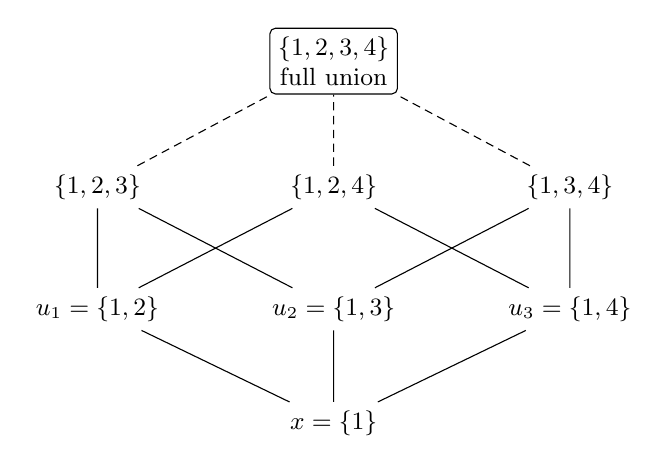
\begin{tikzpicture}[x=1cm,y=1cm,
  face/.style={fill=white,inner sep=3pt},
  every node/.style={font=\small}]
\node[face] (x) at (0,0) {$x=\{1\}$};
\node[face] (u1) at (-3,1.45) {$u_1=\{1,2\}$};
\node[face] (u2) at (0,1.45) {$u_2=\{1,3\}$};
\node[face] (u3) at (3,1.45) {$u_3=\{1,4\}$};
\node[face] (w12) at (-3,3) {$\{1,2,3\}$};
\node[face] (w13) at (0,3) {$\{1,2,4\}$};
\node[face] (w23) at (3,3) {$\{1,3,4\}$};
\node[face,draw,rounded corners=2pt,align=center] (all) at (0,4.6)
  {$\{1,2,3,4\}$\\full union};
\draw (x)--(u1) (x)--(u2) (x)--(u3);
\draw (u1)--(w12) (u1)--(w13);
\draw (u2)--(w12) (u2)--(w23);
\draw (u3)--(w13) (u3)--(w23);
\draw[densely dashed] (w12)--(all) (w13)--(all) (w23)--(all);
\end{tikzpicture}
\caption{The original Boolean faces containing $x$. Each pair among
$u_1,u_2,u_3$ has a proper union, but their total union is full.
All displayed subset relations survive the private insertions.
In the extension configuration of Proposition~\ref{ext:reduction},
solid edges correspond to restrictions of compatible homomorphisms
on actual nested domains. The dashed edges reach the full union,
for which a common extension is forbidden.}
\label{fig:boolean-faces}
\end{figure}


\section{From subgroup intervals to extensions}
\label{ext:section}

We now apply the decorated lattice of Proposition~\ref{lat:decorated-lattice}.
The reductions in this section use its tests in both orientations.  The
simple group attached to the top of the original group interval will be
denoted by $T$.  The simple group attached to an interval of extension
domains will later be denoted by $R$; these groups need not be isomorphic.

\begin{lemma}\label{ext:almost-simple}
Let $T$ be a finite nonabelian simple group and let
$\operatorname{Inn}(T)\le H\le\operatorname{Aut}(T)$.
Every nontrivial normal subgroup of $H$ contains $\operatorname{Inn}(T)$.
In particular, $H$ has trivial soluble radical and has characteristic
socle $\operatorname{Inn}(T)$.
\end{lemma}
\begin{proof}
An automorphism $\sigma$ centralizing every inner automorphism satisfies
$c_{\sigma(t)}=c_t$ for every $t\in T$.  Since $Z(T)=1$, this implies
$\sigma(t)=t$ for every $t$, so
$C_{\operatorname{Aut}(T)}(\operatorname{Inn}(T))=1$.
If $K\trianglelefteq H$, then
\[
 [K,\operatorname{Inn}(T)]\le K\cap\operatorname{Inn}(T).
\]
Simplicity makes the intersection either trivial or all of
$\operatorname{Inn}(T)$.  In the first case the centralizer calculation
gives $K=1$.  This proves the assertions.
\end{proof}

\begin{lemma}\label{ext:soluble-interval}
A nontrivial fenced interval cannot be an interval in a finite soluble
group.  Consequently, if
$\operatorname{Inn}(T)\le B\le H\le\operatorname{Aut}(T)$, the interval
$[B,H]$ is not nontrivially fenced.
\end{lemma}
\begin{proof}
Lemma~\ref{frm:labels} would give a nonabelian simple composition factor
of the soluble top group.  For the second assertion, quotient by
$\operatorname{Inn}(T)$, which is contained in the bottom $B$.
The resulting interval lies in the soluble group
$\operatorname{Out}(T)$, by Schreier's Theorem.
\end{proof}

\subsection{Minimality in both orientations}

Let $\mathcal L$ be the lattice in
Proposition~\ref{lat:decorated-lattice}.  Suppose that one of $\mathcal L$
and $\mathcal L^{\mathrm{op}}$ is a finite group interval.  Among all
representations of either orientation choose
\[
             [D,G]\cong\mathcal M,
       \qquad \mathcal M\in\{\mathcal L,\mathcal L^{\mathrm{op}}\},
\]
with $|G|$ minimal.  Minimizing over both orientations is the same
kind of reduction used in the subgroup-interval and signalizer setting
of \cite[Theorem~3 and Section~6]{Aschbacher2008}; see also the comparison in
\cite[Section~4]{PalfyTwisted}.  We give the needed complementary-socle
argument in full.  Quotienting by $\operatorname{core}_G(D)$ preserves
the interval; hence this core is trivial.  The global fence and
Lemma~\ref{frm:labels} give
\begin{equation}\label{ext:top-socle}
 S=\operatorname{soc}(G)=\prod_{i\in I}T_i\cong T^m,
 \qquad G=DS,
\end{equation}
where $T$ is nonabelian simple and $D$ acts transitively on the factor
set $I$.  Proposition~\ref{lat:decorated-lattice} applies to the chosen
orientation $\mathcal M$.

\begin{proposition}\label{ext:trivial-intersection}
In this minimal representation, $D\cap S=1$.
\end{proposition}
\begin{proof}
Put $E=D\cap S$.  For every $Y\in[D,G]$, the identity $G=DS$ gives
\[
                  Y=D(Y\cap S).
\]
Thus $Y\mapsto Y\cap S$ is an isomorphism from $[D,G]$ to the interval
of $D$-invariant subgroups between $E$ and $S$; its inverse is
$K\mapsto DK$.

First suppose that $E$ is subdirect in $S$.  By the subdirect-power
description in Lemma~\ref{frm:subdirect}, its simple factors are
full diagonal strips on a partition $\Pi$ of $I$.  Every subgroup
between $E$ and $S$ is subdirect.  Its strips split the blocks of $\Pi$,
and their diagonal identifications are forced by their containment of
$E$.  Therefore the preceding interval is anti-isomorphic to the
lattice of $D$-invariant equivalence relations refining $\Pi$.

Fix $i_0\in I$, let $A=D_{i_0}$, and let $B$ be the stabilizer in $D$
of the block of $\Pi$ containing $i_0$.  The block correspondence for a
transitive action identifies these equivalence relations with $[A,B]$:
the block containing $i_0$ associated with $U\in[A,B]$ is $U i_0$,
and all its other blocks are its $D$-translates.  Conversely, the
setwise stabilizer of the block containing $i_0$ recovers $U$.
It follows that $\mathcal M^{\mathrm{op}}\cong[A,B]$.  But
$|B|\le |D|<|G|$, contrary to the choice of $G$ over both orientations.

The coordinate projections of $E$ have equal order, since $D$ is
transitive on $I$.  If they are proper and nontrivial,
Proposition~\ref{frm:strict-product}, applied with the possibly unlabelled
lower endpoint $D$, and the global fence imply that $E$ is the product
of those projections.  Choose a proper original Boolean vertex $Y$
of the decorated lattice.  Its forward label equals the top label,
so $Y\cap S$ is subdirect by Proposition~\ref{frm:equal-transport}.
It is proper, because $Y<G$.

A product of nontrivial coordinate subgroups cannot lie in a proper
subdirect subgroup: the latter has a diagonal link between two
coordinates, whereas the former contains an element that is nontrivial
in one of those coordinates and trivial in the other.  This contradicts
$E\le Y\cap S$.  The only remaining possibility is that all coordinate
projections of $E$ are trivial, and then $E=1$.
\end{proof}

\subsection{The extension dictionary}

We give the parametrization with its group actions and order relations
explicit.  It is the induced-coordinate form of
\cite[Proposition~2.2 and Lemma~2.3]{PalfyTwisted}.

\begin{proposition}\label{ext:dictionary}
Let a finite group $D$ act on $S=\prod_{i\in I}T_i$, where all $T_i$
are isomorphic to a nonabelian simple group $T$, and suppose that its
action on $I$ is transitive.  Fix $i_0\in I$, set $A=D_{i_0}$, identify
$T_{i_0}$ with $T$, and let
$\alpha:A\to\operatorname{Aut}(T)$ be the induced action.

The $D$-invariant subdirect subgroups of $S$ are in bijection with pairs
$(U,\beta)$, where
\[
 A\le U\le D,\qquad
 \beta:U\longrightarrow\operatorname{Aut}(T),\qquad
 \beta|_A=\alpha.
\]
Write $S(U,\beta)$ for the corresponding subgroup.  Then
\begin{equation}\label{ext:dictionary-order}
 S(U,\beta)\le S(V,\gamma)
 \quad\Longleftrightarrow\quad
 V\le U\ \hbox{ and }\ \beta|_V=\gamma.
\end{equation}
In particular, the interval of $D$-invariant subgroups from
$S(U,\beta)$ to $S$ is anti-isomorphic to $[A,U]$, by restricting
$\beta$.
\end{proposition}
\begin{proof}
Use left conjugation for the given action and let $\pi_0:S\to T$ be
the chosen coordinate projection.  The map
\[
 s\longmapsto f_s,\qquad f_s(d)=\pi_0(d\cdot s),
\]
identifies $S$ with
\[
 \mathcal F_\alpha
 =\{f:D\to T:f(ad)=\alpha(a)(f(d))
                       \text{ for }a\in A,d\in D\}.
\]
Indeed, values on representatives of $A\backslash D$ are independent
coordinates of $S$.  Under this identification the action is
$(g\cdot f)(d)=f(dg)$.

An extension $\beta$ defines
\[
 \mathcal F_\beta
 =\{f:D\to T:f(ud)=\beta(u)(f(d))
                       \text{ for }u\in U,d\in D\}.
\]
This is a $D$-invariant subgroup of $\mathcal F_\alpha$, with independent
values on the cosets in $U\backslash D$.  Consequently
$\mathcal F_\beta\cong T^{[D:U]}$, and it projects onto every coordinate
of $\mathcal F_\alpha$.  Set $S(U,\beta)=\mathcal F_\beta$ in these
coordinates.

Conversely, let $K\le\mathcal F_\alpha$ be a $D$-invariant subdirect
subgroup.  Its diagonal-strip partition is invariant under the
transitive action on $A\backslash D$.  The block containing $A$ has
stabilizer $U$ for some $A\le U\le D$.  Projection at $1$ identifies
the diagonal factor on that block with $T$.  The induced action of $U$
on this factor gives a homomorphism
$\beta:U\to\operatorname{Aut}(T)$ extending $\alpha$.
For $f\in K$ and $u\in U$ one has $f(u)=\beta(u)(f(1))$.
Applying this identity to $d\cdot f$ gives
\[
                     f(ud)=\beta(u)(f(d)).
\]
Thus $K\le\mathcal F_\beta$.  Both groups have one freely varying
diagonal factor for each coset of $U$, so they are equal.

Containment of two subdirect groups reverses refinement of their strip
partitions.  Hence $S(U,\beta)\le S(V,\gamma)$ forces $V\le U$.
For $v\in V$, varying $f(1)$ over $T$ in the two defining equations
then gives $\beta(v)=\gamma(v)$.  The converse follows immediately
from those equations.  Finally, every subgroup containing a subdirect
subgroup is subdirect, so all members of the stated interval have
already been included.
\end{proof}

Apply Proposition~\ref{ext:dictionary} to
\eqref{ext:top-socle}.  By Proposition~\ref{ext:trivial-intersection},
the full interval $[D,G]$ is the lattice of $D$-invariant subgroups of
$S$, via $Y\mapsto Y\cap S$.  Whenever $Y\cap S$ is subdirect, write
$(U_Y,\beta_Y)$ for its extension.  In particular,
\begin{equation}\label{ext:actual-filter}
                  [Y,G]^{\mathrm{op}}\cong[A,U_Y].
\end{equation}
For nested filters these are compatible actual group intervals: the
larger domain's homomorphism restricts to the smaller domain's
homomorphism.  No representation of the entire dual lattice is asserted
by \eqref{ext:actual-filter}.

\subsection{The detector and the common image}

\begin{proposition}\label{ext:detector}
In the minimal representation fixed above, the induced factor-stabilizer
action $\alpha$ satisfies
$\alpha(A)\ge\operatorname{Inn}(T)$.
\end{proposition}
\begin{proof}
Let $X$ be the detector vertex of
Proposition~\ref{lat:decorated-lattice}.  Its forward type equals $T$, so
$E_X=X\cap S$ is subdirect in $S$.  The action of $D$ on the simple
factors of $E_X$ is transitive.  Its factor-stabilizer action is
$\beta_X:U_X\to\operatorname{Aut}(T)$ by the construction in
Proposition~\ref{ext:dictionary}.

Suppose that this action preserved a subgroup $1<P<T$.  Transporting
$P$ among the factors of $E_X$ would give a $D$-invariant product $Q$
of proper nontrivial coordinate subgroups of $E_X$.  Thus $DQ$ is
strictly between $D$ and $X$.  Choose a coatom $Y$ of $[D,X]$ containing
$DQ$.  The detector's coatom property gives a designated vertex
$d\le Y$ whose intersection $d\cap S$ is subdirect in the global
coordinates.  Hence $Y\cap S$ projects onto every simple factor of
$E_X$: projection onto such a factor can be identified with projection
onto any one global coordinate in its diagonal support.
Thus $Y\cap S$ is a proper subdirect subgroup of $E_X$ containing the
product $Q$, which is impossible by the diagonal-link argument in
Proposition~\ref{ext:trivial-intersection}.

The automorphism lemma recalled by P\'alfy
\cite[Lemma~2.11]{PalfyTwisted} states that a subgroup of
$\operatorname{Aut}(T)$ not containing $\operatorname{Inn}(T)$
preserves some proper nontrivial subgroup of $T$.
It follows that
\[
                 \beta_X(U_X)\ge\operatorname{Inn}(T).
\]

The reverse detector interval is the actual interval $[A,U_X]$ in
\eqref{ext:actual-filter}, and it is fenced.  Set $K=\ker\beta_X$.
Lemma~\ref{frm:normal-test} gives either $AK=U_X$ or $K\le A$.
The first possibility gives
$\beta_X(U_X)=\beta_X(A)=\alpha(A)$, as required.

In the second possibility $K\le C_X=\operatorname{core}_{U_X}(A)$,
and $[A,U_X]$ is represented as
\[
             [\alpha(A),\beta_X(U_X)].
\]
Write $H=\beta_X(U_X)$ and $B=\alpha(A)$.  If
$\operatorname{core}_H(B)$ is nontrivial, it contains
$\operatorname{Inn}(T)$ by Lemma~\ref{ext:almost-simple}.  Quotienting
by that core leaves a soluble top, contradicting
Lemma~\ref{ext:soluble-interval}.
Otherwise $C_X=K$, and $U_X/C_X\cong H$ has socle $T$ with multiplicity
one.  The reverse detector supplies a strictly smaller labelled domain
in $[A,U_X]$ whose simple type is equal to that of $U_X/C_X$.
The equality is supplied by the reverse tests in
Proposition~\ref{lat:decorated-lattice}, applied through
\eqref{ext:actual-filter}.  Proposition~\ref{frm:equal-transport} would make
its positive socle multiplicity strictly smaller than one.  This final
contradiction excludes $K\le A$.
\end{proof}

\begin{lemma}\label{ext:constant-image}
With $\alpha$ as in Proposition~\ref{ext:detector}, let $A<U\le D$ and
let $\beta:U\to\operatorname{Aut}(T)$ extend $\alpha$.
Suppose that $[A,U]$ is fenced.  Then
\[
                  U=A\ker\beta,
       \qquad \beta(U)=\alpha(A).
\]
\end{lemma}
\begin{proof}
The normal-subgroup test gives the asserted supplementation unless
$\ker\beta\le A$.  In the latter case $[A,U]$ is isomorphic to
$[\alpha(A),\beta(U)]$.  Proposition~\ref{ext:detector} puts the inner
group in its bottom, contrary to Lemma~\ref{ext:soluble-interval}.
Supplementation gives the equality of images.
\end{proof}

\begin{proposition}[The Boolean extension configuration]
\label{ext:reduction}
If either orientation of the decorated lattice has a finite-group
interval representation, there are finite groups $A\le D$, finite
nonabelian simple groups $T,R$, a homomorphism
$\alpha:A\to\operatorname{Aut}(T)$, and extensions
\[
 \beta_J:U_J\to\operatorname{Aut}(T)
       \qquad(\varnothing\ne J\subsetneq\{1,\ldots,4\})
\]
with the following properties.  Set $U_\varnothing=A$ and
$\beta_\varnothing=\alpha$.
\begin{enumerate}[label=\textup{(E\arabic*)}]
\item\label{ext:e1}
For nonempty proper $J$, $[A,U_J]$ is fenced.  If
$C_J=\operatorname{core}_{U_J}(A)$, the group $U_J/C_J$ has unique
minimal normal subgroup
\[
 N_J/C_J\cong R^{I_J},\qquad U_J=AN_J.
\]
\item\label{ext:e2}
If $J\subsetneq K\subsetneq\{1,\ldots,4\}$, then $U_J<U_K$ and
$\beta_K|_{U_J}=\beta_J$.  For nonempty $J$, the equal-type transport
of Proposition~\ref{frm:equal-transport} applies: in particular
\[
 \frac{U_J\cap N_K}{C_K}\ \cong\ \frac{N_J}{C_J},
 \qquad N_J=(U_J\cap N_K)C_J,
\]
and the canonical surjections $I_K\to I_J$ are $U_J$-equivariant and compose.
Whenever a nonempty family of proper subsets has proper union $K$, its domains
generate $U_K$.
\item\label{ext:e3}
All images $\beta_J(U_J)$ equal
$H=\alpha(A)\ge\operatorname{Inn}(T)$.
\item\label{ext:e4}
If a family of proper nonempty subsets has union $\{1,\ldots,4\}$,
its homomorphisms have no common extension to the subgroup of $D$
generated by their domains.
\end{enumerate}
\end{proposition}
\begin{proof}
Use the minimal representation already chosen.  Index the original
Boolean component in its reverse order by subsets $J$ of
$\{1,\ldots,4\}$.  Let $Y_J$ be the corresponding forward group, so
$Y_\varnothing=G$ and $Y_{\{1,\ldots,4\}}=D$.
Every proper nontrivial $Y_J$ has the top forward type and hence a
subdirect intersection with $S$.  Proposition~\ref{ext:dictionary}
provides $(U_J,\beta_J)$.

The reverse labels and tests in
Proposition~\ref{lat:decorated-lattice} apply in the actual filters
\eqref{ext:actual-filter}.  They give the fences and equal simple types
on comparable proper Boolean nodes.  All the nonempty proper nodes
therefore have one common simple type $R$: connect two atoms through
their proper two-atom join, and connect any other node to an atom below
it.  Lemma~\ref{frm:labels} and Proposition~\ref{frm:equal-transport} prove
\ref{ext:e1} and the transport assertions in \ref{ext:e2}.
The order relation and restrictions follow from
\eqref{ext:dictionary-order}.

For the assertion about a proper join, let $K$ be the union of a
nonempty family of index sets, and put
$V=\langle U_J:J\text{ in the family}\rangle$.
Then $A\le V\le U_K$, and $\beta_K|_V$ is an extension of all the
$\beta_J$.  Its subdirect group is contained in every $Y_J\cap S$
and contains $Y_K\cap S$.  Original Boolean meets are preserved in the
decorated lattice, so the intersection of those $Y_J$ is exactly
$Y_K$.  The subdirect groups are equal; the dictionary gives $V=U_K$.

Proposition~\ref{ext:detector} and Lemma~\ref{ext:constant-image} give
\ref{ext:e3}.  Finally, a common extension for a family with full union
would give a nontrivial subdirect subgroup of $S$ contained in all the
$Y_J\cap S$.  Their intersection is $D\cap S=1$, because their reverse
Boolean join is the top.  This proves \ref{ext:e4}.
\end{proof}

\section{Boolean gluing of extensions}
\label{glue:section}

We prove that the configuration in Proposition~\ref{ext:reduction}
cannot exist.  Throughout this section, $T$ is the target simple group
of the homomorphisms, whereas $R$ is the simple type of the domain
socles.  We retain the notation $A,D,H,U_J,\beta_J,C_J,N_J,I_J$ of
that proposition.  All extension domains lie in the finite group $D$.

The extensions will glue if their domain cores have images containing
$\operatorname{Inn}(T)$.  We first prove this criterion: a least normal
subgroup of $A$ with that image is normalized by every domain, and
conjugation on its simple quotient supplies the common extension.
We then force the criterion on the Boolean faces.  For an atom $x$,
the normal image $\alpha(C_x)$ is either trivial or contains the inner
group.  In the trivial case, compatible lifts from the three rank-two
faces through $x$ produce a different common extension, again forbidden
by \ref{ext:e4}.  Hence every atom core retains the inner group;
intersections pass this property to the larger proper faces.

\subsection{A criterion for extending over generated domains}

We begin with the elementary fact that makes least subgroups with a
prescribed perfect image available.

\begin{lemma}[Intersections retaining a perfect image]
\label{glue:perfect-intersections}
Let $f:M\to H_0$ be a homomorphism of finite groups, let $P\le H_0$
be perfect, and let $B_1,\ldots,B_s\trianglelefteq M$, with $s\ge1$, satisfy
$P\le f(B_i)$ for every $i$.  Then
\[
                  P\le f\left(\bigcap_{i=1}^s B_i\right).
\]
\end{lemma}
\begin{proof}
For two normal subgroups,
\[
 f(B_1\cap B_2)\ \supseteq\ f([B_1,B_2])
   =[f(B_1),f(B_2)]\ \supseteq\ [P,P]=P.
\]
Induction proves the assertion for the finite family.
\end{proof}

The following criterion applies to any finite family of extension
domains.  It will be used at the end with two rank-three Boolean faces
whose union is full.

\begin{lemma}[A common core and its conjugation extension]
\label{glue:common-core}
Let $A\le U_i\le D$ be a finite nonempty family of subgroups of a finite
group.  Let $T$ be nonabelian simple and suppose that homomorphisms
\[
 \alpha:A\to\operatorname{Aut}(T),\qquad
 \beta_i:U_i\to\operatorname{Aut}(T)
\]
satisfy
\[
 \beta_i|_A=\alpha,
 \qquad
 \alpha\bigl(\operatorname{core}_{U_i}(A)\bigr)
                         \ge\operatorname{Inn}(T).
\]
Put $K=\langle U_i:i\rangle$.  Then
$\alpha(\operatorname{core}_K(A))\ge\operatorname{Inn}(T)$, and there
is a unique homomorphism $\beta:K\to\operatorname{Aut}(T)$ extending
all the $\beta_i$.
\end{lemma}
\begin{proof}
Write $J=\operatorname{Inn}(T)$ and let
$\iota:T\to J$ be the isomorphism $t\mapsto c_t$.
Consider
\[
 Q=\bigcap\{B\trianglelefteq A:\alpha(B)\ge J\}.
\]
The family is nonempty.  Since $J$ is perfect,
Lemma~\ref{glue:perfect-intersections} shows that its finite
intersection still maps over $J$.  The subgroup $\alpha^{-1}(J)$
belongs to the family, so in fact
\begin{equation}\label{glue:least-perfect-image}
                         \alpha(Q)=J.
\end{equation}
Thus $Q$ is the least normal subgroup of $A$ with image containing $J$.

Fix $i$ and put $C_i=\operatorname{core}_{U_i}(A)$.  The hypothesis
gives $Q\le C_i$.  Make the analogous construction in $C_i$:
\[
 Q_i=\bigcap\{B\trianglelefteq C_i:\alpha(B)\ge J\}.
\]
The same intersection argument, using $C_i\cap\alpha^{-1}(J)$,
gives $\alpha(Q_i)=J$.
For $u\in U_i$ and $c\in C_i$,
\[
       \alpha(ucu^{-1})
          =\beta_i(u)\alpha(c)\beta_i(u)^{-1}.
\]
Since $C_i\trianglelefteq U_i$ and
$J\trianglelefteq\operatorname{Aut}(T)$, conjugation by $U_i$ permutes
the defining family for $Q_i$.  Thus $Q_i\trianglelefteq U_i$, and in
particular $Q_i\trianglelefteq A$.  Minimality of $Q$ gives $Q\le Q_i$.
Conversely, $Q\le C_i$, $Q\trianglelefteq C_i$, and
\eqref{glue:least-perfect-image} give $Q_i\le Q$.
Consequently $Q_i=Q$ for every $i$.

It follows that $Q\trianglelefteq K$ and
$Q\le\operatorname{core}_K(A)$, proving the common-core assertion.
Set $L=Q\cap\ker\alpha$.  Since
$L=Q\cap\ker\beta_i$ for every $i$, the subgroup $L$ is normalized by
each $U_i$ and therefore by $K$.
The map
\[
 \vartheta:Q/L\longrightarrow T,
        \qquad \vartheta(qL)=\iota^{-1}(\alpha(q))
\]
is an isomorphism.  Transporting the conjugation action of $K$ on
$Q/L$ through $\vartheta$ defines a homomorphism
$\beta:K\to\operatorname{Aut}(T)$.
For $u\in U_i$ and $q\in Q$,
\[
 \alpha(uqu^{-1})
 =\beta_i(u)\alpha(q)\beta_i(u)^{-1}
 =\iota\bigl(\beta_i(u)(\vartheta(qL))\bigr).
\]
As $\vartheta$ is onto, this proves $\beta|_{U_i}=\beta_i$.
These restrictions determine $\beta$ uniquely because the $U_i$
generate $K$.
\end{proof}

\subsection{An atom whose core is killed}

For $B\subseteq I_J$, let
\begin{equation}\label{glue:support-preimage}
 N_J(B)=q_J^{-1}\left(\prod_{i\in B}S_{J,i}\right),
 \qquad
 q_J:N_J\longrightarrow S_J=N_J/C_J,
\end{equation}
where $S_{J,i}$ are the simple direct factors of $S_J$.
Thus $N_J(\varnothing)=C_J$.  For comparable nonempty index sets
$J\subset K$, write $p_{KJ}:I_K\to I_J$ for the canonical factor map.

\begin{lemma}\label{glue:factorization}
If $x$ is an original Boolean atom and $\alpha(C_x)=1$, then
$\beta_x$ factors through the permutation action of $U_x$ on $I_x$.
\end{lemma}
\begin{proof}
By \ref{ext:e3}, $U_x=A\ker\beta_x$.  Since $A<U_x$ and $C_x\le A$,
the kernel is not contained in $C_x$.  The assumption makes
$\beta_x$ a homomorphism on $U_x/C_x$, so its nontrivial kernel there
contains the unique minimal normal subgroup $N_x/C_x$.
Consequently $\beta_x(N_x)=1$.

Let $P$ be the kernel of the action of $U_x$ on $I_x$.
Modulo $C_x$, the faithful conjugation action on $S_x$ embeds
$P/N_x$ into $\operatorname{Out}(R)^{I_x}$.  To justify faithfulness,
the centralizer of $S_x$ in $U_x/C_x$ is normal and disjoint from
$S_x$; uniqueness of the nonabelian minimal normal subgroup makes it
trivial.  Schreier's Theorem therefore makes $P/N_x$ soluble.
Its image under $\beta_x$ is a soluble normal subgroup of
$H=\alpha(A)$.  Lemma~\ref{ext:almost-simple} makes that image trivial,
so $P\le\ker\beta_x$, as claimed.
\end{proof}

Fix an atom $x$.  To rule out $\alpha(C_x)=1$, we shall show that this assumption
produces a subgroup $L$ normalized by $A$, generated by subgroups on
which the local extensions are trivial.  The remaining
condition for the formula $\theta(a\ell)=\alpha(a)$ to define an
extension on $AL$ is $A\cap L\le\ker\alpha$.  By Lemma~\ref{glue:factorization}, it is
enough to prove that every element of $A\cap L$ fixes the factor set
$I_x$.  The three proper faces through $x$ provide the local generators;
their proper pairwise joins will let us compare different factor labels.

Set
\[
 \mathcal U_x=\{x\cup\{a\}:a\in\{1,\ldots,4\}\setminus x\}.
\]
This family has three members.  Distinct $u,v\in\mathcal U_x$ have a
proper join $w=u\cup v$ of rank three.  For $j\in I_x$ and
$y\supseteq x$, write
\[
                   F_{y,j}=p_{yx}^{-1}(j),
       \qquad F_{x,j}=\{j\}.
\]
All factor maps in this notation are defined on proper nodes.
Figure~\ref{fig:boolean-faces} displays these three faces and their
proper pairwise joins.

A lift of the fibre $F_{u,j}$ must lie over the corresponding support
$F_{u\cup v,j}$ in each proper pair join $u\cup v$.  We therefore intersect its support
preimages in all those joins.  The perfect-image intersection lemma
ensures that these simultaneous requirements do not lose any factor
of the desired fibre.

\begin{lemma}[Compatible lifts of the fibres]
\label{glue:lifts}
For $u\in\mathcal U_x$ and $j\in I_x$, define
\begin{equation}\label{glue:Luj}
 L_{u,j}=N_u(F_{u,j})\cap
       \bigcap_{\substack{v\in\mathcal U_x\\v\ne u}}
       \bigl(U_u\cap N_{u\cup v}(F_{u\cup v,j})\bigr).
\end{equation}
These subgroups have the following properties.
\begin{enumerate}[label=\textup{(\roman*)}]
\item They are normal in $N_u$, and
$q_u(L_{u,j})=\prod_{i\in F_{u,j}}S_{u,i}$.
\item Conjugation by $U_x$ permutes the choices according to its action
on $I_x$.  In particular, $C_x$ normalizes every $L_{u,j}$.
\item $U_u=\langle A,L_{u,j}:j\in I_x\rangle$.
\item For $j\ne k$, one has
\[
 [L_{u,j},L_{v,k}]\le
 \begin{cases}
 C_{u\cup v},&u\ne v,\\
 C_u,&u=v.
 \end{cases}
\]
Both right-hand sides are contained in $C_x$.
\item If $\alpha(C_x)=1$, then $\beta_u(L_{u,j})=1$ for all $u,j$.
\end{enumerate}
\end{lemma}
\begin{proof}
Fix a proper pair join $w=u\cup v$.  Equal-type transport gives
\begin{equation}\label{glue:Nu-transport}
                  N_u=(U_u\cap N_w)C_u.
\end{equation}
The first factor on the right acts by inner automorphisms on
$N_w/C_w$, hence preserves every coordinate subproduct there.
The second factor satisfies $C_u\le C_x\le U_x$.  Since $C_x$ acts
trivially on $I_x$, equivariance of $p_{wx}$ says that $C_u$ fixes the
set $F_{w,j}$.  It too normalizes $N_w(F_{w,j})$.
Thus $U_u\cap N_w(F_{w,j})$ is normal in $N_u$ and lies in $N_u$.

In $N_w/C_w$, the subdirect group $(U_u\cap N_w)/C_w$ has its diagonal
strips indexed by $I_u$.  Their supports are the fibres of $p_{wu}$.
Because $p_{wx}=p_{ux}p_{wu}$, intersecting with the $F_{w,j}$-support
product selects exactly the strips indexed by $F_{u,j}$.
The isomorphism from this subdirect group to $N_u/C_u$ therefore shows
that $U_u\cap N_w(F_{w,j})$ maps onto
$\prod_{i\in F_{u,j}}S_{u,i}$ under $q_u$.
The first group in \eqref{glue:Luj} is normal in $N_u$ and has the same
image.  This image is perfect.  Lemma~\ref{glue:perfect-intersections}
proves (i).

Every domain occurring in \eqref{glue:Luj} contains $U_x$, and all the
factor maps are $U_x$-equivariant.  Its conjugation therefore permutes
the whole definition with $j$, proving (ii).  The images in (i)
generate $N_u/C_u$, and $C_u\le A$; since $U_u=AN_u$, this proves (iii).

For $u\ne v$, the two lifts in (iv) lie in disjoint coordinate support
products of $N_{u\cup v}/C_{u\cup v}$.  They commute in that quotient.
For $u=v$ the identical argument takes place in $N_u/C_u$.
Core inclusion along $U_x\le U_u\le U_{u\cup v}$ gives the asserted
containment in $C_x$.

Finally suppose that $\alpha(C_x)=1$.  Then $\beta_u(C_u)=1$.
The kernel of $\beta_u$ supplements $A$ and is not contained in $C_u$,
so it contains $N_u$ by the unique-minimal-normal-subgroup argument in
Lemma~\ref{glue:factorization}.  This proves (v).
\end{proof}

We next construct subgroups $B_k$ which distinguish the labels
$k\in I_x$ and are normalized by every lift with a different label.
Different labels commute only modulo $C_x$, and $C_x$ need not be
normal in the group generated by all the lifts.  The following finite
core argument keeps a full simple image without requiring that
normality.

\begin{lemma}[Taking cores without losing a simple image]
\label{glue:retained-core}
Let $R_0\le D$, let $C\trianglelefteq R_0$, and suppose that
$R_0/C$ is nonabelian simple.  Let $L_1,\ldots,L_s\le D$ be normalized
by $R_0$.  Suppose that, for every $t$, there is a subgroup
$D_t\trianglelefteq R_0$ such that
\[
 D_tC=R_0,\qquad D_t^{L_t}=D_t,
 \qquad [D_t,L_t]\le D_t\cap C.
\]
Then, for $W=\langle R_0,L_1,\ldots,L_s\rangle$, the subgroup
$\operatorname{core}_W(R_0)$ maps onto $R_0/C$.
No normalization of $C$ by $L_t$ is assumed.
\end{lemma}
\begin{proof}
Let $\pi:R_0\to R_0/C$ be the quotient map.  Start with $B=R_0$.
At every stage $B$ will be normal in $R_0$ and satisfy
$\pi(B)=R_0/C$.  For a fixed $t$, replace $B$ by
\begin{equation}\label{glue:core-operation}
       F_t(B)=\bigcap_{\ell\in L_t}(B\cap D_t)^\ell,
       \qquad K^\ell=\ell^{-1}K\ell.
\end{equation}
The subgroup $B\cap D_t$ still maps onto $R_0/C$ by
Lemma~\ref{glue:perfect-intersections}.  Put $K=B\cap D_t$.  The subgroup $K$ is normal in $D_t$, because
$B\trianglelefteq R_0$ and $D_t\leq R_0$.  Since $L_t$ normalizes
$D_t$, every conjugate $K^\ell$ lies in $D_t$ and is normal in $D_t$.
For $d\in D_t$ and $\ell\in L_t$, the assumption
$[D_t,L_t]\leq D_t\cap C$ gives $\pi(d^\ell)=\pi(d)$.
Consequently $\pi(K^\ell)=\pi(K)=R_0/C$ for every $\ell$.
This applies the quotient map only to elements of $D_t\leq R_0$;
it does not require $C$ to be normalized by $L_t$.  Applying
Lemma~\ref{glue:perfect-intersections} inside $D_t$ shows that $F_t(B)$
has full image.

The new subgroup is normal in $R_0$.  Indeed, $R_0$ normalizes $B$, $D_t$, and $L_t$.  For $r\in R_0$
one therefore has $(K^\ell)^r=(K^r)^{\ell^r}=K^{\ell^r}$, and
$\ell^r\in L_t$.  Thus $R_0$ permutes precisely the conjugates
intersected in \eqref{glue:core-operation}.  The operation is descending, since the
identity conjugate occurs.  Apply $F_1,\ldots,F_s$ in repeated rounds.
Finiteness forces stabilization, and at a stable round every
intermediate inclusion is equality.  The resulting subgroup $B_*$
is therefore normalized by each $L_t$ as well as by $R_0$.  Thus
$B_*\trianglelefteq W$ and $B_*\le R_0$, while
$\pi(B_*)=R_0/C$.  Since
$B_*\le\operatorname{core}_W(R_0)$, the asserted core also has full
image.
\end{proof}

\begin{lemma}[Subgroups detecting the factor labels]
\label{glue:detectors}
Put $L_j=\langle L_{u,j}:u\in\mathcal U_x\rangle$ and
$R_k=N_x(\{k\})$.  There are subgroups $B_k\le R_k$, for $k\in I_x$,
such that
\begin{enumerate}[label=\textup{(\roman*)}]
\item $q_x(B_k)=S_{x,k}$;
\item every $L_j$ with $j\ne k$ normalizes $B_k$;
\item $C_x$ normalizes every $B_k$, and $A$ permutes the $B_k$ in the
same way as it permutes $I_x$.
\end{enumerate}
In particular, the subgroups $B_k$ are pairwise distinct.
\end{lemma}
\begin{proof}
For $u\in\mathcal U_x$ set
\[
                     D_{u,k}=U_x\cap N_u(F_{u,k}).
\]
The transported subdirect group $(U_x\cap N_u)/C_u$ maps isomorphically
onto $N_x/C_x$.  Selecting its strips over $k$ shows that
\begin{equation}\label{glue:Duk}
 D_{u,k}\le R_k,\quad D_{u,k}C_x=R_k,
 \quad D_{u,k}\cap C_x=C_u.
\end{equation}
It is normal in $R_k$: all elements of $R_k\le N_x$ fix the factor
labels $I_x$, and the support-preimage construction is equivariant.

For $j\ne k$, both $D_{u,k}$ and $L_{u,j}$ lie in $N_u$ and have
disjoint supports modulo $C_u$.  Thus
\[
                    [D_{u,k},L_{u,j}]\le C_u.
\]
Since $C_u\le D_{u,k}$, this also proves that $L_{u,j}$ normalizes
$D_{u,k}$.  Moreover $R_k$ normalizes $L_{u,j}$ by
Lemma~\ref{glue:lifts}(ii), since $R_k$ fixes every label of $I_x$.
We can therefore apply Lemma~\ref{glue:retained-core} to $R_k$, its
normal subgroup $C_x$, and all the lifts $L_{u,j}$ with $j\ne k$, using
the subgroup $D_{u,k}$ for the lift labelled by $(u,j)$.

Define canonically
\[
 W_k=\langle R_k,L_j:j\ne k\rangle,
 \qquad B_k=\operatorname{core}_{W_k}(R_k).
\]
That lemma proves (i); the definition proves (ii).
Since $C_x\le R_k\le W_k$, it normalizes $B_k$.
Conjugation by $A$ permutes the pairs $(W_k,R_k)$ and hence their
cores, proving (iii).  Their images in $N_x/C_x$ are the distinct
nontrivial coordinate factors, so the $B_k$ are distinct.
\end{proof}

To use the subgroups $B_k$, we must collect all letters with one
chosen label at the end of a word in the lifts.  The errors lie in
$C_x$, which normalizes each individual lift.  The following word
calculation records exactly the form needed.

\begin{lemma}[Collection with labelled factors]
\label{glue:collection}
Let $C\le D$ normalize subgroups $P_\lambda\le D$ indexed by a finite
set.  Assign each index a label $c(\lambda)\in I$.  Suppose that
\[
 [P_\lambda,P_\mu]\le C
                \quad\text{whenever }c(\lambda)\ne c(\mu).
\]
Put $L_j=\langle P_\lambda:c(\lambda)=j\rangle$ and
$L=\langle L_j:j\in I\rangle$.  For every $k\in I$, every element
$g\in L$ can be written
\[
        g=pqc,\qquad
        p\in\langle L_j:j\ne k\rangle,\quad q\in L_k,\quad c\in C.
\]
\end{lemma}
\begin{proof}
Write $g$ as a word whose letters belong to the individual
$P_\lambda$; inverses are allowed because these are subgroups.
Interchange adjacent letters with different labels to move the
$k$-labelled letters to the end.  Each interchange introduces a
commutator in $C$.  Move that error to the right through the remaining
word, using
\[
                    c\ell=(c\ell c^{-1})c.
\]
The conjugated letter remains in its original $P_\lambda$, so its
label does not change.  Each interchange reduces the number of pairs
consisting of a $k$-letter preceding a non-$k$-letter.  The process
terminates with the asserted expression.  This is a word calculation;
it does not form a quotient by $C$ or require $C\trianglelefteq L$.
\end{proof}

\begin{proposition}\label{glue:atom-cores}
For every original Boolean atom $x$,
$\alpha(C_x)\ge\operatorname{Inn}(T)$.
\end{proposition}
\begin{proof}
The subgroup $\alpha(C_x)$ is normal in
$\beta_x(U_x)=H$.  Lemma~\ref{ext:almost-simple} reduces the assertion
to excluding $\alpha(C_x)=1$.  Assume that equality and use the lifts
and detecting subgroups just constructed.  Put
\[
                         L=\langle L_j:j\in I_x\rangle.
\]
The group $A$ normalizes $L$.

Let $a\in A\cap L$.  We show that $a$ fixes every member of $I_x$.
For subgroup conjugation use the right-action notation
$K^g=g^{-1}Kg$.  If $a$ sent $k$ to $h\ne k$, equivariance would give
$B_k^a=B_h$.  Lemmas~\ref{glue:lifts} and~\ref{glue:collection}, with
$C=C_x$ and the individual $L_{u,j}$ as labelled subgroups, give
\[
        a=pqc,\qquad
        p\in\langle L_j:j\ne k\rangle,\quad q\in L_k,\quad c\in C_x.
\]
The element $p$ normalizes $B_k$, $q$ normalizes $B_h$, and $c$
normalizes both.  It follows successively that
\[
                 B_k^{qc}=B_h,
       \qquad B_k^q=B_h,
       \qquad B_k=B_h,
\]
contradicting Lemma~\ref{glue:detectors}.  Thus $a$ fixes the factor
set.  Lemma~\ref{glue:factorization} now gives $\alpha(a)=1$.

Consequently $A\cap L\le\ker\alpha$.  Because $A$ normalizes $L$,
the formula
\[
              \theta:AL\longrightarrow\operatorname{Aut}(T),
                       \qquad \theta(a\ell)=\alpha(a)
\]
defines a homomorphism.  It is well defined by the intersection
inclusion; multiplication is respected since $L\trianglelefteq AL$.
For each $u\in\mathcal U_x$, Lemma~\ref{glue:lifts}(iii),(v) says that
$U_u$ is generated by $A$ and lifts killed by both $\theta$ and
$\beta_u$.  Hence $\theta|_{U_u}=\beta_u$.

The three sets $u\in\mathcal U_x$ have full union
$\{1,\ldots,4\}$.  Their generated domain is $AL$, so this common
extension contradicts \ref{ext:e4}.  The assumption
$\alpha(C_x)=1$ is impossible.
\end{proof}

\subsection{Compatible joins and the contradiction}

\begin{lemma}[Cores under a compatible join]
\label{glue:core-joins}
For every nonempty proper original Boolean node $z$,
\[
             C_z=\bigcap_{x\subseteq z,\,|x|=1}C_x.
\]
Consequently $\alpha(C_z)\ge\operatorname{Inn}(T)$.
\end{lemma}
\begin{proof}
The assertion is immediate for an atom, so suppose that $|z|\ge2$.
Every $C_x$ in the intersection contains $C_z$.  Pass to $U_z/C_z$
and use bars for the images of $A,U_x,C_x$.  Put
\[
 N=N_z/C_z,\qquad E_x=(U_x\cap N_z)/C_z.
\]
The transport isomorphism in \ref{ext:e2} gives
$E_x\cap\overline C_x=1$.  Both are normal in $\overline U_x$, so
$[E_x,\overline C_x]=1$.

Since $U_z=AN_z$ and $A\le U_x$, one has
$\overline U_x=\overline A E_x$.
Let $M=\langle E_x:x\subseteq z,\ |x|=1\rangle$.
Each $E_x$ is normalized by $\overline A$.  The compatible-join
generation in \ref{ext:e2} therefore gives
\[
                       \overline U_z=\overline A M,
\]
so $M\trianglelefteq\overline U_z$.  It is a nontrivial subgroup of
the minimal normal subgroup $N$, and hence $M=N$.
Thus $\bigcap_x\overline C_x$ centralizes $N$.
The centralizer is normal in $\overline U_z$ and intersects $N$ in
$Z(N)=1$.  If it were nontrivial it would contain the unique minimal
normal subgroup $N$, a contradiction.  The intersection is therefore
trivial, which proves the equality of cores.

Each $C_x$ is normal in $A$ and maps over $\operatorname{Inn}(T)$ by
Proposition~\ref{glue:atom-cores}.  Apply
Lemma~\ref{glue:perfect-intersections} with
$P=\operatorname{Inn}(T)$ to obtain the image assertion.
\end{proof}

\begin{theorem}\label{glue:contradiction}
The Boolean extension configuration of
Proposition~\ref{ext:reduction} does not exist.
\end{theorem}
\begin{proof}
Take the two proper Boolean nodes
\[
              z=\{1,2,3\},\qquad w=\{2,3,4\}.
\]
Lemma~\ref{glue:core-joins} gives
$\alpha(C_z),\alpha(C_w)\ge\operatorname{Inn}(T)$.
Lemma~\ref{glue:common-core} therefore extends $\beta_z$ and $\beta_w$
to $\langle U_z,U_w\rangle$.  Since $z\cup w=\{1,\ldots,4\}$, this
contradicts \ref{ext:e4}.
\end{proof}

\begin{proof}[Proof of Theorem~\ref{main:group}]
Choose the finite decorated lattice of
Proposition~\ref{lat:decorated-lattice}.  If either it or its dual had a
finite-group interval representation, Proposition~\ref{ext:reduction}
would produce the configuration excluded by
Theorem~\ref{glue:contradiction}.  Hence this lattice has no such
representation, proving Theorem~\ref{main:group}.
\end{proof}

Theorem~\ref{main:congruences} now follows from
Theorem~\ref{main:group} and the global P\'alfy--Pudl\'ak equivalence
\cite[Theorem~2]{PalfyPudlak1980}.


\bibliographystyle{plain}
\bibliography{references}
\end{document}

